% Drones, control y visión para principiantes: la simulación del Tarot 650
% que busca incendios. Compila con pdfLaTeX (por omisión en Overleaf), XeLaTeX o LuaLaTeX.
\documentclass[11pt,letterpaper,oneside,openany]{book}

\usepackage{iftex}
\ifPDFTeX
  \usepackage[utf8]{inputenc}
  \usepackage[T1]{fontenc}
  \usepackage{lmodern}
\else
  \usepackage{fontspec}
\fi
\usepackage[spanish,es-noshorthands,es-tabla]{babel}
\usepackage[margin=2.4cm]{geometry}
\usepackage{amsmath,amssymb}
\usepackage{graphicx}
\usepackage{booktabs,tabularx,array,longtable}
\usepackage{enumitem}
\usepackage[dvipsnames]{xcolor}
\usepackage[most]{tcolorbox}
\usepackage{listings}
\usepackage{tikz}
\usetikzlibrary{arrows.meta,positioning,shapes.geometric,shapes.misc,fit,calc,decorations.pathmorphing}
\usepackage{caption}
\usepackage{float}
\usepackage{xurl}
\usepackage[colorlinks=true,linkcolor=NavyBlue,urlcolor=NavyBlue,citecolor=NavyBlue]{hyperref}

\graphicspath{{figuras/}}
\setlist{itemsep=2pt,topsep=4pt}
\setlength{\parindent}{0pt}
\setlength{\parskip}{6pt}
\setlength{\emergencystretch}{3em}
\captionsetup{font=small,labelfont=bf}
\urlstyle{tt}

% Rutas, archivos, nodos y tópicos en monoespaciado (con _ y / sin escapar).
\newcommand{\cod}[1]{\expandafter\nolinkurl\expandafter{\detokenize{#1}}}
\newcommand{\sgn}{\operatorname{sgn}}
\newcommand{\Sgn}{\operatorname{Sgn}}

\lstset{basicstyle=\ttfamily\footnotesize,columns=fullflexible,keepspaces=true,breaklines=true,
        frame=single,rulecolor=\color{black!25},backgroundcolor=\color{black!3},
        xleftmargin=4pt,xrightmargin=4pt,aboveskip=6pt,belowskip=6pt,
        showstringspaces=false,upquote=true,
        literate={á}{{\'a}}1 {é}{{\'e}}1 {í}{{\'i}}1 {ó}{{\'o}}1 {ú}{{\'u}}1
                 {Á}{{\'A}}1 {É}{{\'E}}1 {Í}{{\'I}}1 {Ó}{{\'O}}1 {Ú}{{\'U}}1
                 {ñ}{{\~n}}1 {Ñ}{{\~N}}1 {ü}{{\"u}}1 {¿}{{?`}}1 {¡}{{!`}}1
                 {°}{{$^\circ$}}1 {²}{{$^2$}}1 {·}{{$\cdot$}}1 {→}{{$\rightarrow$}}1
                 {×}{{$\times$}}1 {±}{{$\pm$}}1 {—}{{---}}1 {–}{{--}}1}
\lstdefinestyle{bash}{language=bash,morekeywords={ros2,colcon,source,sudo,git,gz,python3}}
\lstdefinestyle{py}{language=Python,keywordstyle=\color{NavyBlue}\bfseries,commentstyle=\color{black!55}\itshape,
                    stringstyle=\color{BrickRed}}
\lstdefinestyle{xml}{language=XML,keywordstyle=\color{NavyBlue},stringstyle=\color{BrickRed}}

% Recuadros del libro.
\tcbset{enhanced,breakable,boxrule=0.6pt,arc=2pt,left=6pt,right=6pt,top=4pt,bottom=4pt,fonttitle=\bfseries}
\newtcolorbox{nota}{colback=NavyBlue!4,colframe=NavyBlue!70!black,title=Nota}
\newtcolorbox{aviso}{colback=BrickRed!5,colframe=BrickRed!70!black,title=Cuidado}
\newtcolorbox{leccion}{colback=ForestGreen!5,colframe=ForestGreen!70!black,title=Problema encontrado y cómo se resolvió}
\newtcolorbox{recuerda}{colback=Goldenrod!10,colframe=Goldenrod!80!black,title=Recuerda}
\newtcolorbox{consejo}{colback=Cyan!5,colframe=Cyan!60!black,title=Consejo}
\newtcolorbox{tecnico}{colback=black!3,colframe=black!45,title=Para curiosos (te lo puedes saltar)}
\newtcolorbox{ejemplo}[1][]{colback=Orchid!5,colframe=Orchid!70!black,title=Ejemplo de la vida diaria#1}
\newtcolorbox{ejercicio}{colback=Peach!8,colframe=Peach!80!black,title=Pruébalo tú}
\newtcolorbox{enpocas}{colback=ForestGreen!4,colframe=ForestGreen!50!black,title=En este capítulo}

\title{\textbf{Drones, control y visión}\\[4pt]
\textbf{para principiantes}\\[10pt]
\Large Cómo se construyó la simulación del Tarot Ironman 650\\ que busca incendios forestales por sí solo\\[8pt]
\large ROS 2 Jazzy · Gazebo Harmonic · ArduPilot SITL · YOLO26}
\author{Dr.\ Jairo Olguín Roque\\
FES Acatlán, UNAM}
\date{Octubre de 2026}

\begin{document}
\frontmatter
\maketitle
\tableofcontents
\chapter{Cómo usar este libro}

\section*{¿Para quién es?}

Para cualquier persona que quiera entender, desde cero, cómo funciona un dron que vuela solo:
estudiantes de licenciatura, ingenieros de otras áreas o curiosos. No
necesitas saber de drones, de control automático ni de inteligencia artificial. Sí ayuda saber
usar una computadora con Linux y recordar algo de física y matemáticas de bachillerato; cuando
haga falta algo más, lo explicamos en el momento.

El libro cuenta una historia real: cómo se construyó, en tres días de octubre de 2026, una
simulación para el monitoreo de incendios forestales. En ella un dron Tarot Ironman 650
despega, recorre un bosque de 420 por 420 metros, encuentra un incendio con su cámara, avisa
sus coordenadas GPS y se queda vigilándolo. Cada pieza de esa historia es una excusa para explicar
un concepto.

\section*{Cómo está organizado}

\begin{description}
  \item[Parte I. Lo básico.] Qué es un dron y cómo vuela, la física mínima que hace falta, qué es
        una simulación y qué es ROS~2, el ``sistema nervioso'' que conecta todas las piezas.
  \item[Parte II. El control.] Cómo se consigue que el dron vaya exactamente a donde queremos aunque
        sople el viento: control PID, modos deslizantes, super-twisting y el tema central del
        proyecto, la discretización implícita.
  \item[Parte III. Visión.] Qué es una imagen para una computadora, cómo funciona una cámara y cómo
        una red neuronal (YOLO) aprende a reconocer fuego y humo.
  \item[Parte IV. Construir la simulación.] La instalación y cómo se metieron en Gazebo el dron, sus
        motores, el bosque, las montañas, los animales y el incendio.
  \item[Parte V. Autonomía.] Cómo el dron decide qué hacer: recorrer el bosque, evitar árboles y
        montañas, estimar dónde está el fuego, confirmarlo y avisar. También cómo volar con un
        piloto automático real (ArduPilot).
  \item[Parte VI. Manos a la obra.] Un tutorial para hacer tu primer vuelo, la lista de órdenes y
        cómo se verificó que todo funciona.
\end{description}

Al final hay un \textbf{glosario} con todas las palabras raras.

Si solo quieres usar la simulación, puedes ir directo al capítulo~\ref{cap:primer-vuelo}
(``Tu primer vuelo''). Si quieres entenderla, léelo en orden: cada parte se apoya en la anterior.

\section*{Los recuadros}

\begin{recuerda}
Lo más importante del tema, en pocas palabras. Si solo lees esto, ya te llevas la idea.
\end{recuerda}

\begin{consejo}
Trucos prácticos que ahorran tiempo o problemas.
\end{consejo}

\begin{ejemplo}
Una comparación con algo cotidiano para entender un concepto abstracto.
\end{ejemplo}

\begin{tecnico}
Detalles matemáticos o de programación. Si es tu primera lectura, sáltalos sin culpa.
\end{tecnico}

\begin{aviso}
Errores que es fácil cometer y que pueden romper algo o hacerte perder horas.
\end{aviso}

\begin{leccion}
Problemas reales que aparecieron durante el desarrollo y cómo se resolvieron. Son de lo más
valioso del libro: así se trabaja de verdad.
\end{leccion}

\begin{ejercicio}
Algo que puedes hacer en la simulación para comprobar lo que acabas de leer.
\end{ejercicio}

\section*{Convenciones de escritura}

\begin{itemize}
  \item Las órdenes que se escriben en la terminal aparecen en recuadros grises:
\begin{lstlisting}[style=bash]
ros2 launch cuadrirotor_sim simulacion.launch.py
\end{lstlisting}
  \item Los nombres de archivos, programas y tópicos van en letra de máquina: \cod{busqueda_incendio}.
  \item \cod{~} significa tu carpeta personal (\cod{/home/tu_usuario}).
  \item Las distancias están en metros, los ángulos en radianes o grados (se indica) y el tiempo
        en segundos.
\end{itemize}


\mainmatter
\part{Antes de despegar: lo básico}
\chapter{El proyecto de un vistazo}

Este libro documenta, paso a paso, cómo se construyó la simulación de monitoreo de incendios:
desde la instalación del software hasta la misión autónoma en la que un cuadrirrotor
Tarot Ironman 650 recorre un bosque, encuentra un incendio con una cámara y una red neuronal,
envía sus coordenadas GPS y lo orbita. Todo el desarrollo se hizo entre el 21 y el 23 de
octubre de 2026 en el espacio de trabajo \cod{~/ros2_ws}.

\section{Qué hace la simulación}

\begin{itemize}
  \item \textbf{Planta.} Gazebo Harmonic simula la física del dron: cuerpo rígido, cuatro
        motores de primer orden con empuje $f_i = k_f\omega_i^2$, una cámara, una IMU y un
        LiDAR 3D. Hay dos vehículos: un cuadrirrotor genérico en ``+'' y el Tarot 650 en ``X'',
        cuya geometría viene de su CAD.
  \item \textbf{Control.} Tres alternativas intercambiables: un PD en cascada (línea base),
        el super-twisting adaptativo (STA) con tres discretizaciones (explícita,
        semi-implícita e implícita) y el piloto automático ArduCopter 4.7.2 en SITL.
  \item \textbf{Mundos.} Tres escenarios: \cod{incendio} (plano), \cod{bosque} (85 árboles) y
        \cod{bosque_grande}: un valle de $420\times420$~m rodeado de montañas, con 1700 árboles,
        140 rocas, 21 animales, cielo y un incendio con humo.
  \item \textbf{Percepción.} YOLO26n ajustado con 6000 imágenes del simulador detecta
        \emph{fuego} y \emph{humo} en la cámara del dron.
  \item \textbf{Autonomía.} El nodo \cod{busqueda_incendio} despega, barre el bosque en
        serpentina siguiendo el relieve, evita obstáculos con el LiDAR, estima la posición del
        foco, lo confirma con las llamas, avisa con las coordenadas GPS y lo orbita.
\end{itemize}

\section{Arquitectura}

La figura~\ref{fig:arquitectura} muestra los nodos y los tópicos principales. La cadena completa es
\emph{imagen $\rightarrow$ detección $\rightarrow$ estimación $\rightarrow$
referencia $\rightarrow$ control}. El planificador nunca usa la posición verdadera del foco:
solo lo que reporta el detector.

\begin{figure}[H]
\centering
\begin{tikzpicture}[
  nodo/.style={draw,rounded corners,fill=#1,minimum width=3.1cm,minimum height=1cm,align=center,font=\small},
  nodo/.default=white,
  flecha/.style={-{Stealth[length=2.5mm]},thick},
  et/.style={font=\scriptsize\ttfamily,fill=white,inner sep=1pt}]
  \node[nodo=orange!15,minimum width=4.2cm,minimum height=2.2cm] (gz) at (0,0)
       {\textbf{Gazebo Harmonic}\\ física, motores, cámara,\\ IMU, LiDAR, mundo};
  \node[nodo=black!5] (puente) at (0,-2.4) {\cod{ros_gz_bridge}\\(\cod{puente.yaml})};
  \node[nodo=blue!10] (yolo) at (-5,-4.6) {\cod{detector_yolo}\\YOLO26n (GPU)};
  \node[nodo=green!12,minimum width=4cm] (bus) at (0,-6.6) {\cod{busqueda_incendio}\\planificador autónomo};
  \node[nodo=red!10] (ctl) at (5,-4.6) {\cod{controlador_sta}\\ o \cod{controlador_pd}};
  \node[nodo=red!10] (ap) at (5,-8.6) {\cod{mision_ardupilot}\\+ ArduCopter SITL};
  \node[nodo=black!5] (fauna) at (-6.2,0) {\cod{fauna}\\(gz-transport)};
  \node[nodo=black!5] (viento) at (6.2,0) {\cod{viento}};
  \node[nodo=yellow!15] (alerta) at (-4.5,-8.6) {aviso GPS\\\cod{/cuadrirotor/incendio/*}};

  \draw[flecha] (gz) -- (puente);
  \draw[flecha] (puente) -| node[et,pos=0.75]{camara} (yolo);
  \draw[flecha] (yolo) |- node[et,pos=0.3]{detecciones} (bus);
  \draw[flecha] (puente) -- node[et]{odometria, lidar/points} (bus);
  \draw[flecha] (bus) -| node[et,pos=0.3]{consigna} (ctl);
  \draw[flecha] (bus) -| node[et,pos=0.3]{consigna} (ap);
  \draw[flecha] (ctl) |- node[et,pos=0.75]{motores} (puente);
  \draw[flecha] (ap.east) -- ++(2.6,0) |- node[et,pos=0.25,rotate=90]{MAVLink / JSON} ([yshift=-7mm]gz.east);
  \draw[flecha] (fauna) -- node[et,above=1pt]{set\_pose\_vector} (gz);
  \draw[flecha] ([yshift=3mm]viento.west) -- node[et,above=1pt]{viento} ([yshift=3mm]gz.east);
  \draw[flecha] (bus.south) |- (alerta.east);
\end{tikzpicture}
\caption{Nodos y tópicos de la misión de búsqueda. Con \cod{controlador:=sta} o \cod{pd} la
consigna la sigue el controlador de ROS~2; con \cod{controlador:=ardupilot}, la reenvía
\cod{mision_ardupilot} a ArduCopter por MAVLink.}
\label{fig:arquitectura}
\end{figure}

\section{Convenciones}

\begin{itemize}
  \item \textbf{Marco del mundo:} ENU (\emph{x} al este, \emph{y} al norte, \emph{z} arriba), en
        metros. ArduPilot usa NED: $N = y$, $E = x$, $D = -z$ y la guiñada NED es
        $\pi/2 - \psi$.
  \item \textbf{Marco del cuerpo:} \emph{x} al frente, \emph{y} a la izquierda, \emph{z} arriba.
  \item El modelo del dron se llama siempre \cod{cuadrirotor} dentro de Gazebo, sin importar
        el vehículo; así los tópicos no cambian.
  \item Rutas: el paquete principal está en \cod{~/ros2_ws/src/cuadrirotor_sim}; salvo que se
        diga otra cosa, las rutas relativas son respecto a él.
\end{itemize}

\section{Equipo usado}

Ubuntu 24.04 (Noble), ROS~2 Jazzy, Gazebo Harmonic (gz-sim 8), ArduCopter 4.7.2 y una GPU
NVIDIA RTX 5060 Ti (YOLO corre en la GPU y Gazebo renderiza con EGL de NVIDIA). Con este equipo
el mundo grande corre a tiempo real (factor $\approx 1.0$; $\approx 0.8$ con el LiDAR).

\chapter{¿Qué es un dron y cómo vuela?}

\begin{enpocas}
Las partes de un cuadrirrotor, por qué vuela, cómo sube, avanza y gira con solo cambiar la velocidad
de sus cuatro motores, y cómo es el Tarot 650 que usamos.
\end{enpocas}

\section{Drones, multirrotores y cuadrirrotores}

``Dron'' es el nombre popular de un \textbf{vehículo aéreo no tripulado} (UAV, por sus siglas en
inglés): una aeronave sin piloto a bordo. Puede ser un avión de ala fija, un helicóptero o, el caso
más común, un \textbf{multirrotor}: una aeronave con varias hélices horizontales. El de cuatro
hélices se llama \textbf{cuadrirrotor} o \textbf{cuadricóptero}.

¿Por qué cuatro? Porque es el número mínimo con el que se puede controlar todo el movimiento sin
piezas móviles más que los propios motores: no hay alerones, timones ni ``plato cíclico'' como en
un helicóptero. Eso los hace baratos, robustos y fáciles de reparar; a cambio, son inestables por
naturaleza: sin una computadora que corrija cientos de veces por segundo, se voltean.

\begin{recuerda}
Un cuadrirrotor no tiene superficies de control. Todo lo que hace (subir, inclinarse, girar) lo
consigue cambiando la velocidad de sus cuatro motores. Por eso el \emph{control} es el corazón del
dron.
\end{recuerda}

\section{Las partes}

\begin{figure}[H]
\centering
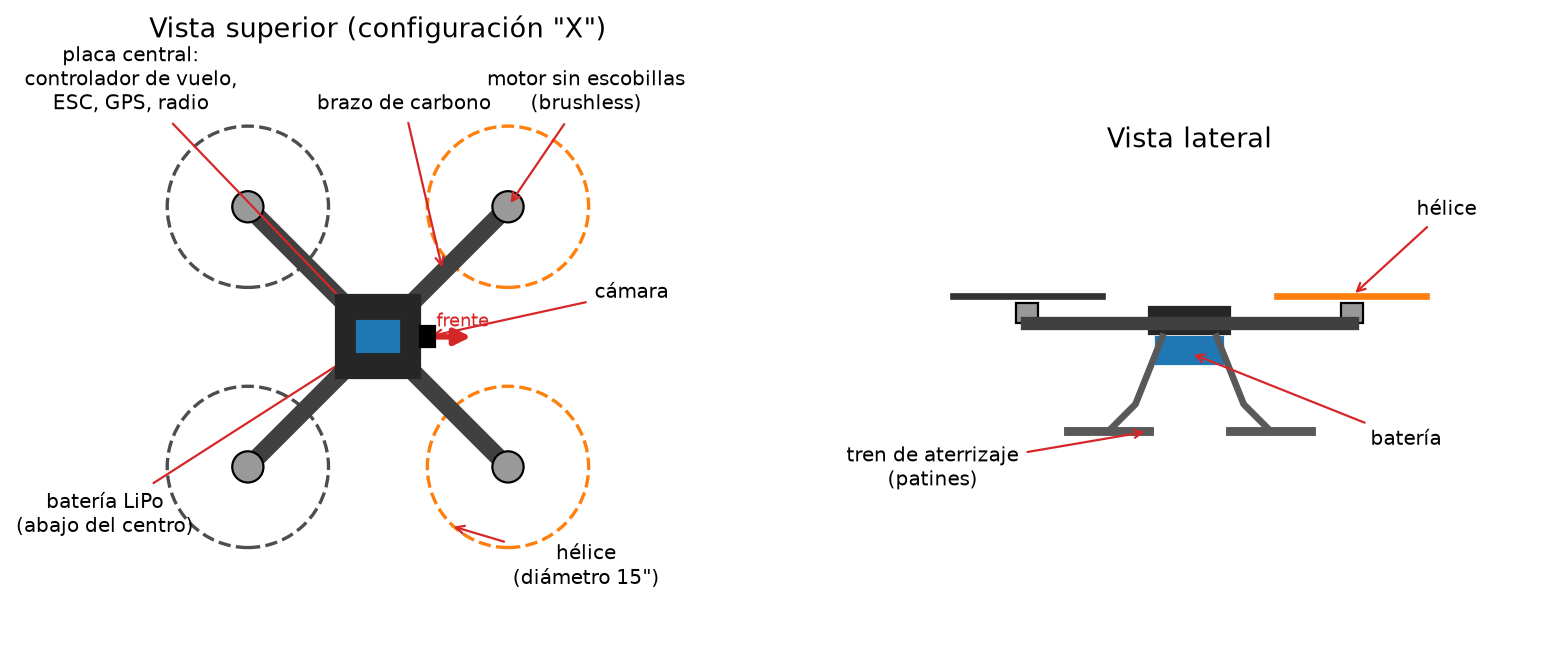
\includegraphics[width=\textwidth]{c_partes.png}
\caption{Partes de un cuadrirrotor como el Tarot 650.}
\label{fig:partes}
\end{figure}

\begin{description}
  \item[Marco (frame).] La estructura: una placa central y cuatro brazos. En el Tarot son de fibra de
        carbono, ligera y rígida. Los brazos del Tarot se pueden plegar para transportarlo.
  \item[Motores sin escobillas (brushless).] Motores eléctricos trifásicos muy eficientes. En el Tarot
        se usan T-Motor MN3508. Su constante KV dice cuántas revoluciones por minuto da por cada volt.
  \item[ESC (controlador electrónico de velocidad).] Uno por motor. Recibe una orden (``gira a tanto'')
        y genera las corrientes trifásicas para lograrlo.
  \item[Hélices.] Convierten el giro en empuje. Se describen con dos números: diámetro y paso, en
        pulgadas. Las del Tarot son de $15\times5$: 15'' de diámetro (38~cm) y 5'' de paso (lo que
        avanzarían en una vuelta si se ``atornillaran'' en el aire).
  \item[Batería LiPo.] Polímero de litio: mucha energía para su peso. Se describen por el número de
        celdas en serie (4S, 6S: 3.7~V cada una) y su capacidad en mAh.
  \item[Controlador de vuelo.] La computadora a bordo: lee los sensores y decide la velocidad de cada
        motor cientos de veces por segundo. Puede llevar ArduPilot o PX4. En nuestra simulación ese
        papel lo hacen nuestros controladores en Python o ArduPilot en SITL.
  \item[Sensores.] IMU (acelerómetros y giroscopios: cómo se mueve y gira), barómetro (altura),
        magnetómetro (brújula), GPS (posición) y, según la misión, cámaras y LiDAR.
  \item[Tren de aterrizaje.] Patas o patines para posarse sin dañar la cámara ni la batería.
\end{description}

\section{¿Por qué vuela? El empuje}

Una hélice que gira empuja aire hacia abajo; por la tercera ley de Newton (acción y reacción), el
aire empuja a la hélice hacia arriba. A esa fuerza se le llama \textbf{empuje}. Crece con el
\emph{cuadrado} de la velocidad de giro: al doble de velocidad, cuatro veces más empuje.

\begin{figure}[H]
\centering
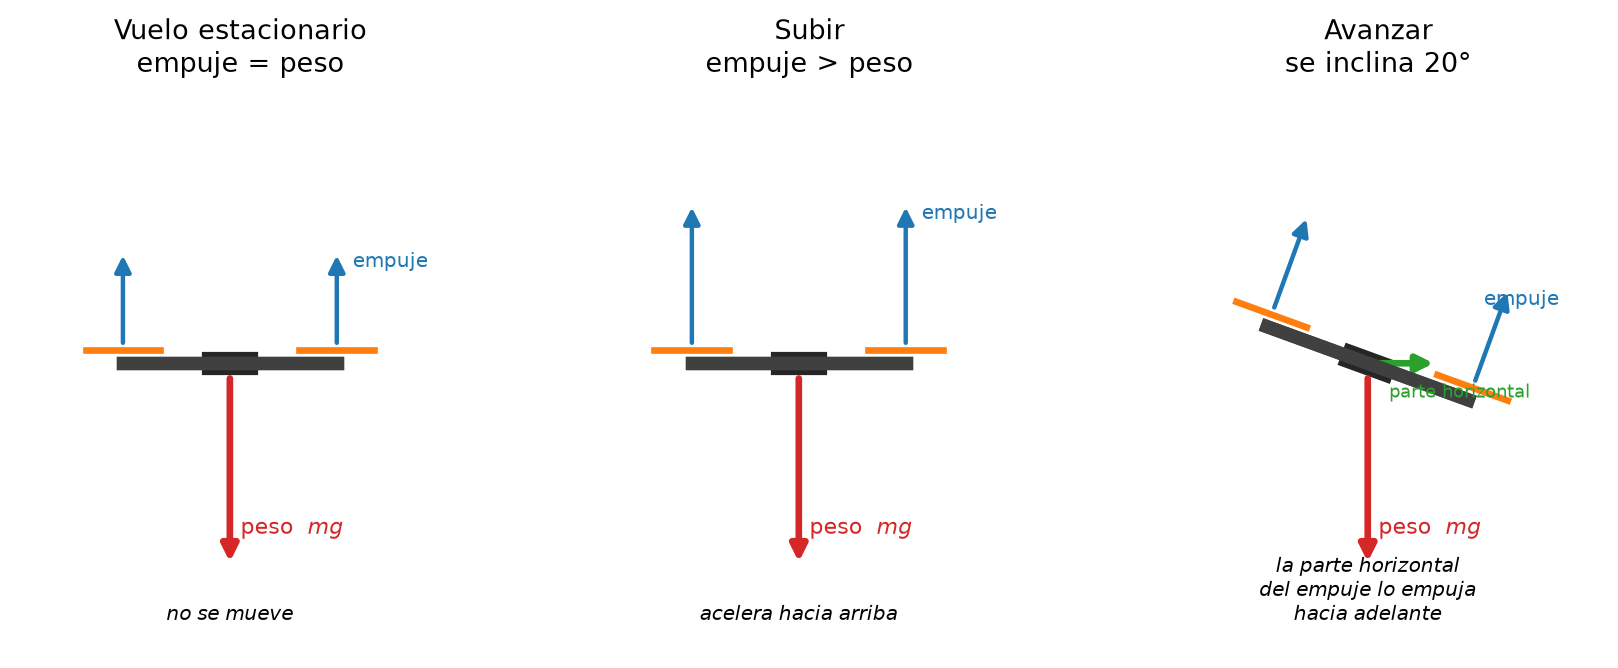
\includegraphics[width=\textwidth]{c_fuerzas.png}
\caption{Las dos fuerzas principales: el empuje de las hélices (azul) y el peso (rojo).}
\label{fig:fuerzas}
\end{figure}

\begin{itemize}
  \item Si el empuje total es igual al peso, el dron se queda quieto en el aire: \textbf{vuelo
        estacionario} (\emph{hover}).
  \item Si es mayor, sube; si es menor, baja.
  \item Para avanzar, el dron \textbf{se inclina}: el empuje ya no apunta hacia arriba, y su parte
        horizontal lo empuja hacia adelante (figura~\ref{fig:fuerzas}, derecha). Un cuadrirrotor no
        tiene ``motor hacia adelante'': avanza inclinándose, como una persona que se inclina para
        empezar a caminar.
\end{itemize}

\begin{ejemplo}
Sostén un libro con la mano extendida, plano. Para moverlo hacia adelante sin empujarlo, inclínalo un
poco: la fuerza de tu mano ``hacia arriba'' ahora tiene una parte hacia adelante. Así avanza un dron.
\end{ejemplo}

\section{Cómo se mueve: subir, alabeo, cabeceo y guiñada}

Un objeto en el espacio puede girar alrededor de tres ejes (figura~\ref{fig:ejes-c}). En aviación
esos giros tienen nombre:
\begin{description}
  \item[Alabeo (roll, $\phi$):] girar alrededor del eje que va al frente; el dron ``se ladea''.
  \item[Cabeceo (pitch, $\theta$):] girar alrededor del eje lateral; ``asiente con la cabeza''.
  \item[Guiñada (yaw, $\psi$):] girar alrededor del eje vertical; cambia hacia dónde mira.
\end{description}

\begin{figure}[H]
\centering
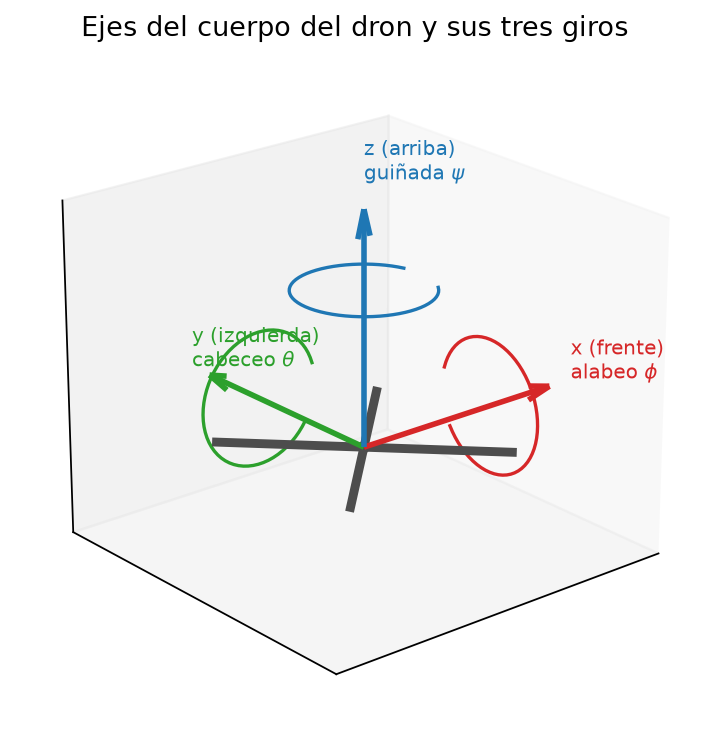
\includegraphics[width=0.6\textwidth]{c_ejes.png}
\caption{Ejes del cuerpo: \emph{x} al frente, \emph{y} a la izquierda, \emph{z} arriba.}
\label{fig:ejes-c}
\end{figure}

Con cuatro motores se controla todo así (figura~\ref{fig:movimientos}):

\begin{figure}[H]
\centering
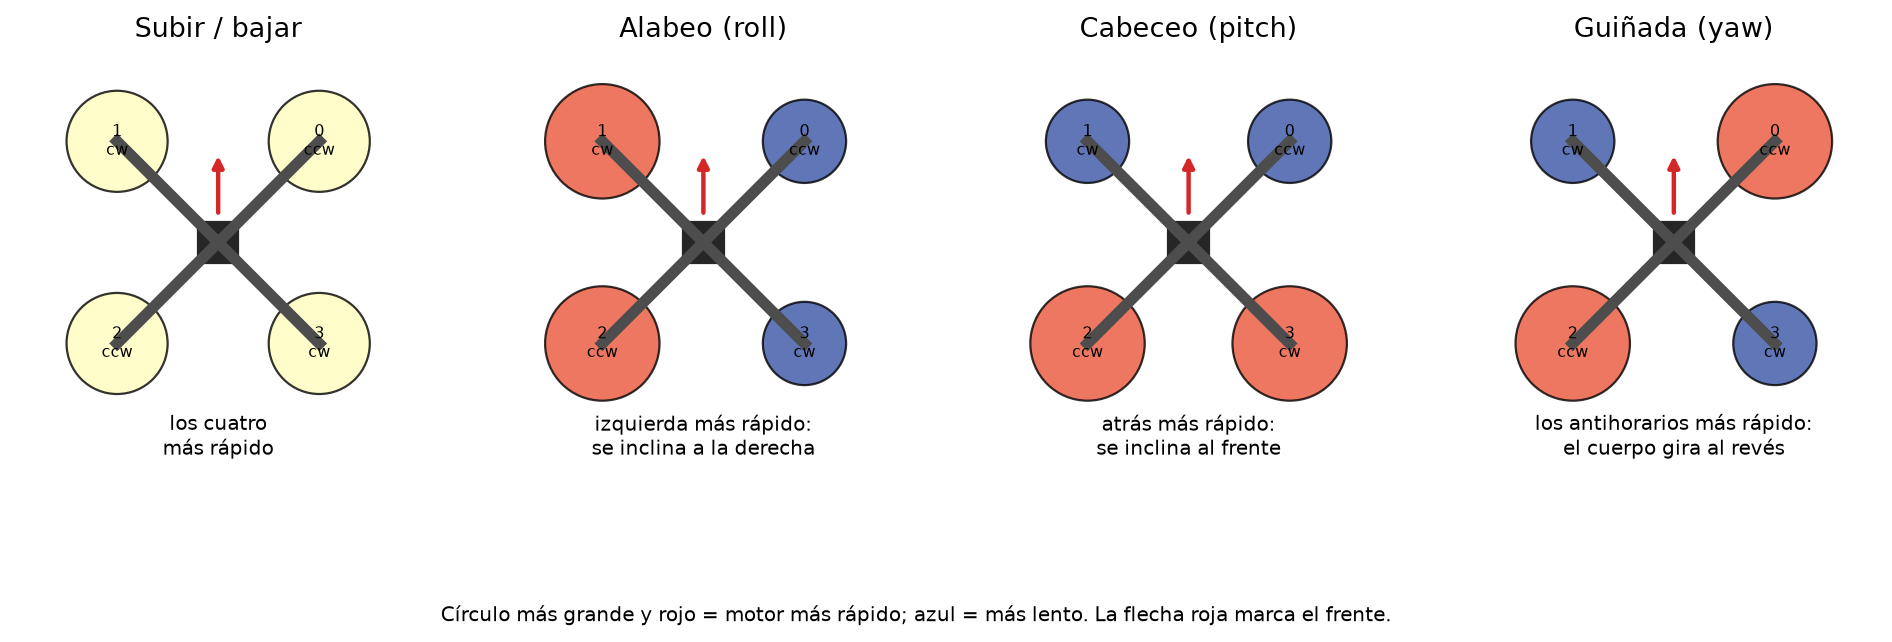
\includegraphics[width=\textwidth]{c_movimientos.png}
\caption{Cómo produce el dron cada movimiento solo cambiando la velocidad de los motores.}
\label{fig:movimientos}
\end{figure}

\begin{itemize}
  \item \textbf{Subir o bajar:} los cuatro motores aceleran o frenan por igual.
  \item \textbf{Alabeo:} los motores de un lado giran más rápido que los del otro; el dron se inclina
        hacia el lado lento y empieza a moverse de lado.
  \item \textbf{Cabeceo:} igual, pero adelante contra atrás; así avanza o retrocede.
  \item \textbf{Guiñada:} aquí entra un truco. Cada hélice, al girar, ``empuja'' el aire de lado y
        el aire, por reacción, intenta hacer girar al dron al revés. Por eso dos hélices giran en un
        sentido y dos en el otro: los efectos se cancelan. Si se aceleran las dos que giran en un
        sentido y se frenan las otras dos, el empuje total no cambia pero sobra par en un sentido, y
        el dron gira sobre sí mismo.
\end{itemize}

\begin{recuerda}
Cuatro motores, cuatro ``perillas'': empuje total, alabeo, cabeceo y guiñada. El avance y el
movimiento lateral no se controlan directamente: se consiguen inclinando el dron. Por eso el control
de un dron es \emph{en cascada}: para ir a una posición hay que pedir una inclinación, y para lograr
la inclinación hay que pedir velocidades a los motores.
\end{recuerda}

\section{Configuración ``+'' y ``X''}

Si un brazo apunta al frente, la configuración es ``+''; si el frente queda entre dos brazos, es
``X''. La ``X'' es la más común: la cámara frontal no ve hélices y los cuatro motores trabajan al
inclinarse hacia adelante. En la simulación hay un cuadrirrotor genérico en ``+'' y el Tarot en ``X''.

\section{El Tarot Ironman 650}

\begin{figure}[H]
\centering
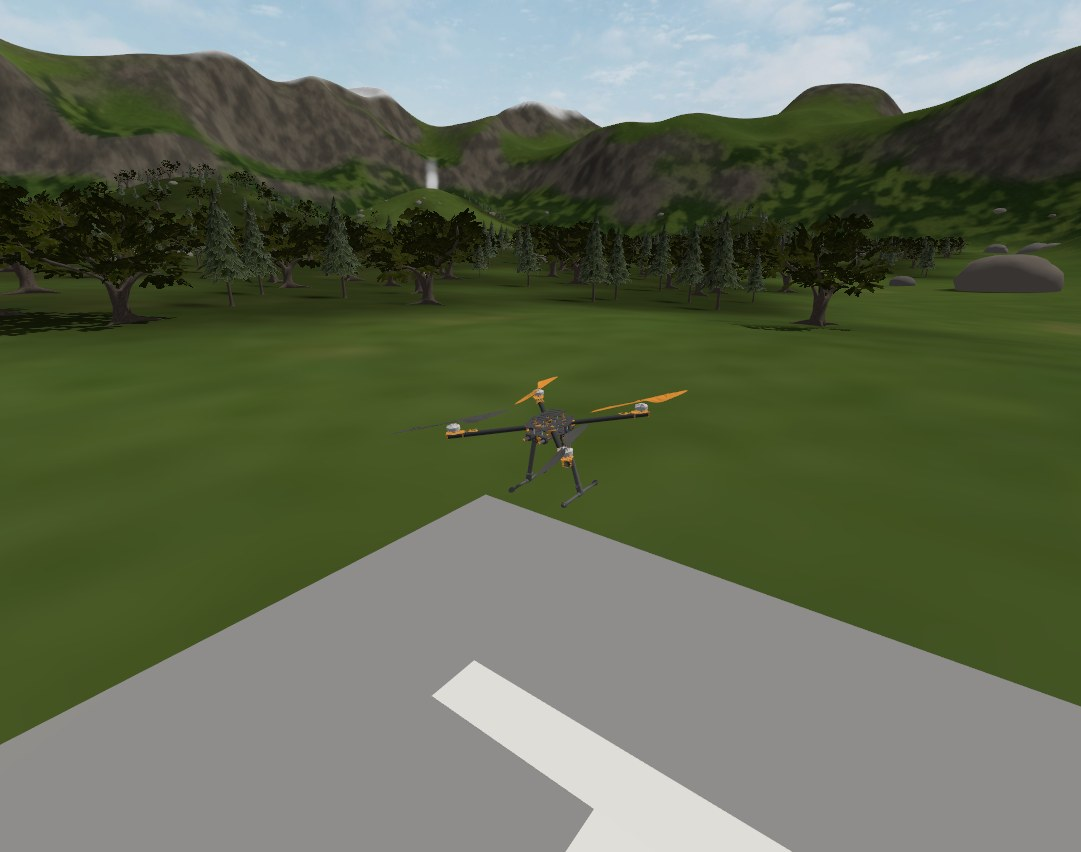
\includegraphics[width=0.8\textwidth]{gz_tarot_cerca.jpg}
\caption{El Tarot 650 simulado, en vuelo estacionario sobre su base.}
\end{figure}

El Tarot Ironman 650 es un marco comercial de fibra de carbono, muy usado en investigación porque
carga cámaras y computadoras sin problema. ``650'' es la distancia en milímetros entre motores
opuestos (en diagonal). Nuestro modelo:
\begin{itemize}
  \item motores a $(\pm0.22, \pm0.21)$~m del centro, en ``X'';
  \item hélices de 15'';
  \item 2.2~kg de masa total (supuesto);
  \item cada motor da hasta $\approx$19.6~N (unos 2~kg) de empuje: en total puede levantar
        $\approx$3.6 veces su peso. Esa \textbf{relación empuje/peso} da margen para maniobrar y
        resistir el viento.
\end{itemize}

\begin{tecnico}
En vuelo estacionario cada motor sostiene un cuarto del peso: $2.2\times9.81/4 = 5.4$~N. Como el
empuje es $f = k_f\omega^2$, con $k_f = 4.24\times10^{-5}$ la velocidad necesaria es
$\omega = \sqrt{5.4/k_f} = 357$~rad/s, unas 3400 revoluciones por minuto.
\end{tecnico}

\section{Para qué sirve un dron en un incendio forestal}

Un incendio se combate mejor cuanto antes se detecta y cuanto mejor se conoce su ubicación. Un dron
puede recorrer zonas de difícil acceso, ver por encima de las copas, detectar el humo desde lejos,
dar las coordenadas exactas del foco y quedarse vigilándolo, sin poner en riesgo a un piloto. Para
hacerlo de forma autónoma necesita tres capacidades, que son las tres partes centrales del libro:
\begin{enumerate}
  \item \textbf{Control} preciso aunque haya viento (Parte~II);
  \item \textbf{percepción}: ver y reconocer el fuego (Parte~III);
  \item \textbf{autonomía}: decidir a dónde ir y qué hacer (Parte~V).
\end{enumerate}

\chapter{Física sin miedo}

\begin{enpocas}
Vectores, las leyes de Newton aplicadas al dron, por qué el empuje crece con el cuadrado de la
velocidad, qué es la inercia, qué son los marcos de referencia (ENU, NED, cuerpo) y cómo se describe
una rotación. Al final, las ecuaciones del dron en una sola página.
\end{enpocas}

\section{Vectores: flechas con tamaño y dirección}

Muchas cantidades físicas no son solo un número: la velocidad de un dron es ``5~m/s \emph{hacia el
norte}''. Esas cantidades se llaman \textbf{vectores} y se dibujan como flechas. En tres
dimensiones un vector tiene tres componentes, por ejemplo $v = (v_x, v_y, v_z)$. Posición,
velocidad, aceleración, fuerza y velocidad angular son vectores.

\section{Las leyes de Newton aplicadas al dron}

\begin{enumerate}
  \item \textbf{Inercia.} Un cuerpo sigue como está (quieto o moviéndose en línea recta) mientras
        nadie lo empuje. Un dron que avanza y apaga la inclinación sigue avanzando un rato.
  \item \textbf{$F = ma$.} La aceleración es la fuerza total dividida entre la masa. Para el dron:
        \begin{equation}
        m\,\ddot p = \underbrace{T\,R\,e_3}_{\text{empuje}} \;\underbrace{-\,mg\,e_3}_{\text{peso}} \;+\; \underbrace{d(t)}_{\text{viento}}
        \end{equation}
        donde $\ddot p$ es la aceleración, $T$ el empuje total, $R e_3$ la dirección ``arriba'' del
        dron (que cambia si se inclina) y $e_3 = (0,0,1)$ la vertical.
  \item \textbf{Acción y reacción.} La hélice empuja aire hacia abajo y el aire empuja la hélice
        hacia arriba. También explica la guiñada: al hacer girar la hélice, el motor ``empuja'' al
        dron en sentido contrario.
\end{enumerate}

\section{Empuje: el cuadrado de la velocidad}

\begin{figure}[H]
\centering
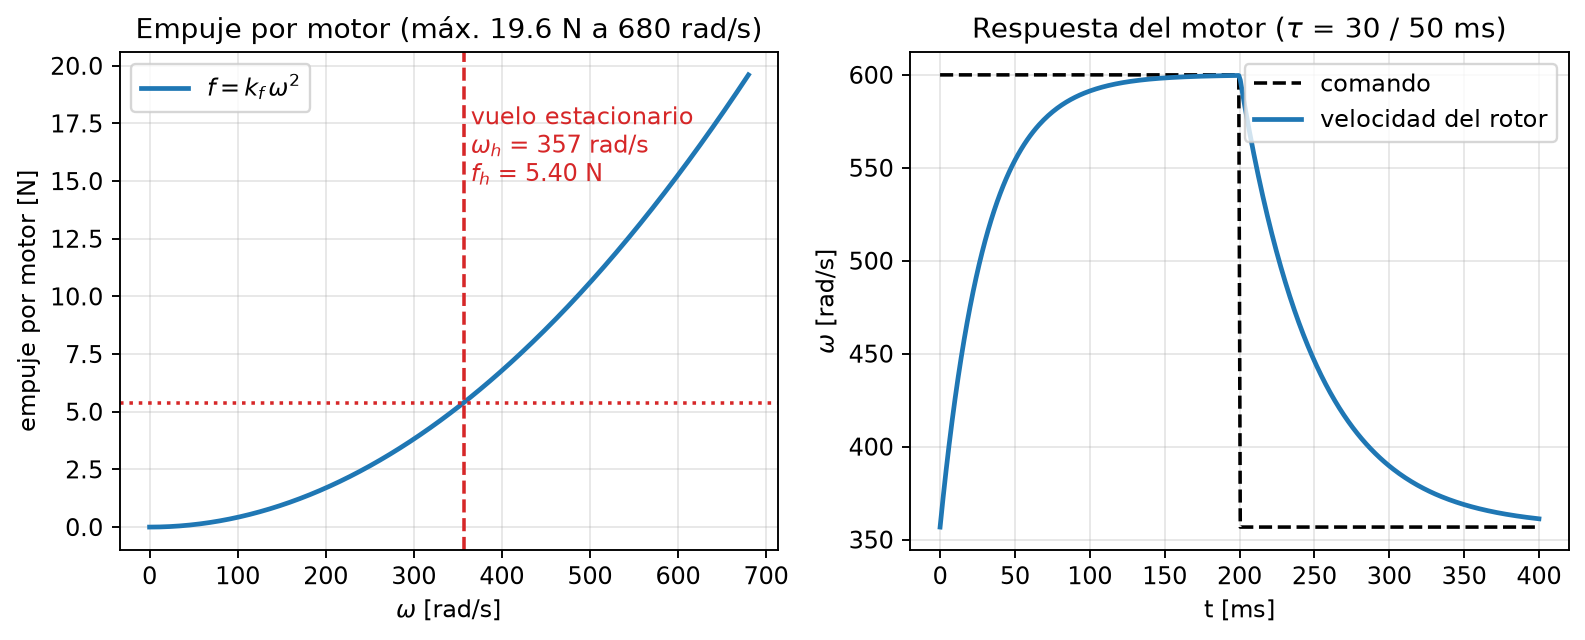
\includegraphics[width=\textwidth]{motor_empuje.png}
\caption{Izquierda: el empuje de un motor del Tarot crece como $\omega^2$. Derecha: el motor no
cambia de velocidad al instante, tarda unos 30--50~ms.}
\label{fig:empuje-fisica}
\end{figure}

El empuje de una hélice es aproximadamente
\begin{equation}
f = k_f\,\omega^2 ,
\end{equation}
con $\omega$ la velocidad de giro en rad/s y $k_f$ una constante que depende de la hélice y del aire.
Que sea cuadrático tiene consecuencias: cerca del vuelo estacionario un pequeño cambio de velocidad da
un cambio de empuje más o menos proporcional, pero no hay una relación lineal en todo el rango, y el
controlador tiene que tenerlo en cuenta (por eso calcula fuerzas y luego saca raíces cuadradas para
obtener velocidades).

Además del empuje, cada hélice produce un \textbf{par de arrastre} (una ``torsión'') proporcional a
su empuje, $k_m f$: es lo que intenta girar al dron al revés de la hélice.

\begin{recuerda}
Los motores no son instantáneos. En el Tarot simulado tardan $\approx$30~ms en acelerar y
$\approx$50~ms en frenar. Ese retardo es parte de lo que hace difícil el control, y tiene un papel
importante en los resultados del control.
\end{recuerda}

\section{Inercia de rotación y par}

Para girar, lo que importa no es la masa sino el \textbf{momento de inercia} $J$: cuánto se resiste
un cuerpo a cambiar su giro. Depende de cómo está repartida la masa: un patinador que encoge los
brazos gira más rápido porque baja su momento de inercia. El dron tiene un momento de inercia para
cada eje (en el Tarot: 0.034, 0.036 y 0.066~kg\,m$^2$; el del eje vertical es mayor porque los
motores están lejos del centro en ese plano).

Lo que hace girar es un \textbf{par} (o torque) $\tau$: una fuerza aplicada a cierta distancia del
centro. Un motor de un brazo que empuja más que el del brazo opuesto produce un par que ladea al dron.
La ``segunda ley de Newton para giros'' es
\begin{equation}
J\,\dot\omega = \tau - \omega\times J\omega .
\end{equation}
El último término es un efecto giroscópico; para entender la idea basta con ``par = inercia por
aceleración angular''.

\section{Marcos de referencia: ¿desde dónde mido?}

Decir ``el dron está en $(3, 5, 10)$'' no significa nada si no se dice desde dónde y con qué ejes.
Eso es un \textbf{marco de referencia}. En este proyecto aparecen tres:

\begin{description}
  \item[Mundo ENU] (Este, Norte, Arriba): fijo al suelo, con origen en el centro del mundo de Gazebo.
        Lo usan Gazebo y ROS.
  \item[Mundo NED] (Norte, Este, Abajo): el mismo lugar, pero con otros ejes. Lo usa la aviación y
        ArduPilot. Pasar de uno a otro es solo cambiar $x\leftrightarrow y$ y el signo de $z$.
  \item[Cuerpo:] pegado al dron y que se mueve con él: \emph{x} al frente, \emph{y} a la izquierda,
        \emph{z} arriba. Los sensores (IMU, cámara, LiDAR) miden en este marco.
\end{description}

\begin{figure}[H]
\centering
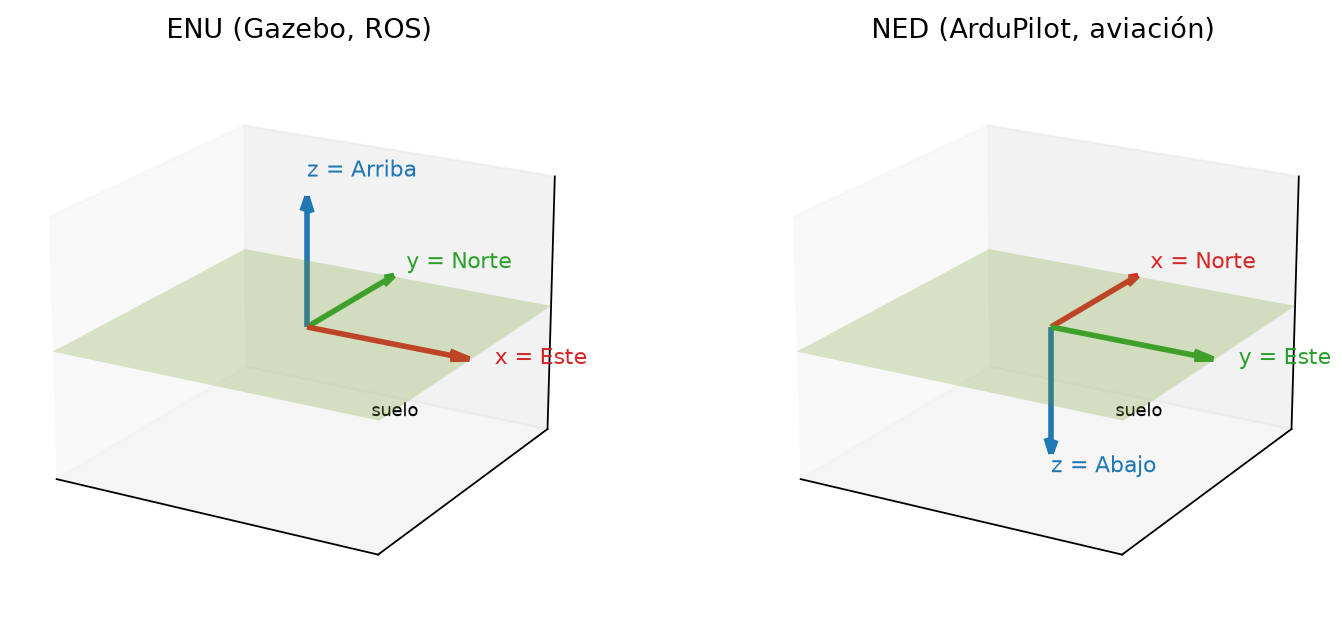
\includegraphics[width=0.9\textwidth]{c_marcos.png}
\caption{Los dos marcos del mundo. Confundirlos es una de las causas más comunes de errores en
drones.}
\end{figure}

\begin{figure}[H]
\centering
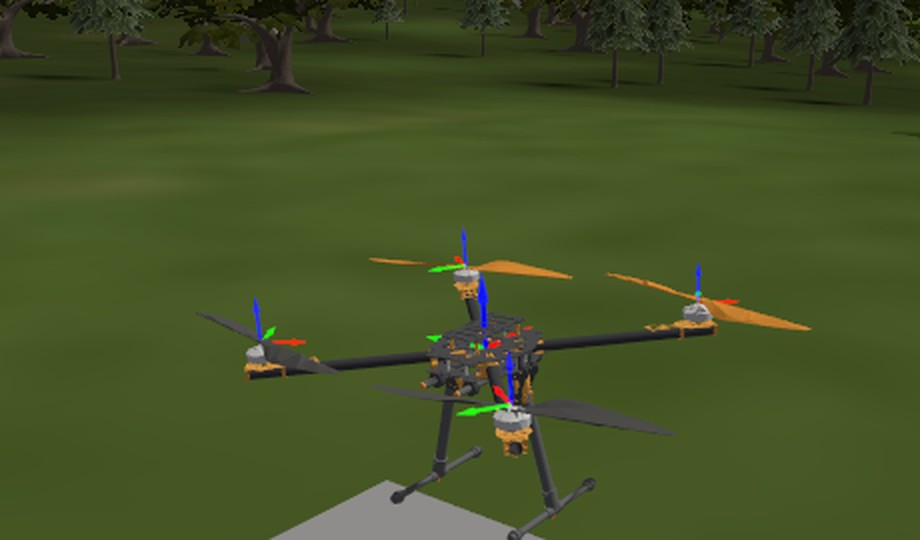
\includegraphics[width=0.6\textwidth]{gz_tarot_marcos.jpg}
\caption{En Gazebo se pueden mostrar los marcos de cada pieza del dron (rojo = \emph{x},
verde = \emph{y}, azul = \emph{z}).}
\end{figure}

\begin{leccion}
Durante el desarrollo, el vuelo con ArduPilot mandaba al dron 330~m lejos de donde debía ir: se
restaba dos veces la posición de salida al pasar del marco del mundo al marco local de ArduPilot. El
dron llegó a estrellarse contra un cerro. Se arregló midiendo el desfase entre los dos marcos en
lugar de suponerlo (sección~\ref{sec:plugin-ap}). Moraleja: \textbf{siempre verifica en qué marco
está cada número}.
\end{leccion}

\section{Rotaciones y ángulos de Euler}

La orientación del dron se puede describir con tres ángulos, alabeo $\phi$, cabeceo $\theta$ y
guiñada $\psi$ (los \textbf{ángulos de Euler}), aplicados en cierto orden. Para hacer cuentas es más
cómodo una \textbf{matriz de rotación} $R$ de $3\times3$: sus tres columnas son los ejes del dron
vistos desde el mundo. Multiplicar un vector del cuerpo por $R$ lo ``pasa'' al mundo. Por ejemplo,
la dirección del empuje es la tercera columna de $R$, $R e_3$.

\begin{tecnico}
Gazebo y ROS entregan la orientación como un \textbf{cuaternión} $(q_x, q_y, q_z, q_w)$: cuatro
números que representan una rotación sin las singularidades de los ángulos de Euler (que fallan
cuando el cabeceo llega a 90°). El código convierte cuaterniones a matrices con
\cod{dinamica.quat_a_rot}.
\end{tecnico}

\section{Las ecuaciones del dron en una página}

\begin{tcolorbox}[colback=white,colframe=NavyBlue!60!black,title=Modelo del cuadrirrotor]
\begin{align*}
\text{posición:}\quad & m\ddot p = T R e_3 - mg\,e_3 + d(t)\\
\text{orientación:}\quad & \dot R = R\hat\omega\\
\text{giro:}\quad & J\dot\omega = \tau - \omega\times J\omega\\
\text{motores:}\quad & f_i = k_f\omega_i^2,\qquad T = \textstyle\sum_i f_i,\qquad
\tau = \big(\textstyle\sum y_i f_i,\ -\sum x_i f_i,\ -\sum s_i k_m f_i\big)
\end{align*}
\end{tcolorbox}

No hace falta resolverlas a mano: Gazebo las integra por nosotros (Capítulo~\ref{cap:simulacion}).
Pero el controlador las usa para saber cuánto empuje y cuánto par pedir.

\chapter{¿Qué es una simulación? Gazebo}
\label{cap:simulacion}

\begin{enpocas}
Por qué se simula antes de volar, qué hace un simulador de robots como Gazebo, cómo se describe un
robot (SDF), la diferencia entre lo que se ve y lo que choca, qué son los \emph{plugins} y qué
significan SITL y ``factor de tiempo real''.
\end{enpocas}

\section{¿Por qué simular?}

Un Tarot 650 con cámara cuesta varios miles de pesos y un error de programación puede estrellarlo en
segundos. Además, para probar la búsqueda de un incendio harían falta un bosque, un incendio y
permisos. Un simulador resuelve todo eso:
\begin{itemize}
  \item los choques son gratis: se reinicia y listo;
  \item se puede repetir exactamente el mismo experimento (mismo viento, mismo incendio) para comparar
        controladores, algo imposible al aire libre;
  \item se puede medir todo, incluida la posición \emph{verdadera} del dron, que en la vida real nunca
        se conoce exactamente;
  \item se puede acelerar o pausar el tiempo.
\end{itemize}
A cambio, un simulador es una aproximación: el viento, la aerodinámica o la cámara nunca son
idénticos a los reales. Por eso el camino es simular, luego volar con cuidado y comparar.

\begin{recuerda}
La simulación no reemplaza el vuelo real: lo prepara. Lo que no funciona en simulación, casi seguro
no funcionará en el dron; lo que funciona en simulación, probablemente funcionará con ajustes.
\end{recuerda}

\section{Gazebo}

\textbf{Gazebo} (en su versión \emph{Harmonic}) es un simulador de robots de código abierto. En cada
paso de tiempo (1~ms en nuestro caso):
\begin{enumerate}
  \item un \textbf{motor de física} (DART) calcula fuerzas, contactos y movimientos de todos los
        cuerpos, resolviendo ecuaciones como las del capítulo anterior;
  \item un \textbf{motor de render} (OGRE 2) dibuja la escena en 3D, lo que permite simular cámaras y
        LiDAR;
  \item los \textbf{sensores} simulados (IMU, cámara, LiDAR, odometría) generan sus mediciones;
  \item los \textbf{plugins} (pequeños programas) agregan comportamientos: motores, viento, partículas
        de fuego, conexión con ArduPilot.
\end{enumerate}

\begin{figure}[H]
\centering
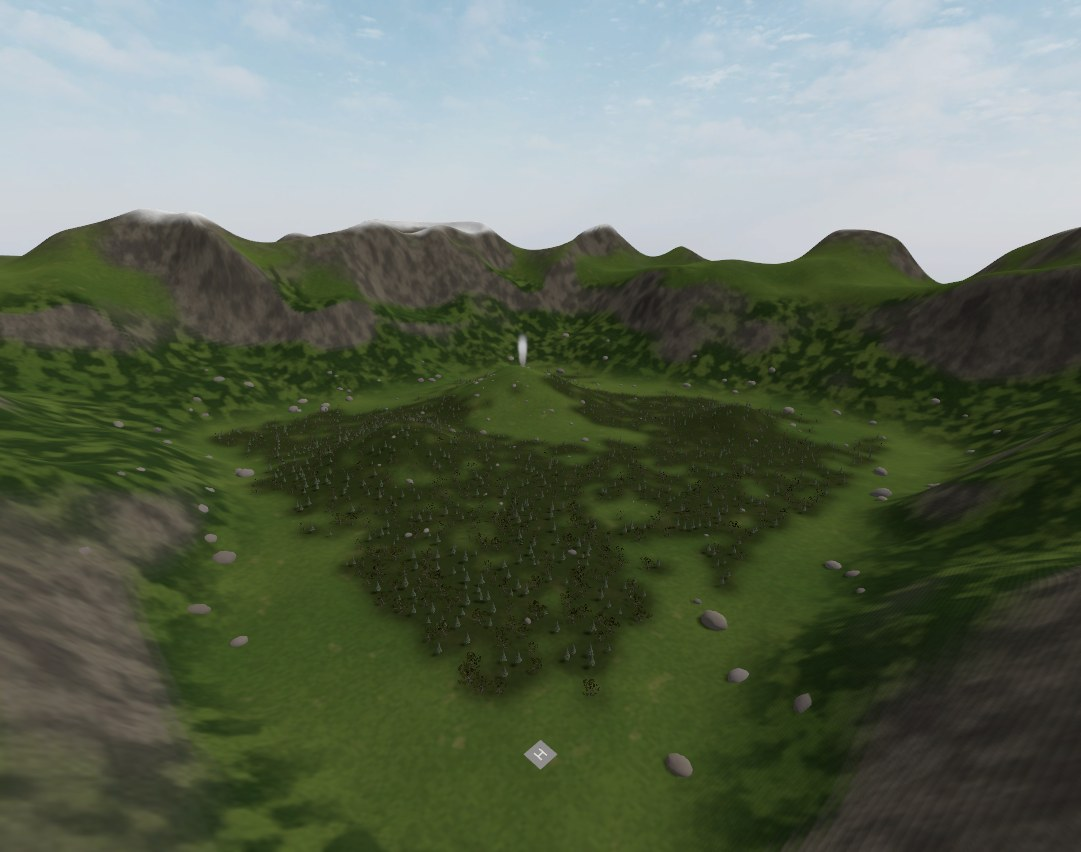
\includegraphics[width=\textwidth]{gz_valle_aereo.jpg}
\caption{El mundo \cod{bosque_grande} visto en Gazebo: terreno, árboles, rocas, cielo y, al fondo, el
humo del incendio.}
\end{figure}

\section{Cómo se describe un robot: SDF}

Gazebo lee los robots y los mundos en archivos \textbf{SDF} (\emph{Simulation Description Format}),
que son texto en formato XML. Un robot se describe con:
\begin{description}
  \item[Eslabones (\emph{links}):] piezas rígidas, cada una con masa, inercia, una forma para dibujar
        y otra para chocar. El Tarot tiene el cuerpo y cuatro rotores.
  \item[Articulaciones (\emph{joints}):] cómo se unen los eslabones; los rotores giran respecto al
        cuerpo en articulaciones \emph{revolute}.
  \item[Sensores] montados en un eslabón, con su posición y orientación.
  \item[Plugins] que les dan vida.
\end{description}

Un fragmento simplificado:
\begin{lstlisting}[style=xml]
<model name="cuadrirotor">
  <link name="base_link">
    <inertial><mass>2.12</mass> ... </inertial>
    <visual name="placas"> <geometry><mesh><uri>model://tarot650/meshes/placas.stl</uri></mesh></geometry> </visual>
    <collision name="cuerpo_col"> <geometry><box><size>0.16 0.16 0.06</size></box></geometry> </collision>
    <sensor name="camara" type="camera"> ... </sensor>
  </link>
  <link name="rotor_0"> ... </link>
  <joint name="rotor_0_joint" type="revolute"> <parent>base_link</parent> <child>rotor_0</child> ... </joint>
  <plugin filename="gz-sim-multicopter-motor-model-system" ...> ... </plugin>
</model>
\end{lstlisting}

\section{Lo que se ve y lo que choca}

Cada eslabón tiene dos formas. La \textbf{visual} es la que se dibuja: puede ser una malla 3D muy
detallada, como la del CAD del Tarot. La de \textbf{colisión} es la que usa la física para detectar
choques: conviene que sea simple (cajas, cilindros) porque calcular contactos entre mallas
complicadas es lento y frágil.

\begin{figure}[H]
\centering
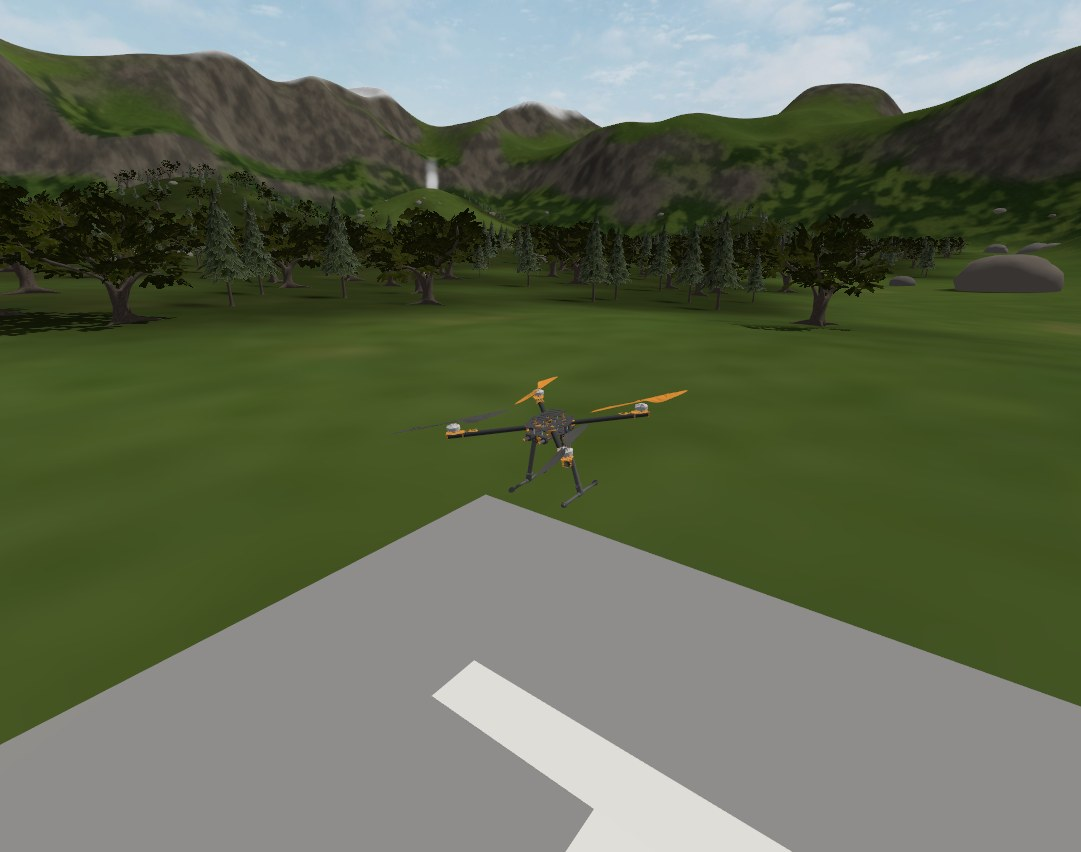
\includegraphics[width=0.48\textwidth]{gz_tarot_cerca.jpg}\hfill
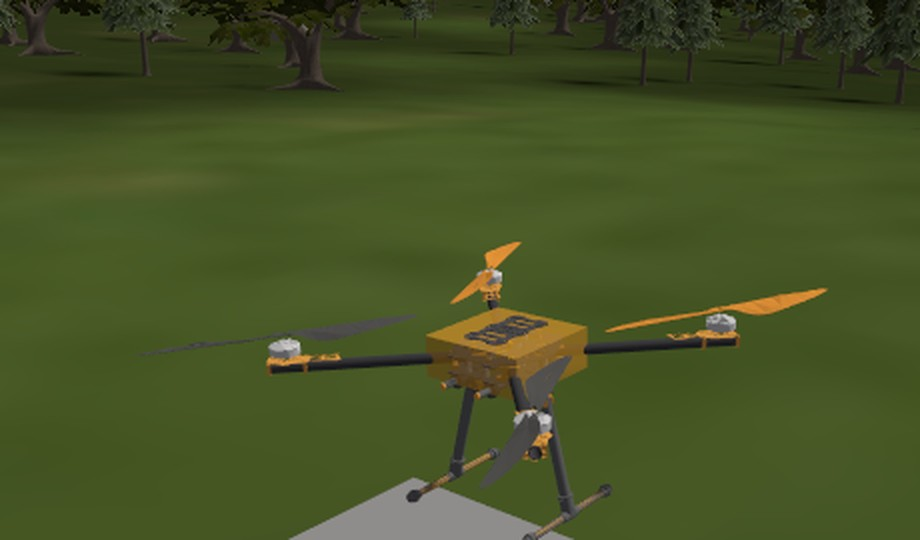
\includegraphics[width=0.48\textwidth]{gz_tarot_colisiones.jpg}
\caption{Izquierda: la forma visual del Tarot. Derecha: Gazebo mostrando sus formas de colisión (en
naranja): una caja para el cuerpo y dos cilindros delgados para los patines.}
\end{figure}

\begin{leccion}
En el mundo grande, las rocas usaban como colisión mallas OBJ sin \emph{normales} (los vectores que
dicen hacia dónde ``mira'' cada triángulo). Gazebo se caía con un \emph{segfault} en cuanto algo las
tocaba. Exportarlas con normales lo arregló.
\end{leccion}

\section{Plugins}

Un \emph{plugin} es código (en C++) que Gazebo carga para agregar un comportamiento. En este proyecto
se usan:
\begin{description}
  \item[\cod{MulticopterMotorModel}] (de Gazebo): convierte una velocidad pedida en empuje y par de un
        rotor, con su retardo.
  \item[\cod{OdometryPublisher}:] publica la posición y velocidad verdaderas del dron.
  \item[\cod{ParticleEmitter}:] las llamas y el humo.
  \item[\cod{FuerzaViento}] (nuestro): aplica la fuerza del viento.
  \item[\cod{ComandosMotores}] (nuestro) y \cod{ArduPilotPlugin}: para volar con ArduPilot.
\end{description}

\section{Tiempo simulado y factor de tiempo real}

La simulación tiene su propio reloj. Si la computadora es rápida, un segundo simulado tarda un segundo
real; si no, tarda más. El \textbf{factor de tiempo real} (RTF) es la razón entre los dos: RTF = 1
significa tiempo real; RTF = 0.5, que todo va a la mitad de velocidad. Con la RTX 5060 Ti el mundo
grande corre a RTF $\approx$1.0 (0.8 con el LiDAR). Todos los nodos usan el reloj simulado
(\cod{use_sim_time}), así que los resultados no dependen de la velocidad de la computadora.

\section{SITL y HITL}

\begin{description}
  \item[SITL] (\emph{software in the loop}): el mismo programa del piloto automático que volaría en el
        dron (aquí ArduCopter) corre en la computadora y ``vuela'' el dron simulado. Es lo que hacemos
        en el capítulo~\ref{cap:autopiloto}.
  \item[HITL] (\emph{hardware in the loop}): el controlador de vuelo físico está conectado a la
        simulación. Es el paso siguiente antes de volar.
\end{description}

\begin{ejercicio}
Lanza la simulación (capítulo~\ref{cap:primer-vuelo}) y, en la ventana de Gazebo, haz clic derecho
sobre el dron $\rightarrow$ \emph{View} $\rightarrow$ \emph{Collisions}. Verás las formas de choque.
Prueba también \emph{Inertia} y \emph{Frames}.
\end{ejercicio}

\chapter{ROS 2 para principiantes}

\begin{enpocas}
Qué es ROS~2, la terminal en cinco minutos, nodos, tópicos, mensajes, servicios, parámetros,
archivos \emph{launch} y el espacio de trabajo. Con ejemplos de nuestra simulación.
\end{enpocas}

\section{La terminal en cinco minutos}

Casi todo se hace escribiendo órdenes en una \textbf{terminal} (Ctrl+Alt+T en Ubuntu). Lo mínimo:

\begin{lstlisting}[style=bash]
pwd                      # ¿en qué carpeta estoy?
ls                       # ¿qué hay aquí?
cd ~/ros2_ws             # entrar a una carpeta (~ es tu carpeta personal)
cd ..                    # subir un nivel
cat archivo.txt          # ver un archivo
nano archivo.txt         # editar un archivo (Ctrl+O guarda, Ctrl+X sale)
Ctrl+C                   # detener el programa que está corriendo
\end{lstlisting}

\begin{consejo}
La tecla Tab completa nombres de archivos y órdenes; la flecha hacia arriba recupera la orden
anterior. Ahorran muchísimo tiempo y errores de dedo.
\end{consejo}

\section{¿Qué es ROS 2?}

\textbf{ROS} (\emph{Robot Operating System}) no es un sistema operativo: es un conjunto de
herramientas para que muchos programas pequeños de un robot hablen entre sí. En lugar de un programa
gigante que lo hace todo, hay un programa que lee la cámara, otro que detecta fuego, otro que decide
a dónde ir, otro que controla los motores... y ROS los conecta. Usamos la versión \textbf{ROS~2
Jazzy}.

\begin{ejemplo}
Piensa en una cocina de restaurante. El que recibe pedidos los pega en un tablero; el cocinero toma
los pedidos del tablero; el mesero recoge los platos de la barra. Nadie habla directamente con nadie:
todos leen y escriben en lugares comunes. En ROS, los cocineros son los \emph{nodos} y los tableros
son los \emph{tópicos}.
\end{ejemplo}

\section{Nodos, tópicos y mensajes}

\begin{description}
  \item[Nodo:] un programa que hace una tarea. En nuestra simulación: \cod{detector_yolo},
        \cod{busqueda_incendio}, \cod{controlador_sta}, \cod{viento}...
  \item[Tópico:] un canal con nombre por donde viajan datos, por ejemplo \cod{/cuadrirotor/camara}.
  \item[Mensaje:] el dato que viaja, con un tipo definido. \cod{sensor_msgs/Image} es una imagen;
        \cod{nav_msgs/Odometry}, una posición con velocidad.
  \item[Publicar / suscribirse:] un nodo \emph{publica} en un tópico y cualquier otro se
        \emph{suscribe} para recibir. El que publica no sabe quién escucha.
\end{description}

\begin{figure}[H]
\centering
\begin{tikzpicture}[
  nodo/.style={draw,ellipse,fill=green!12,minimum width=2.8cm,minimum height=0.9cm,font=\small},
  top/.style={draw,rectangle,fill=yellow!20,minimum width=3.2cm,minimum height=0.7cm,font=\scriptsize\ttfamily},
  fl/.style={-{Stealth[length=2.2mm]},thick}]
  \node[nodo] (gz) at (0,0) {Gazebo + puente};
  \node[top] (cam) at (4.2,0.8) {/cuadrirotor/camara};
  \node[top] (odo) at (4.2,-0.8) {/cuadrirotor/odometria};
  \node[nodo] (det) at (8.6,0.8) {detector\_yolo};
  \node[top] (detc) at (8.6,-1.0) {/cuadrirotor/detecciones};
  \node[nodo] (bus) at (8.6,-2.8) {busqueda\_incendio};
  \node[top] (con) at (4.2,-2.8) {/cuadrirotor/consigna};
  \node[nodo] (ctl) at (0,-2.8) {controlador\_sta};
  \draw[fl] (gz) -- (cam); \draw[fl] (gz) -- (odo); \draw[fl] (cam) -- (det);
  \draw[fl] (det) -- (detc); \draw[fl] (detc) -- (bus); \draw[fl] (odo) -- (bus);
  \draw[fl] (bus) -- (con); \draw[fl] (con) -- (ctl); \draw[fl] (odo) -- (ctl);
  \draw[fl] (ctl) -- node[left,font=\scriptsize]{/cuadrirotor/motores} (gz);
\end{tikzpicture}
\caption{Nodos (óvalos verdes) que se comunican por tópicos (rectángulos amarillos) en la misión de
búsqueda.}
\end{figure}

Para mirar desde la terminal:
\begin{lstlisting}[style=bash]
ros2 node list                                   # nodos que están corriendo
ros2 topic list                                  # tópicos que existen
ros2 topic echo /cuadrirotor/busqueda/estado     # ver lo que pasa por un tópico
ros2 topic hz /cuadrirotor/camara                # ¿cuántos mensajes por segundo?
ros2 topic info /cuadrirotor/odometria           # tipo y quién publica/escucha
ros2 interface show nav_msgs/msg/Odometry        # ¿qué campos tiene un mensaje?
\end{lstlisting}

\section{Servicios y parámetros}

\begin{description}
  \item[Servicio:] una pregunta con respuesta (como una llamada telefónica), a diferencia del tópico,
        que es una transmisión continua. El \emph{launch} usa servicios de Gazebo para hacer que la
        cámara de la ventana siga al dron.
  \item[Parámetro:] un ajuste de un nodo, como la altura de búsqueda o la ganancia del controlador.
        Se guardan en archivos \textbf{YAML}:
\end{description}
\begin{lstlisting}
busqueda_incendio:
  ros__parameters:
    altura_busqueda: 30.0     # metros sobre el suelo
    velocidad: 5.0            # m/s
\end{lstlisting}

\section{Archivos launch}

Arrancar diez nodos a mano sería tedioso. Un archivo \textbf{launch} (en Python) los arranca todos
con sus parámetros. El nuestro es \cod{launch/simulacion.launch.py} y recibe \emph{argumentos} para
elegir vehículo, mundo, controlador y misión:
\begin{lstlisting}[style=bash]
ros2 launch cuadrirotor_sim simulacion.launch.py vehiculo:=tarot650 mundo:=bosque_grande controlador:=sta mision:=busqueda
\end{lstlisting}

\section{El puente entre Gazebo y ROS}

Gazebo tiene su propio sistema de mensajes (\emph{gz-transport}). El nodo \cod{ros_gz_bridge}
traduce entre los dos mundos según la lista de \cod{config/puente.yaml}: la cámara, la odometría, la
IMU y el LiDAR van de Gazebo a ROS; las velocidades de los motores y el viento, de ROS a Gazebo.

\section{Paquetes y espacio de trabajo}

El código de ROS se organiza en \textbf{paquetes} (carpetas con un \cod{package.xml}). Los paquetes
viven en un \textbf{espacio de trabajo} (\emph{workspace}); el nuestro es \cod{~/ros2_ws}. Se
compila con \cod{colcon} y, antes de usarlo en cada terminal, se ``activa'' con \cod{source}:

\begin{lstlisting}[style=bash]
cd ~/ros2_ws
colcon build --symlink-install       # compila todos los paquetes de src/
source install/setup.bash            # hace visibles los paquetes en esta terminal
\end{lstlisting}

\begin{aviso}
Si una orden de ROS dice que no encuentra el paquete \cod{cuadrirotor_sim}, casi siempre es porque
olvidaste el \cod{source install/setup.bash} en esa terminal. Para no olvidarlo, agrégalo a
\cod{~/.bashrc}.
\end{aviso}

\begin{ejercicio}
Con la simulación corriendo, abre otra terminal, haz \cod{source} y escribe
\cod{ros2 topic echo /cuadrirotor/odometria --field pose.pose.position}. Verás la posición del dron
cambiar en tiempo real.
\end{ejercicio}


\part{El control: mantener el dron donde queremos}
\chapter{Control automático desde cero}

\begin{enpocas}
Qué es controlar, la diferencia entre lazo abierto y lazo cerrado, el error, los controladores P, PD
y PID, cómo se lee una respuesta y por qué un dron necesita control en cascada.
\end{enpocas}

\section{¿Qué es controlar?}

Controlar es conseguir que algo se comporte como queremos aunque haya perturbaciones. Queremos que el
dron esté a 30~m de altura; el viento lo empuja hacia abajo; el controlador acelera los motores para
compensar. Al ``algo'' que se controla se le llama \textbf{planta} (aquí, el dron); a lo que queremos,
\textbf{referencia} o \textbf{consigna}; a lo que nos estorba, \textbf{perturbación}.

\section{Lazo abierto y lazo cerrado}

\begin{figure}[H]
\centering
\begin{tikzpicture}[blq/.style={draw,rounded corners,fill=#1,minimum width=2.4cm,minimum height=0.9cm,align=center,font=\small},blq/.default=white,
  fl/.style={-{Stealth[length=2.2mm]},thick}, sum/.style={draw,circle,inner sep=1.5pt}]
  \node at (-1.4,0.9) {\textbf{Lazo abierto}};
  \node (r1) at (-1.2,0) {referencia};
  \node[blq=blue!10] (c1) at (2,0) {controlador};
  \node[blq=orange!15] (p1) at (5.5,0) {planta\\(dron)};
  \node (y1) at (8.6,0) {salida};
  \draw[fl] (r1) -- (c1); \draw[fl] (c1) -- node[above,font=\scriptsize]{acción} (p1); \draw[fl] (p1) -- (y1);
  \node (d1) at (5.5,1.3) {perturbación}; \draw[fl] (d1) -- (p1);

  \node at (-1.4,-1.7) {\textbf{Lazo cerrado}};
  \node (r2) at (-1.2,-2.6) {referencia};
  \node[sum] (s) at (0.5,-2.6) {$-$};
  \node[blq=blue!10] (c2) at (2.6,-2.6) {controlador};
  \node[blq=orange!15] (p2) at (5.9,-2.6) {planta\\(dron)};
  \node (y2) at (9,-2.6) {salida};
  \node[blq=green!12] (sen) at (5.9,-4.1) {sensor};
  \draw[fl] (r2) -- (s); \draw[fl] (s) -- node[above,font=\scriptsize]{error} (c2); \draw[fl] (c2) -- node[above,font=\scriptsize]{acción} (p2);
  \draw[fl] (p2) -- (y2); \draw[fl] (8.1,-2.6) |- (sen); \draw[fl] (sen) -| (s);
  \node (d2) at (5.9,-1.3) {perturbación}; \draw[fl] (d2) -- (p2);
\end{tikzpicture}
\caption{En lazo abierto se actúa ``a ciegas''. En lazo cerrado se mide el resultado, se compara con
lo que se quiere y se corrige: eso es la \emph{retroalimentación}.}
\end{figure}

\begin{ejemplo}
Una tostadora es lazo abierto: tuesta un tiempo fijo, aunque el pan se queme. Ajustar la temperatura
de la regadera es lazo cerrado: sientes el agua (sensor), la comparas con la que quieres (error) y
mueves la llave (acción). Si alguien abre otra llave en la casa (perturbación), lo notas y corriges.
\end{ejemplo}

Un dron sin lazo cerrado no se puede volar: cualquier ráfaga o diferencia entre motores lo voltea
en un segundo. El \textbf{error} es la diferencia entre lo que queremos y lo que hay,
$e = \text{referencia} - \text{medición}$, y todo controlador hace algo con él.

\section{El controlador proporcional (P)}

La idea más simple: actuar en proporción al error. Si estoy 2~m abajo, empujo el doble que si estoy
1~m abajo:
\begin{equation}
u = K_p\, e .
\end{equation}
$K_p$ es la \textbf{ganancia proporcional}. El problema con un dron: el control P actúa sobre la
\emph{aceleración}, y un objeto que se acelera hacia el objetivo llega con velocidad, se pasa,
regresa, se vuelve a pasar... oscila para siempre (curva gris de la figura~\ref{fig:pid}).

\section{El término derivativo (D): frenar a tiempo}

Hay que frenar antes de llegar. El término derivativo actúa sobre la \emph{velocidad} del error: si
me acerco rápido, freno.
\begin{equation}
u = K_p\, e + K_d\, \dot e .
\end{equation}
Es como un amortiguador. Con poco $K_d$ oscila; con mucho, llega muy lento; hay un punto intermedio
(figura~\ref{fig:pid}, derecha).

\section{El término integral (I): no rendirse}

Si un viento constante empuja hacia abajo, el PD llega a un equilibrio un poco por debajo del
objetivo: con ese pequeño error ya compensa el viento. El término integral \emph{acumula} el error en
el tiempo: mientras haya error, sigue creciendo hasta eliminarlo.
\begin{equation}
u = K_p\, e + K_d\, \dot e + K_i\!\int e\,dt .
\end{equation}

\begin{figure}[H]
\centering
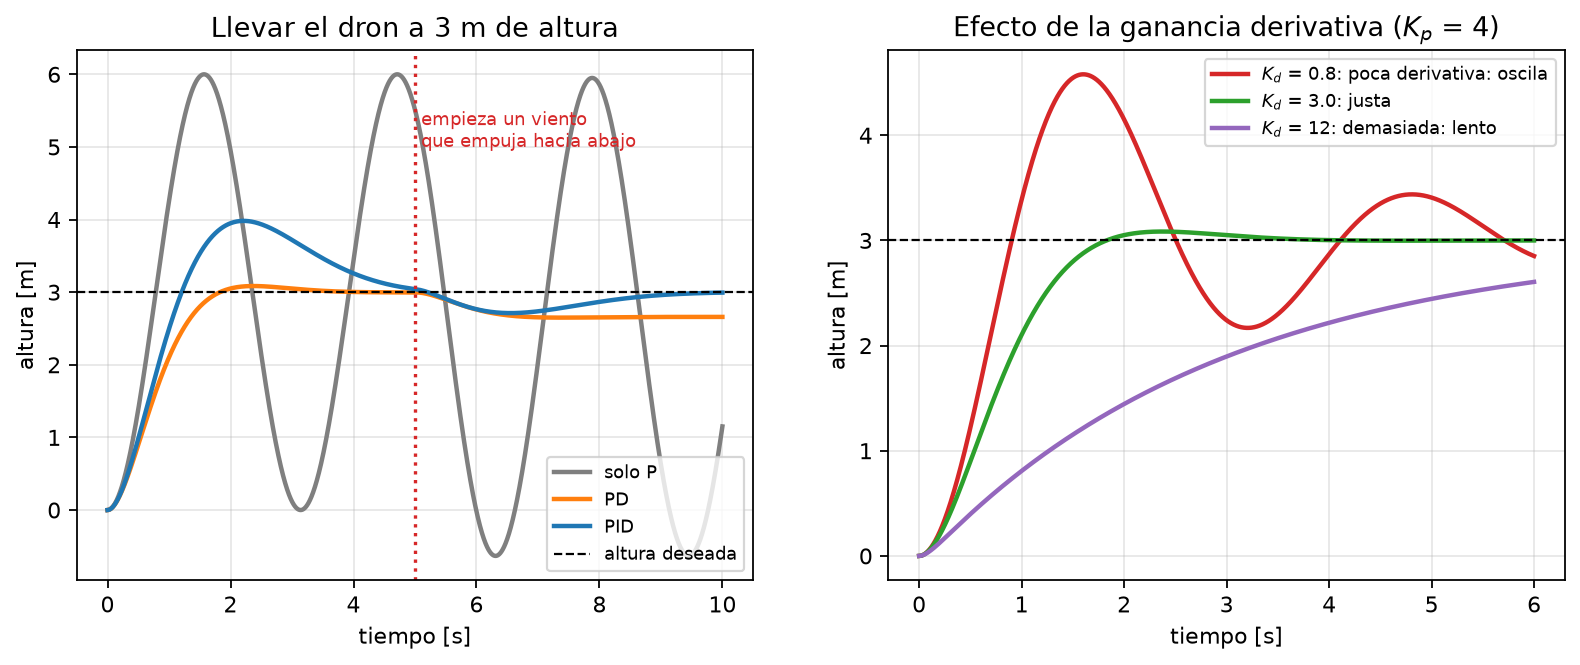
\includegraphics[width=\textwidth]{c_pid.png}
\caption{Simulación de la altura de una masa de 2.2~kg (como el Tarot). Izquierda: solo P oscila; PD
llega pero el viento (desde $t=5$~s) le deja un error; PID lo corrige. Derecha: efecto de $K_d$.}
\label{fig:pid}
\end{figure}

\begin{recuerda}
\textbf{P} empuja hacia el objetivo, \textbf{D} frena para no pasarse, \textbf{I} corrige lo que
queda. El PID es, de lejos, el controlador más usado en el mundo, incluidos los drones comerciales.
\end{recuerda}

\section{Cómo se lee una respuesta}

Para comparar controladores se les pide un cambio brusco de referencia (un \textbf{escalón}) y se
mide:

\begin{figure}[H]
\centering
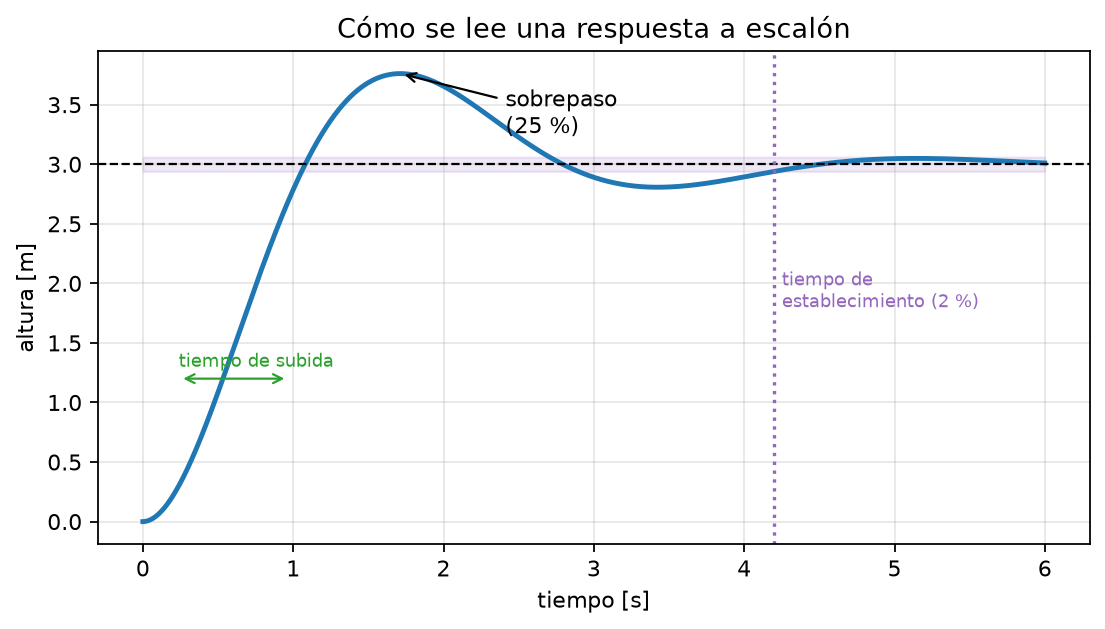
\includegraphics[width=0.8\textwidth]{c_respuesta.png}
\caption{Medidas típicas de una respuesta a escalón.}
\end{figure}

\begin{description}
  \item[Sobrepaso:] cuánto se pasa del objetivo.
  \item[Tiempo de subida:] cuánto tarda en ir del 10~\% al 90~\% del cambio.
  \item[Tiempo de establecimiento:] a partir de cuándo se queda cerca del objetivo (por ejemplo, a
        menos del 2~\%).
  \item[Error en estado estacionario:] lo que queda de error cuando todo se calma.
\end{description}
En este proyecto se usa sobre todo el \textbf{error RMS} (raíz del promedio de los errores al cuadrado)
durante una órbita con viento: un solo número que resume qué tan bien sigue el dron su trayectoria.

\section{Control en cascada: así se controla un dron}

El dron no puede ``moverse a la derecha'' directamente: tiene que inclinarse. Por eso hay dos lazos,
uno dentro del otro:

\begin{figure}[H]
\centering
\begin{tikzpicture}[blq/.style={draw,rounded corners,fill=#1,minimum width=2.6cm,minimum height=1cm,align=center,font=\small},blq/.default=white,
  fl/.style={-{Stealth[length=2.2mm]},thick}]
  \node (ref) at (-0.6,0) {\small posición deseada};
  \node[blq=blue!10] (pos) at (2.6,0) {lazo de posición\\(lento: PD o STA)};
  \node[blq=red!10] (act) at (6.4,0) {lazo de actitud\\(rápido: PD en SO(3))};
  \node[blq=black!5] (mix) at (10,0) {mezclador};
  \node[blq=orange!15] (dron) at (10,-2.2) {dron};
  \draw[fl] (ref) -- (pos);
  \draw[fl] (pos) -- node[above,font=\scriptsize,align=center]{empuje e\\inclinación} (act);
  \draw[fl] (act) -- node[above,font=\scriptsize]{pares} (mix);
  \draw[fl] (mix) -- node[right,font=\scriptsize]{4 velocidades} (dron);
  \draw[fl] (dron.west) -- ++(-3,0) -| node[pos=0.75,right,font=\scriptsize]{orientación} (act.south);
  \draw[fl] (dron.west) -- ++(-6.8,0) -| node[pos=0.75,right,font=\scriptsize]{posición} (pos.south);
\end{tikzpicture}
\caption{Control en cascada del cuadrirrotor.}
\label{fig:cascada}
\end{figure}

\begin{enumerate}
  \item El \textbf{lazo de posición} compara dónde está el dron con dónde debe estar y calcula qué
        fuerza total necesita: cuánto empuje y hacia dónde apuntarlo.
  \item Apuntar el empuje significa inclinar el dron: el \textbf{lazo de actitud} calcula los pares
        para alcanzar esa inclinación. Es mucho más rápido que el de posición.
  \item El \textbf{mezclador} convierte empuje y pares en la velocidad de cada motor.
\end{enumerate}
En este proyecto, el lazo interno es siempre el mismo y lo que se cambia es el externo: el PD
(línea base) o el super-twisting adaptativo, que es el tema del próximo capítulo.

\begin{ejercicio}
Compara el PD con el STA en la órbita con viento:
\begin{lstlisting}[style=bash]
ros2 launch cuadrirotor_sim simulacion.launch.py vehiculo:=tarot650 mundo:=bosque controlador:=pd mision:=orbita viento:=true csv:=$HOME/pd.csv
ros2 launch cuadrirotor_sim simulacion.launch.py vehiculo:=tarot650 mundo:=bosque controlador:=sta mision:=orbita viento:=true csv:=$HOME/sta.csv
python3 ~/ros2_ws/src/cuadrirotor_sim/scripts/metricas.py ~/pd.csv ~/sta.csv
\end{lstlisting}
\end{ejercicio}

\chapter{Modos deslizantes y super-twisting}

\begin{enpocas}
Qué es una superficie deslizante, por qué el control por modos deslizantes resiste perturbaciones
que no conoce, qué es el \emph{chattering}, cómo lo resuelve el super-twisting y por qué conviene que
su ganancia se adapte sola.
\end{enpocas}

\section{El problema: perturbaciones que no conocemos}

El PID funciona bien, pero sus ganancias se ajustan para un caso. Si el viento cambia mucho, o el dron
lleva una carga distinta, rinde peor. El \textbf{control por modos deslizantes} (SMC, \emph{sliding
mode control}) nace con otra idea: no importa cuál sea la perturbación, siempre que no pase de cierto
tamaño, el controlador la vence.

\section{La superficie deslizante}

Se define una variable que combina el error y su velocidad:
\begin{equation}
s = \dot e + \lambda e ,\qquad \lambda > 0 .
\end{equation}
Si logramos que $s = 0$, entonces $\dot e = -\lambda e$: el error decae exponencialmente a cero solo,
como $e(t) = e_0\,e^{-\lambda t}$. La recta $s = 0$ en el plano (error, velocidad del error) es la
\textbf{superficie deslizante}. El trabajo se divide en dos:
\begin{enumerate}
  \item \textbf{llegar} a la superficie, aunque haya perturbación;
  \item \textbf{quedarse} en ella y ``deslizarse'' hasta el origen.
\end{enumerate}

\begin{figure}[H]
\centering
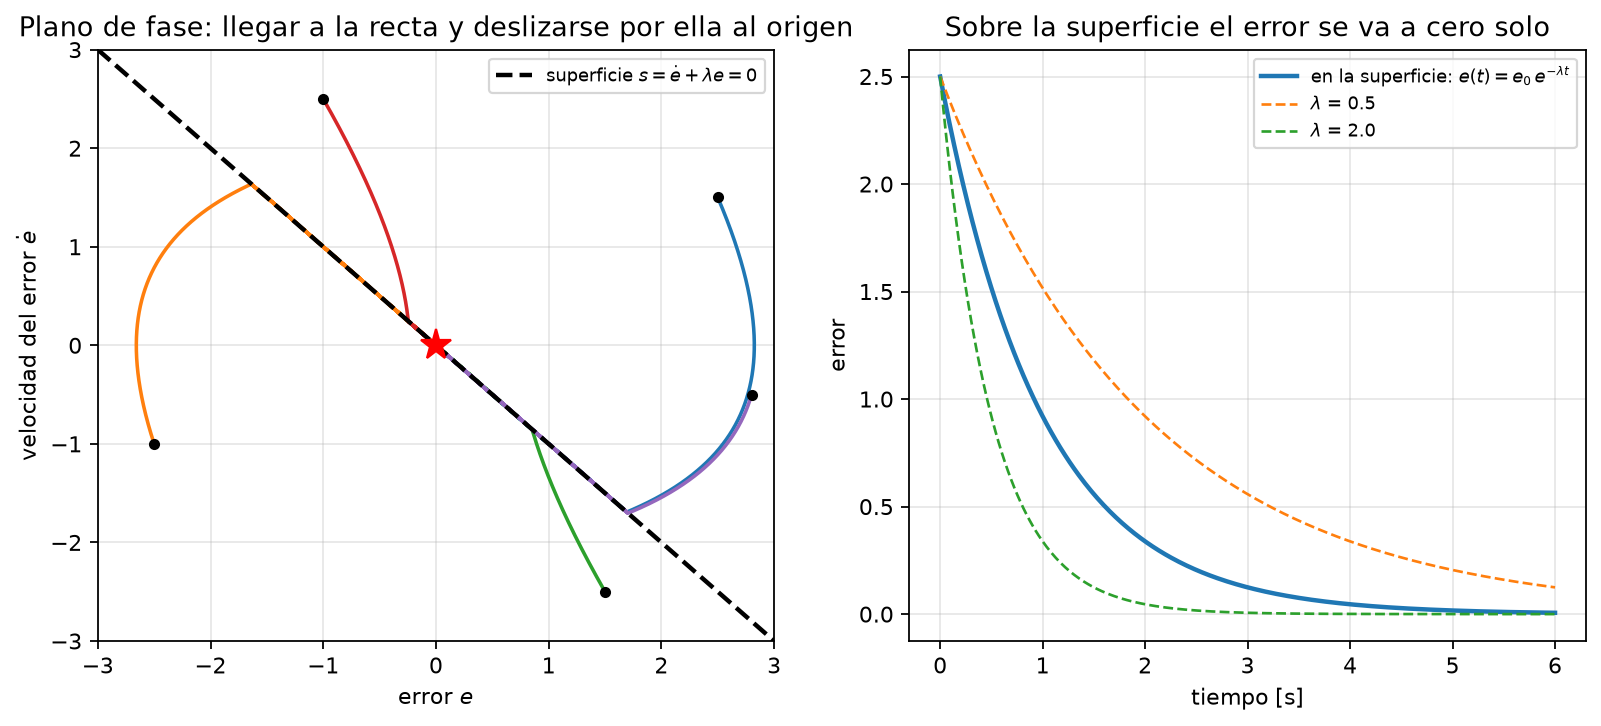
\includegraphics[width=\textwidth]{c_deslizante.png}
\caption{Izquierda: desde cualquier punto, el estado viaja hasta la recta $s=0$ y luego se desliza
por ella hasta el origen (error cero). Derecha: sobre la superficie, $\lambda$ decide qué tan rápido
se va el error.}
\label{fig:deslizante}
\end{figure}

\begin{ejemplo}
Imagina una canica en un tobogán con forma de ``V''. Caiga donde caiga, rueda hasta el fondo de la
``V'' (llegar a la superficie) y luego baja por el fondo del canal hasta la meta (deslizarse). El
viento puede empujarla, pero si las paredes son lo bastante empinadas, no la saca del canal.
\end{ejemplo}

\section{El control clásico: empujar con todo}

El SMC más simple empuja siempre con la misma fuerza hacia la superficie:
\begin{equation}
u = -k\,\sgn(s) ,
\end{equation}
donde $\sgn(s)$ vale $+1$ si $s>0$ y $-1$ si $s<0$. Si $k$ es mayor que la perturbación más grande,
el estado siempre llega a la superficie. Es muy robusto, pero tiene un problema grave.

\section{El chattering}

Al llegar a $s=0$, el control salta de $+k$ a $-k$ una y otra vez, muy rápido. Eso es el
\textbf{chattering} (``castañeteo''): vibraciones que desgastan los motores, gastan batería y pueden
excitar dinámicas que el modelo no considera.

\begin{figure}[H]
\centering
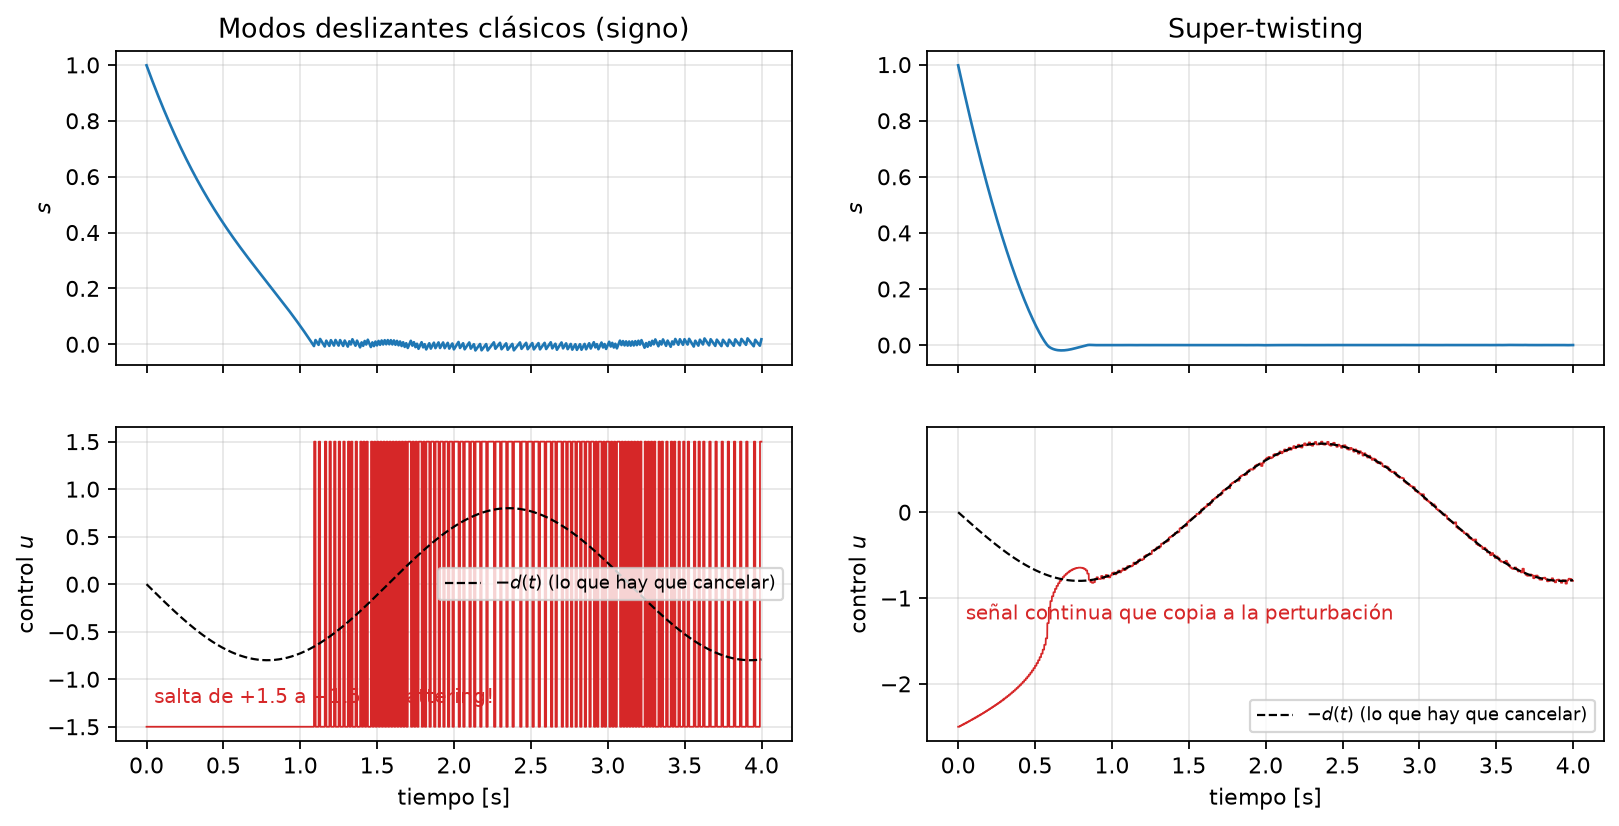
\includegraphics[width=\textwidth]{c_chattering.png}
\caption{Izquierda: el SMC clásico lleva $s$ a cero, pero su control salta sin parar entre $+1.5$ y
$-1.5$. Derecha: el super-twisting también lleva $s$ a cero, con una señal de control suave que copia
a la perturbación para cancelarla.}
\label{fig:chattering}
\end{figure}

\section{Super-twisting: robusto y suave}

El algoritmo \textbf{super-twisting} (STA) es un modo deslizante ``de segundo orden'' que esconde la
parte discontinua detrás de una integral:
\begin{align}
u &= -k_1 |s|^{1/2}\sgn(s) + \nu,\\
\dot\nu &= -k_2\,\sgn(s).
\end{align}
\begin{itemize}
  \item El primer término empuja hacia la superficie con una fuerza que se hace pequeña cerca de ella
        (por la raíz cuadrada).
  \item El segundo, $\nu$, es la integral de un signo: va creciendo o decreciendo poco a poco hasta
        igualar a la perturbación. Como una integral es continua, \textbf{el control $u$ es continuo}.
\end{itemize}
El resultado: $s$ y $\dot s$ llegan a cero en tiempo finito, aunque haya una perturbación que cambie
(con derivada acotada), y sin chattering en el control continuo (figura~\ref{fig:chattering},
derecha).

\begin{recuerda}
El super-twisting tiene la robustez de los modos deslizantes pero entrega una señal de control
continua. Necesita dos ganancias, $k_1$ y $k_2$, lo bastante grandes para la perturbación.
\end{recuerda}

\section{Ganancia adaptativa: no exagerar}

¿Qué tan grandes deben ser $k_1$ y $k_2$? Si son pequeñas, una ráfaga fuerte gana; si son grandes,
el control es agresivo todo el tiempo y amplifica el ruido. La versión \textbf{adaptativa} (Shtessel,
Taleb y Plestan, 2012) las ajusta sola:
\begin{equation}
\dot k_1 = \begin{cases} +w_1\sqrt{\gamma_1/2} & \text{si } |s| > \mu \ \text{(vamos mal: subir)}\\
                          -w_1\sqrt{\gamma_1/2} & \text{si } |s| < \mu \ \text{(vamos bien: bajar)}\end{cases}
\qquad k_2 = 2\varepsilon k_1 .
\end{equation}
$\mu$ es una pequeña tolerancia: si $s$ se mantiene dentro de $\pm\mu$, la ganancia baja; si se sale,
sube.

\begin{figure}[H]
\centering
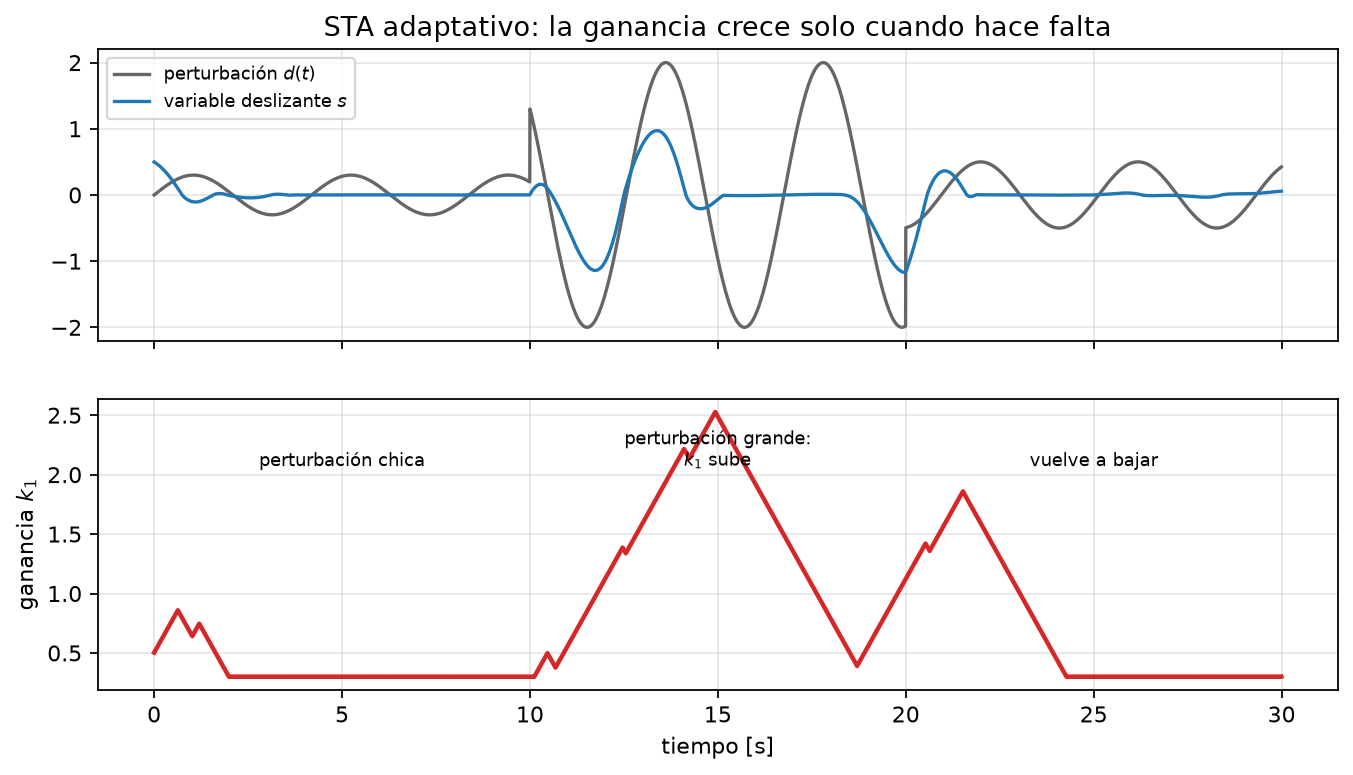
\includegraphics[width=0.85\textwidth]{c_adaptativo.png}
\caption{La perturbación crece de $t=10$ a 20~s: la ganancia $k_1$ sube para vencerla y luego vuelve a
bajar.}
\end{figure}

\begin{aviso}
Elegir $\mu$ es delicado. En el dron, el retardo de los motores y del lazo de actitud produce una
pequeña oscilación de $s$ que nunca desaparece (un \emph{ciclo límite}). Si $\mu$ es menor que esa
oscilación, la ganancia crece sin parar y el dron se vuelve inestable. Por eso en la simulación $\mu$
es distinto para cada eje y cada vehículo (0.3~m/s en $x$, $y$ y 0.03~m/s en $z$ para el Tarot).
\end{aviso}

\section{Cómo se usa en el dron}

Por cada eje ($x$, $y$, $z$) del lazo de posición:
\begin{equation}
s = e_v + \lambda e_p ,\qquad a = a_d + \lambda e_v - u ,
\end{equation}
donde $e_p$ y $e_v$ son los errores de posición y velocidad y $a_d$ la aceleración que pide la
trayectoria. Con esa elección resulta $\dot s = u + d$: exactamente el sistema para el que está
diseñado el super-twisting, con $d$ la perturbación (viento y todo lo que el modelo no sabe). Los
detalles están en el capítulo~\ref{cap:control-sim}.

\chapter{Del papel a la computadora: discretización}

\begin{enpocas}
Por qué una computadora no puede aplicar una ecuación ``continua'', qué es el periodo de muestreo,
la diferencia entre discretizar de forma explícita e implícita, y por qué esto es el corazón del
proyecto.
\end{enpocas}

\section{La computadora ve a saltos}

Las ecuaciones del capítulo anterior son \emph{continuas}: dicen qué hacer en cada instante. Una
computadora, en cambio, trabaja a pasos: lee los sensores, calcula y manda la orden a los motores, y
repite cada $T_s$ segundos (el \textbf{periodo de muestreo}; en la simulación, 5~ms por omisión, es
decir 200 veces por segundo). Entre una orden y la siguiente, el motor recibe la misma (eso se llama
\textbf{retenedor de orden cero}).

\begin{figure}[H]
\centering
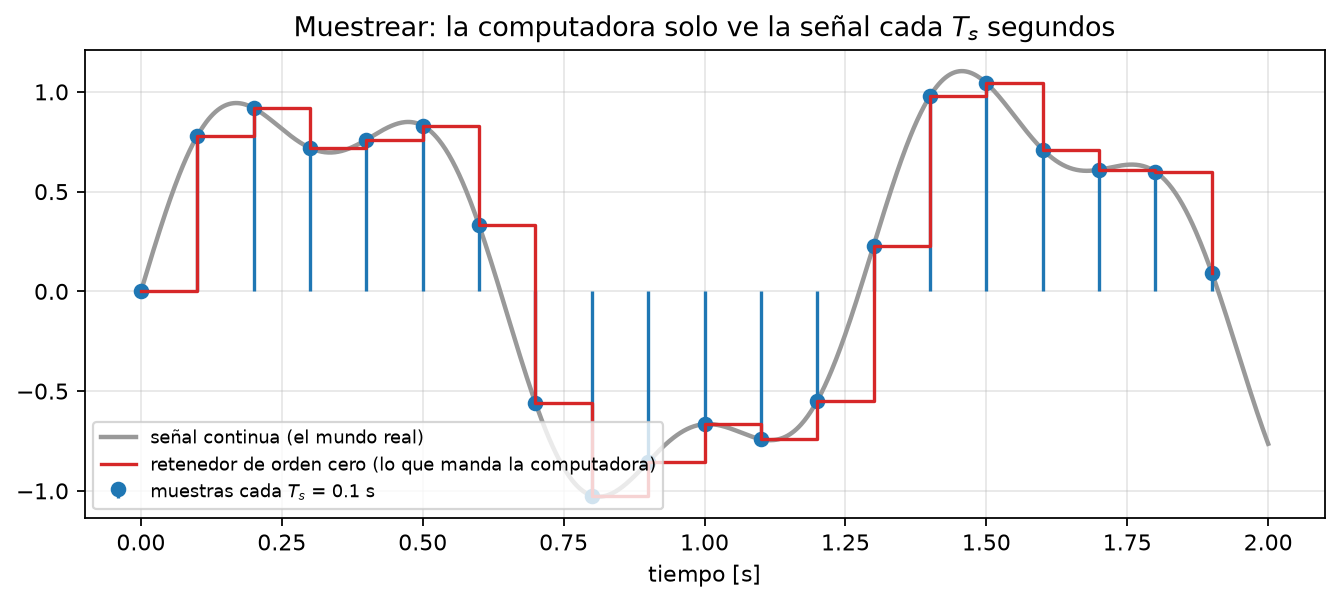
\includegraphics[width=0.9\textwidth]{c_muestreo.png}
\caption{La computadora solo ``ve'' la señal en los instantes de muestreo y mantiene su orden constante
entre ellos.}
\end{figure}

\textbf{Discretizar} es convertir una ley de control continua en una receta de pasos
$k = 0, 1, 2, \dots$ Hay muchas formas de hacerlo y no todas se portan igual.

\section{Un ejemplo para entender: explícito contra implícito}

Tomemos la ecuación más simple que se va a cero: $\dot x = -a x$ (por ejemplo, una taza de café que se
enfría). Con paso $T_s$:

\begin{description}
  \item[Euler explícito] (usar el valor de \emph{ahora}):
        $x_{k+1} = x_k - T_s a\,x_k = (1 - aT_s)\,x_k$.
  \item[Euler implícito] (usar el valor \emph{que va a tener}):
        $x_{k+1} = x_k - T_s a\,x_{k+1} \;\Rightarrow\; x_{k+1} = \dfrac{x_k}{1 + aT_s}$.
\end{description}

Si el paso es pequeño, los dos dan casi lo mismo. Pero si $aT_s > 2$, el explícito multiplica por un
número de valor absoluto mayor que 1 en cada paso: \textbf{explota}, aunque la ecuación original sea
perfectamente estable. El implícito divide siempre por algo mayor que 1: \textbf{nunca explota}.

\begin{figure}[H]
\centering
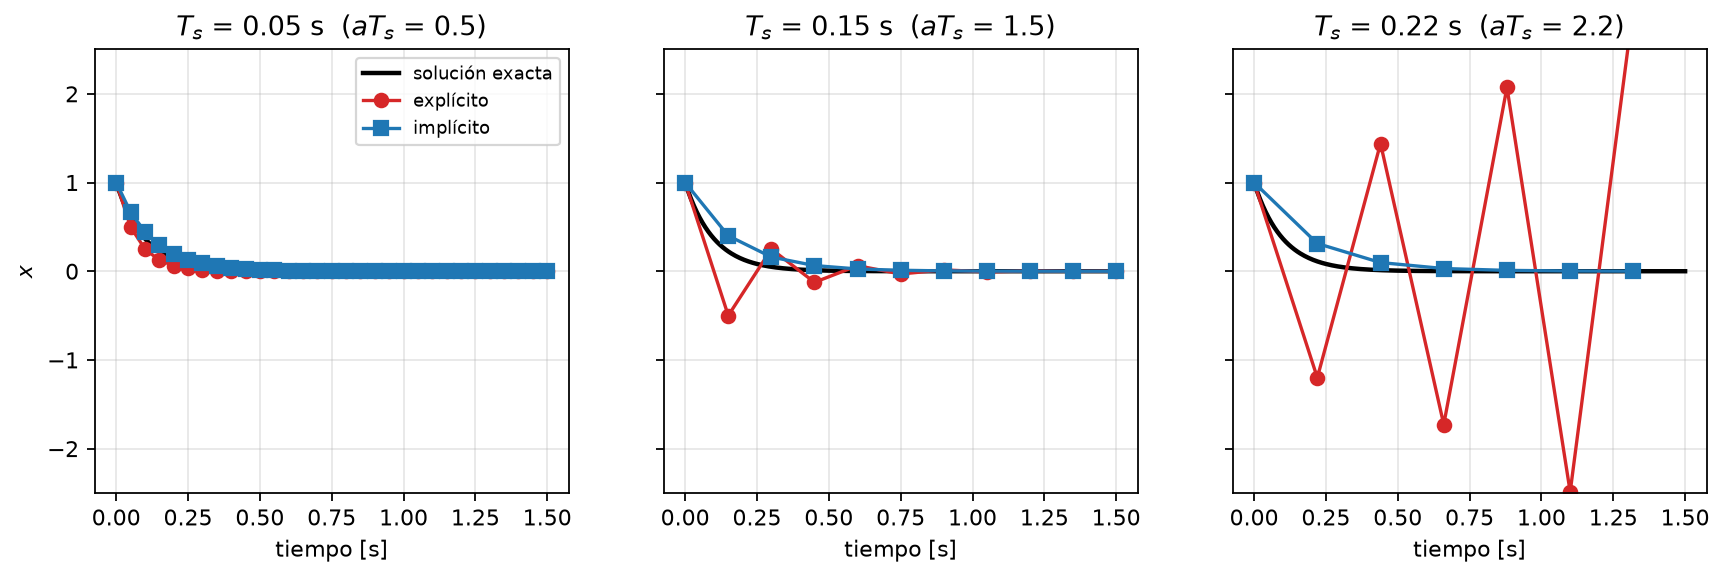
\includegraphics[width=\textwidth]{c_euler.png}
\caption{La misma ecuación $\dot x = -ax$ con $a = 10$, resuelta con pasos cada vez mayores. El
implícito siempre se va a cero; el explícito oscila y, con $aT_s > 2$, diverge.}
\label{fig:euler}
\end{figure}

\begin{recuerda}
\textbf{Explícito}: calculo el siguiente paso con lo que sé ahora; es simple pero puede pasarse.
\textbf{Implícito}: planteo una ecuación con el valor futuro y la resuelvo; cuesta un poco más pero
respeta mejor el comportamiento del sistema continuo.
\end{recuerda}

\section{El problema con los modos deslizantes}

Con la función signo pasa algo parecido, y peor. En la versión explícita del super-twisting:
\begin{equation}
u_k = -k_1|s_k|^{1/2}\sgn(s_k) + \nu_k,\qquad \nu_{k+1} = \nu_k - T_s k_2\sgn(s_k).
\end{equation}
Cerca de $s = 0$, el signo cambia en cada paso y $s$ queda ``rebotando'' alrededor de cero con una
amplitud que crece con la ganancia: es el \textbf{chattering numérico}, producido por la
discretización y no por la física. Y como el STA adaptativo \emph{sube} la ganancia cuando $s$ no está
quieto, el chattering puede alimentar a la adaptación.

\section{La discretización implícita del super-twisting}

La idea (Brogliato, Polyakov y Efimov, 2020) es preguntar: ``¿qué control lleva a $s$ a donde
debería estar en el siguiente paso?'' Se plantea una ecuación con el valor futuro $\tilde s$:
\begin{equation}
\tilde s + T_s k_1|\tilde s|^{1/2}\xi + T_s^2 k_2\,\xi = s_k + T_s\nu_k,\qquad \xi\in\Sgn(\tilde s),
\end{equation}
donde $\Sgn$ es el signo ``como conjunto'': en $\tilde s = 0$ puede valer cualquier número entre $-1$
y $1$. Esa libertad es la clave: si el estado está cerca de la superficie, la ecuación tiene la
solución $\tilde s = 0$ exactamente, con $\xi$ intermedio, en lugar de saltar de $+1$ a $-1$. La
solución se obtiene con una fórmula cerrada (sección~\ref{sec:discretizaciones}).

\begin{figure}[H]
\centering
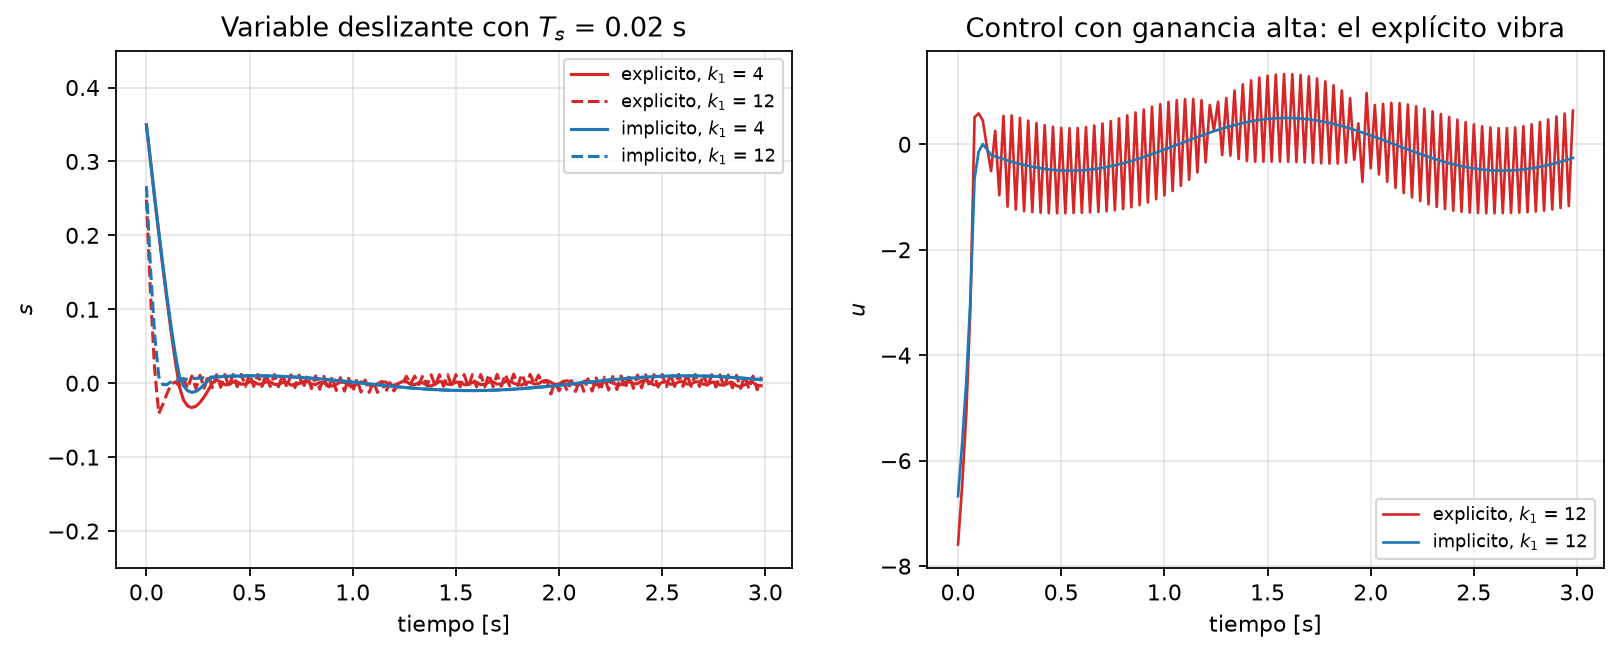
\includegraphics[width=\textwidth]{c_discreto.png}
\caption{Super-twisting con $T_s = 20$~ms y una perturbación senoidal. Con la ganancia alta
($k_1 = 12$), el explícito vibra; el implícito da la misma señal suave que con la ganancia baja.}
\label{fig:discreto}
\end{figure}

\begin{recuerda}
La hipótesis del proyecto: con la discretización implícita, el super-twisting adaptativo conserva su
robustez y elimina el chattering numérico, y deja de ser sensible a que la ganancia sea demasiado
grande. La simulación permite comprobarlo (y ya mostró matices, sección~\ref{sec:observaciones}).
\end{recuerda}

\section{Tres versiones en el código}

\cod{sta.py} implementa las tres, y se elige al lanzar con \cod{esquema:=}:
\begin{description}
  \item[\cod{explicito}] la de arriba;
  \item[\cod{semi_implicito}] el signo se evalúa en el paso siguiente pero la raíz $|s|^{1/2}$ en el
        actual (más fácil de resolver);
  \item[\cod{implicito}] la ecuación completa.
\end{description}

\begin{ejercicio}
Corre la órbita con viento con los tres esquemas y un periodo de muestreo grande, y compara la banda
de $s$ con \cod{metricas.py}:
\begin{lstlisting}[style=bash]
src/cuadrirotor_sim/scripts/corrida.sh ~/corridas/exp.csv 50 esquema=explicito Ts=0.02 k1_0=4.0 adaptativo=false
src/cuadrirotor_sim/scripts/corrida.sh ~/corridas/imp.csv 50 esquema=implicito Ts=0.02 k1_0=4.0 adaptativo=false
src/cuadrirotor_sim/scripts/metricas.py ~/corridas/*.csv
\end{lstlisting}
\end{ejercicio}

\chapter{El control del dron en la simulación}
\label{cap:control-sim}

\begin{enpocas}
Cómo quedaron implementados, en la simulación, el PD en cascada y el super-twisting adaptativo con sus
tres discretizaciones, con qué parámetros, y qué resultados dieron con el Tarot y con viento.
\end{enpocas}

\section{Modelo}

Cuerpo rígido con posición $p\in\mathbb{R}^3$ (marco del mundo), orientación $R\in SO(3)$ y
velocidad angular $\omega$ (marco del cuerpo):
\begin{equation}
m\ddot p = -mg\,e_3 + T R e_3 + d(t),\qquad
J\dot\omega = -\omega\times J\omega + \tau,\qquad \dot R = R\,\hat\omega,
\end{equation}
con $T$ y $\tau$ producidos por los motores a través del mezclador y $d(t)$ la perturbación
(viento). Gazebo integra el modelo completo (incluidos el retardo de los motores, el arrastre de
los rotores y el contacto con el suelo); el controlador usa los mismos $m$, $J$, $k_f$ y $k_m$.

\section{Controlador PD en cascada (línea base)}

\cod{controlador_pd.py} corre cada $T_s$ (5~ms por omisión) de tiempo simulado y manda las
velocidades de rotor con retenedor de orden cero.

\textbf{Lazo externo.} Con $e_p = p_d - p$ y $e_v = v_d - v$:
\begin{equation}
F = m\,(a + g\,e_3),\qquad a = a_d + K_p e_p + K_d e_v,\qquad T = F\cdot R e_3,
\end{equation}
con $K_p = \operatorname{diag}(4,4,6)$ y $K_d = \operatorname{diag}(3,3,4)$.

\textbf{Actitud deseada.} A partir de la dirección de $F$ y la guiñada deseada $\psi_d$:
\begin{equation}
b_3 = \frac{F}{\|F\|},\quad b_{1c} = (\cos\psi_d,\sin\psi_d,0),\quad
b_2 = \frac{b_3\times b_{1c}}{\|b_3\times b_{1c}\|},\quad R_d = [\,b_2\times b_3,\ b_2,\ b_3\,].
\end{equation}

\textbf{Lazo interno} (PD sobre SO(3)):
\begin{equation}
e_R = \tfrac12\big(R_d^\top R - R^\top R_d\big)^\vee,\qquad
\tau = -K_R e_R - K_\omega\,\omega + \omega\times J\omega .
\end{equation}

\section{Super-twisting adaptativo (STA)}

\cod{controlador_sta.py} reemplaza la aceleración del lazo externo. Por eje:
\begin{equation}
s = e_v + \lambda e_p,\qquad a = a_d + \lambda e_v - u
\quad\Rightarrow\quad \dot s = u + d(t),
\end{equation}
y $u$ es el super-twisting con ganancia adaptativa (Shtessel, Taleb y Plestan, 2012):
\begin{align}
u &= -k_1 |s|^{1/2}\sgn(s) + \nu, & \dot\nu &= -k_2\sgn(s),\\
\dot k_1 &= \begin{cases} w_1\sqrt{\gamma_1/2}\;\sgn(|s|-\mu) & k_1 > k_{1,min}\\ \eta & \text{en otro caso}\end{cases},
& k_2 &= 2\varepsilon k_1 .
\end{align}

\subsection{Discretizaciones}
\label{sec:discretizaciones}

Con periodo $T_s$ y $a_k = s_k + T_s\nu_k$, \cod{sta.py} implementa:

\begin{description}
  \item[Explícita] $u_k = -k_1|s_k|^{1/2}\sgn(s_k) + \nu_k$,\quad $\nu_{k+1} = \nu_k - T_s k_2\sgn(s_k)$.
  \item[Semi-implícita] el término discontinuo se evalúa en el paso siguiente y $|s|^{1/2}$ en el actual:
        $\tilde s + (T_s k_1|s_k|^{1/2} + T_s^2 k_2)\,\xi = a_k$, con $\xi\in\Sgn(\tilde s)$.
  \item[Implícita] (Brogliato, Polyakov y Efimov, 2020):
  \begin{equation}
  \tilde s + T_s k_1|\tilde s|^{1/2}\xi + T_s^2 k_2\,\xi = a_k,\qquad \xi\in\Sgn(\tilde s),
  \end{equation}
  cuya solución única es
  \begin{equation}
  \begin{cases}
  \tilde s = 0,\quad \xi = a_k/(T_s^2k_2) & \text{si } |a_k|\le T_s^2k_2,\\[2pt]
  \tilde s = \sgn(a_k)\,w^2,\quad w = \dfrac{-T_sk_1+\sqrt{T_s^2k_1^2+4(|a_k|-T_s^2k_2)}}{2} & \text{en otro caso.}
  \end{cases}
  \end{equation}
\end{description}
En los dos esquemas implícitos $\tilde s$ es la predicción nominal de $s_{k+1}$, $\nu_{k+1} = \nu_k
- T_s k_2\xi$ y $u_k = (\tilde s - s_k)/T_s$. El código de la solución implícita:

\begin{lstlisting}[style=py]
@staticmethod
def resolver_implicito(a, b, c):
    """Solución única de  x + b |x|^(1/2) xi + c xi = a,  xi en Sgn(x),  b, c > 0."""
    abs_a = np.abs(a)
    dentro = abs_a <= c
    w = (-b + np.sqrt(b**2 + 4.0 * np.maximum(abs_a - c, 0.0))) / 2.0
    x = np.where(dentro, 0.0, np.sign(a) * w**2)
    xi = np.where(dentro, a / np.where(dentro, c, 1.0), np.sign(a))
    return x, xi
\end{lstlisting}

\subsection{Parámetros}

En \cod{config/parametros.yaml}, sección \cod{controlador_sta}: $\lambda = (1.5, 1.5, 2.0)$,
$k_{1,0} = 1$, $\varepsilon = 1$, $w_1 = 2$, $\gamma_1 = 1$, $k_{1,min} = 0.5$, $\eta = 0.1$. Los que
dependen del vehículo van en su YAML: para el Tarot $\mu = (0.3, 0.3, 0.03)$ y $k_{1,max} = 3$.
El esquema se elige al lanzar:
\begin{lstlisting}[style=bash]
ros2 launch cuadrirotor_sim simulacion.launch.py vehiculo:=tarot650 mundo:=bosque \
    controlador:=sta esquema:=implicito mision:=orbita viento:=true csv:=$HOME/corrida.csv
\end{lstlisting}

\section{Resultados}

La misión \cod{orbita} despega a 3~m, se traslada y describe una órbita de radio 4~m alrededor del
foco $(8,5)$ con la cámara apuntando a él, con viento desde
$t = 15$~s. Las métricas las calcula \cod{scripts/metricas.py}.

\begin{figure}[H]
\centering
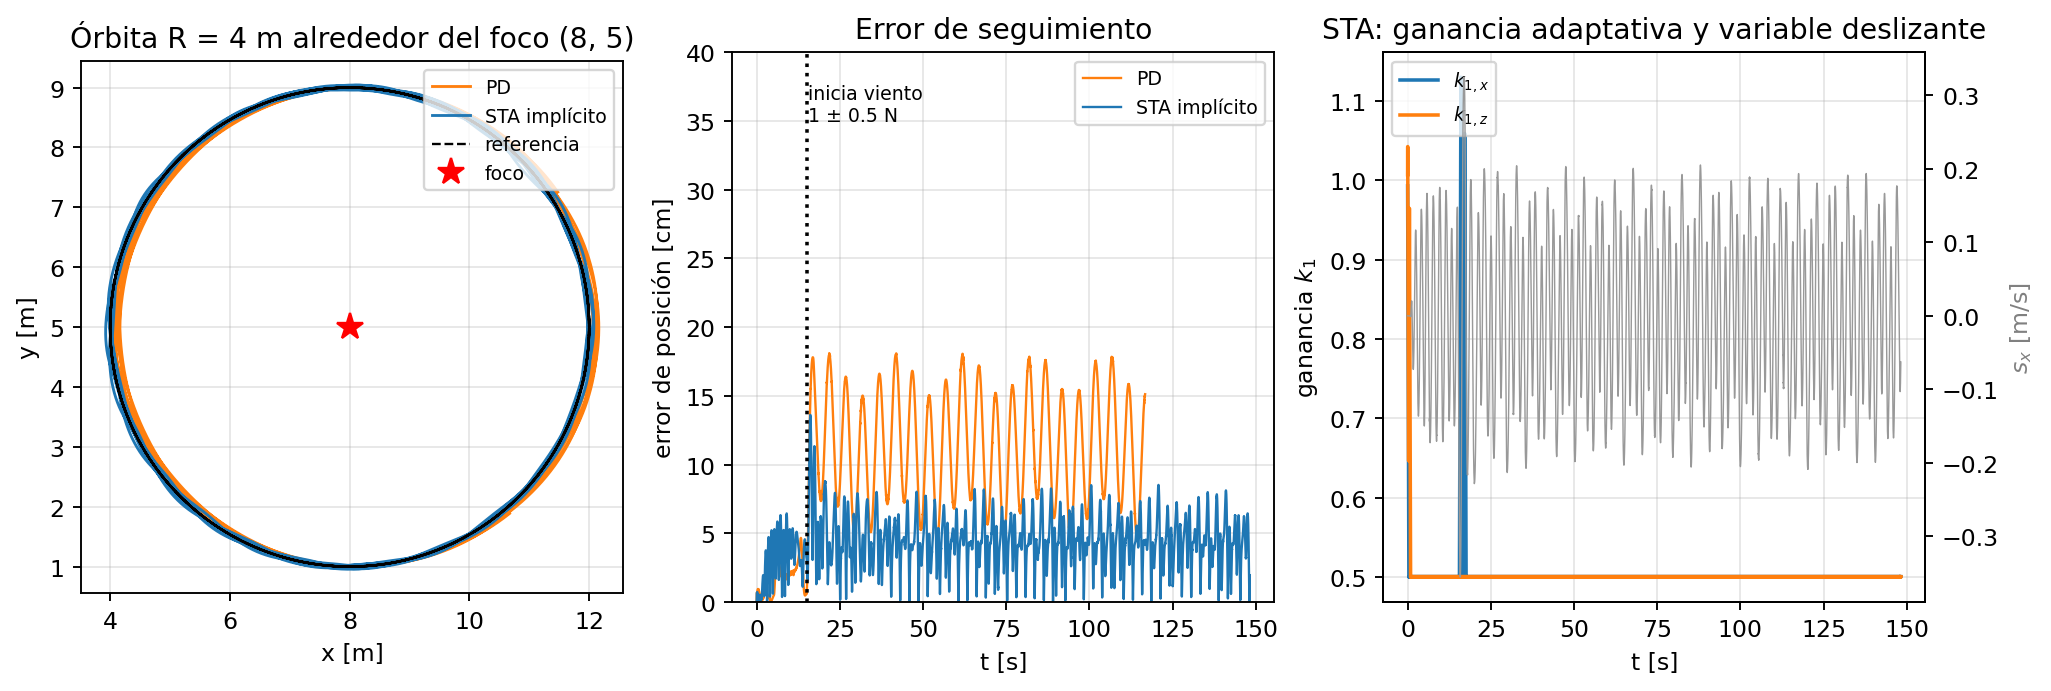
\includegraphics[width=\textwidth]{orbita_pd_sta.png}
\caption{Tarot 650 en el mundo \cod{bosque}, órbita con viento de $1\pm0.5$~N (corridas del 23 de
octubre). El STA implícito reduce el error RMS con viento de 11.9~cm (PD) a 4.8~cm. La ganancia
$k_1$ baja hasta $k_{1,min}$: el umbral $\mu$ del Tarot queda por encima del ciclo límite.}
\label{fig:orbita}
\end{figure}

\begin{table}[H]
\centering\small
\begin{tabular}{llccc}
\toprule
\textbf{Vehículo} & \textbf{Controlador} & \textbf{RMS sin viento} & \textbf{RMS con viento} & \textbf{Máx. con viento} \\ \midrule
cuadrirrotor & PD en cascada & --- & 17.7 cm & 28.5 cm \\
cuadrirrotor & STA explícito & --- & 2.4 cm & 4.7 cm \\
cuadrirrotor & STA semi-implícito & --- & 2.1 cm & 4.0 cm \\
cuadrirrotor & STA implícito & --- & 2.1 cm & 4.3 cm \\
Tarot 650 & PD en cascada & 2.8 cm & 11.9 cm & 18.1 cm \\
Tarot 650 & STA implícito & 3.3 cm & 4.8 cm & 8.5 cm \\
Tarot 650 & ArduCopter 4.7.2 & --- & 13.7 cm & --- \\
\bottomrule
\end{tabular}
\caption{Error de seguimiento en la órbita ($T_s = 5$~ms). Las filas del cuadrirrotor y la de
ArduPilot son del 21--22 de octubre; las del Tarot con PD y STA, de las corridas de la
figura~\ref{fig:orbita}.}
\end{table}

\subsection{Observaciones}
\label{sec:observaciones}

\begin{enumerate}
  \item Con perturbación, el esquema implícito de las ec.~(9)--(12) deja una banda
        $|s|\approx T_s|d|$, \textbf{independiente de la ganancia} (insensible a la
        sobreestimación), pero no proporcional a $T_s^2k_2$ como plantea la hipótesis: la predicción
        nominal supone $d=0$. Con \cod{estimar_perturbacion: true} (estimación $\hat d$ del paso
        anterior; Acary, Brogliato y Orlov, 2012) la banda baja a $\approx T_s^2\max|\dot d|$.
  \item En $x$, $y$ el retardo del lazo de actitud y de los motores induce un ciclo límite
        ($|s|\approx$ 0.05--0.1~m/s en el cuadrirrotor, 0.2--0.35~m/s en el Tarot). Si $\mu$ queda
        por debajo de él, la ganancia crece sin control y el lazo se inestabiliza; por eso $\mu$
        es por eje y por vehículo.
  \item La velocidad que publica Gazebo es un promedio de 10 muestras ($\approx$4.5~ms de retraso
        a 1~kHz): forma parte de la dinámica no modelada.
\end{enumerate}

\section{Agregar un controlador}

Se hereda de \cod{ControladorPD}, se sobrescribe \cod{aceleracion(ep, ev, ad)} y se registra el
ejecutable en \cod{setup.py}. Así quedó el STA:
\begin{lstlisting}[style=py]
def aceleracion(self, ep, ev, ad):
    self.s = ev + self.lam * ep
    return ad + self.lam * ev - self.sta(self.s)
\end{lstlisting}


\part{Ver el mundo: visión computacional}
\chapter{Qué es una imagen para una computadora}
\label{cap:imagen}

\begin{enpocas}
Píxeles y canales de color, cómo forma una imagen una cámara (modelo estenopeico), qué es el campo de
visión, qué ve la cámara del dron y cómo se pasa de un píxel a un punto del mundo.
\end{enpocas}

\section{Una imagen es una tabla de números}

Para nosotros una foto es una escena; para la computadora es una \textbf{tabla de números}. La cámara
del dron entrega imágenes de 640 columnas por 480 filas: 307\,200 \textbf{píxeles} (de \emph{picture
element}). Cada píxel tiene tres números entre 0 y 255: cuánto rojo, cuánto verde y cuánto azul (RGB).
$(0,0,0)$ es negro, $(255,255,255)$ blanco y $(230,140,55)$ un naranja de fuego.

\begin{figure}[H]
\centering
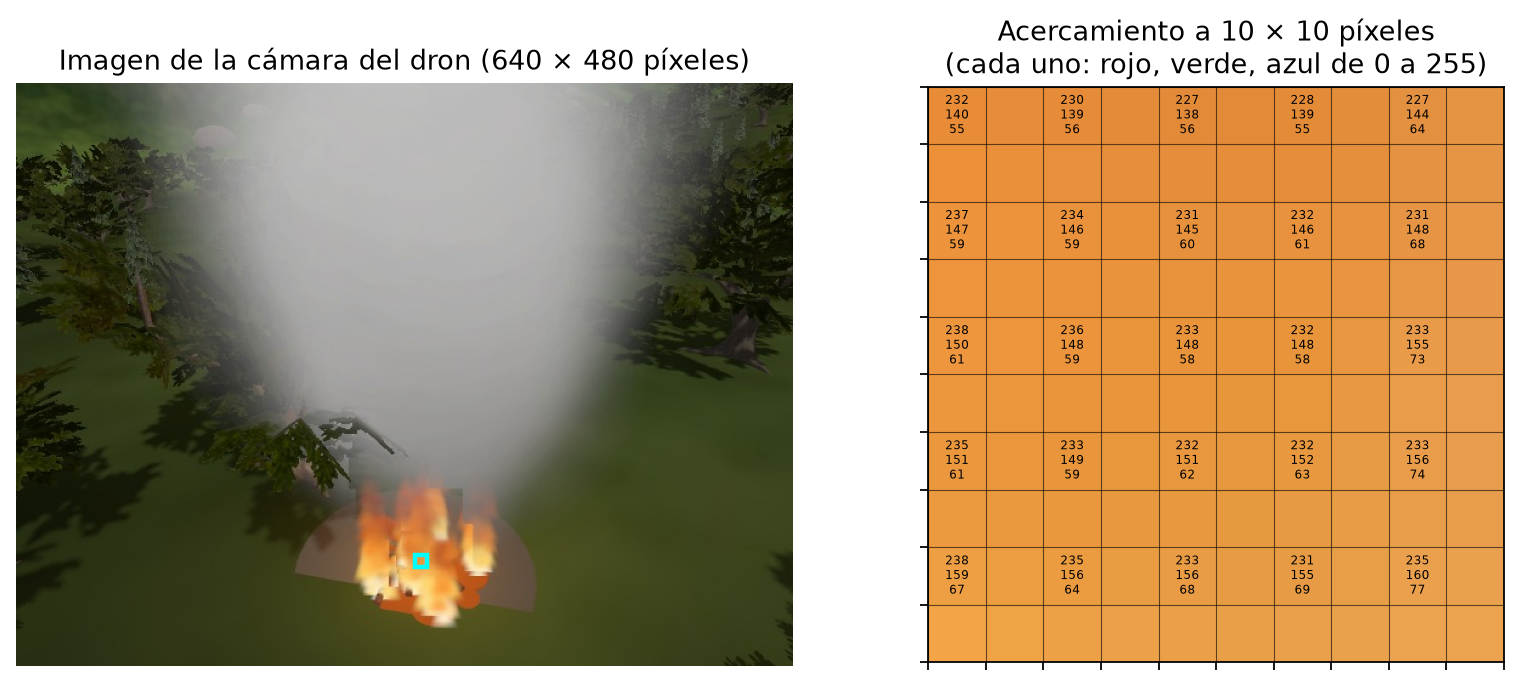
\includegraphics[width=\textwidth]{c_pixeles.png}
\caption{Una imagen de la cámara del dron y un acercamiento a 10$\times$10 píxeles de las llamas:
mucho rojo (230), algo de verde (145) y poco azul (60).}
\label{fig:pixeles}
\end{figure}

Las tres tablas (rojo, verde, azul) se llaman \textbf{canales}. Verlas por separado ayuda a entender
por qué el fuego es fácil de distinguir: brilla mucho en el canal rojo y poco en el azul, mientras que
el humo es claro en los tres.

\begin{figure}[H]
\centering
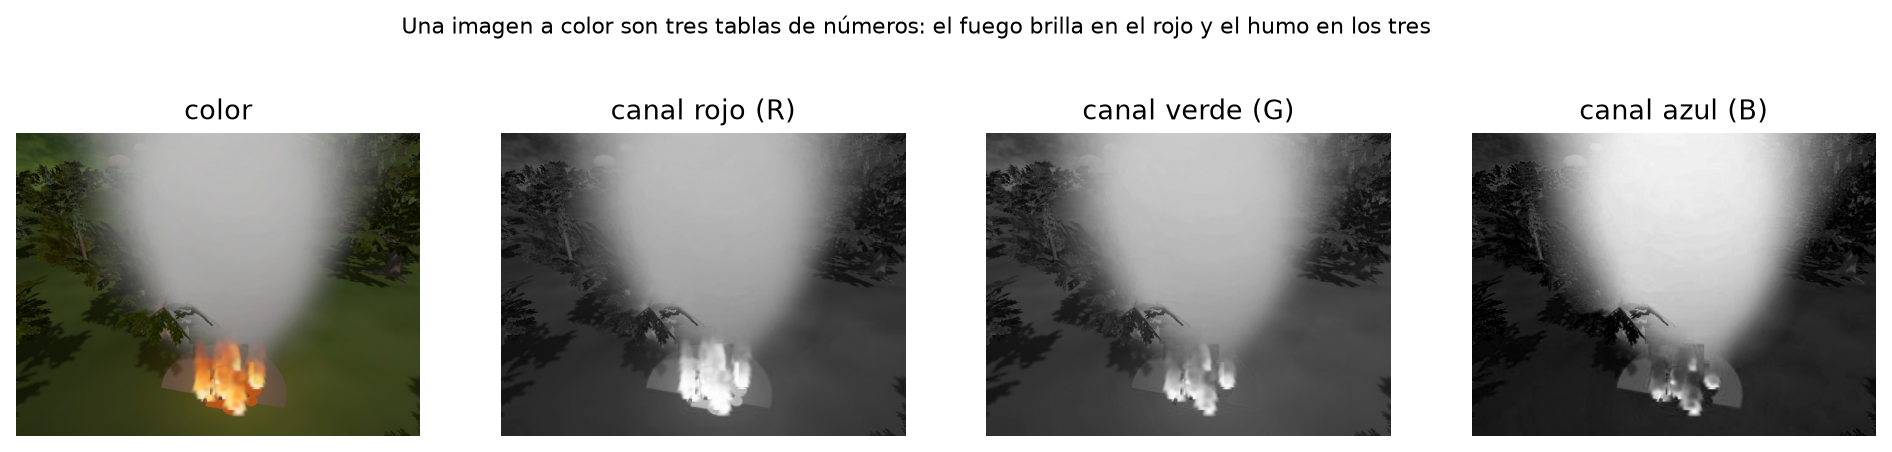
\includegraphics[width=\textwidth]{c_rgb.png}
\caption{La misma imagen separada en sus tres canales (más claro = valor más alto).}
\end{figure}

\begin{ejemplo}
Una imagen es como una hoja de cálculo gigante donde cada celda está pintada de un color. Un programa
de visión ``lee'' esa hoja buscando patrones de números, igual que tú buscarías un patrón de colores.
\end{ejemplo}

Un video son imágenes una tras otra: la cámara simulada entrega 15 por segundo en el tópico
\cod{/cuadrirotor/camara}.

\section{Cómo forma una imagen una cámara}

El modelo más útil es el de la \textbf{cámara estenopeica} (\emph{pinhole}): una caja oscura con un
agujerito. La luz de cada punto del mundo entra en línea recta por el agujero y llega a un punto del
sensor. Por semejanza de triángulos, un punto a distancia $Z$ y desplazado $X$ del eje aparece en la
imagen a
\begin{equation}
u = f\,\frac{X}{Z},
\end{equation}
donde $f$ es la \textbf{distancia focal} (en píxeles). Los objetos lejanos se ven más pequeños:
dividir entre $Z$ es la \emph{perspectiva}.

\begin{figure}[H]
\centering
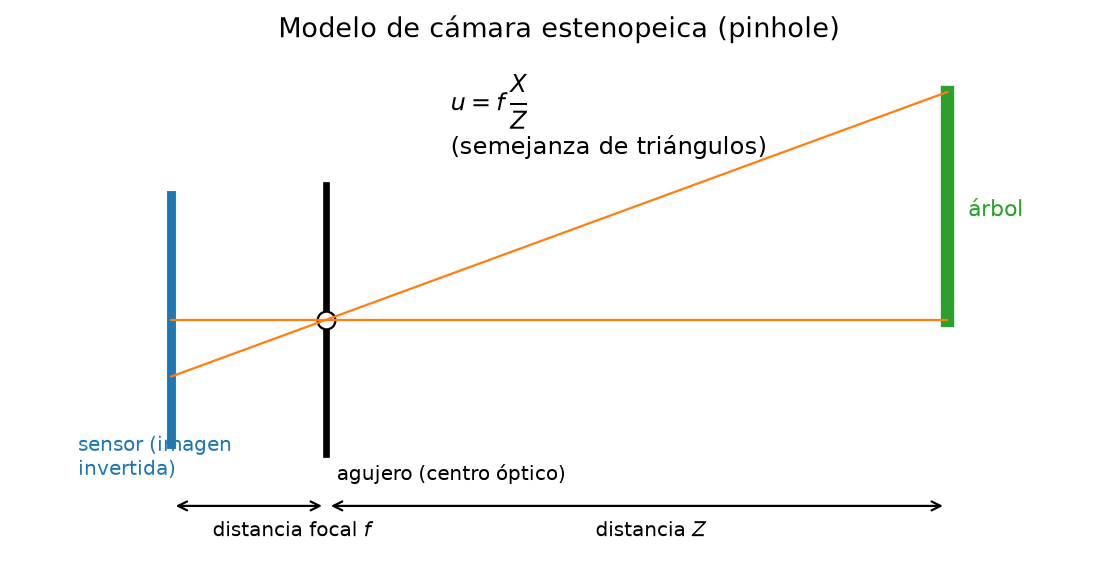
\includegraphics[width=0.85\textwidth]{c_estenopeica.png}
\caption{El modelo estenopeico: la imagen se forma por rayos rectos que pasan por el centro óptico.}
\end{figure}

\section{Campo de visión}

El \textbf{campo de visión} (FOV) es qué tan ancho ve la cámara. La del dron tiene un campo horizontal
de 1.3~rad (74°); con una imagen de 640 píxeles de ancho eso da
\begin{equation}
f = \frac{640/2}{\tan(1.3/2)} \approx 418\ \text{píxeles}.
\end{equation}
Va inclinada 30° hacia abajo: así ve el horizonte (para descubrir humo lejos) y también el suelo
delante del dron.

\begin{figure}[H]
\centering
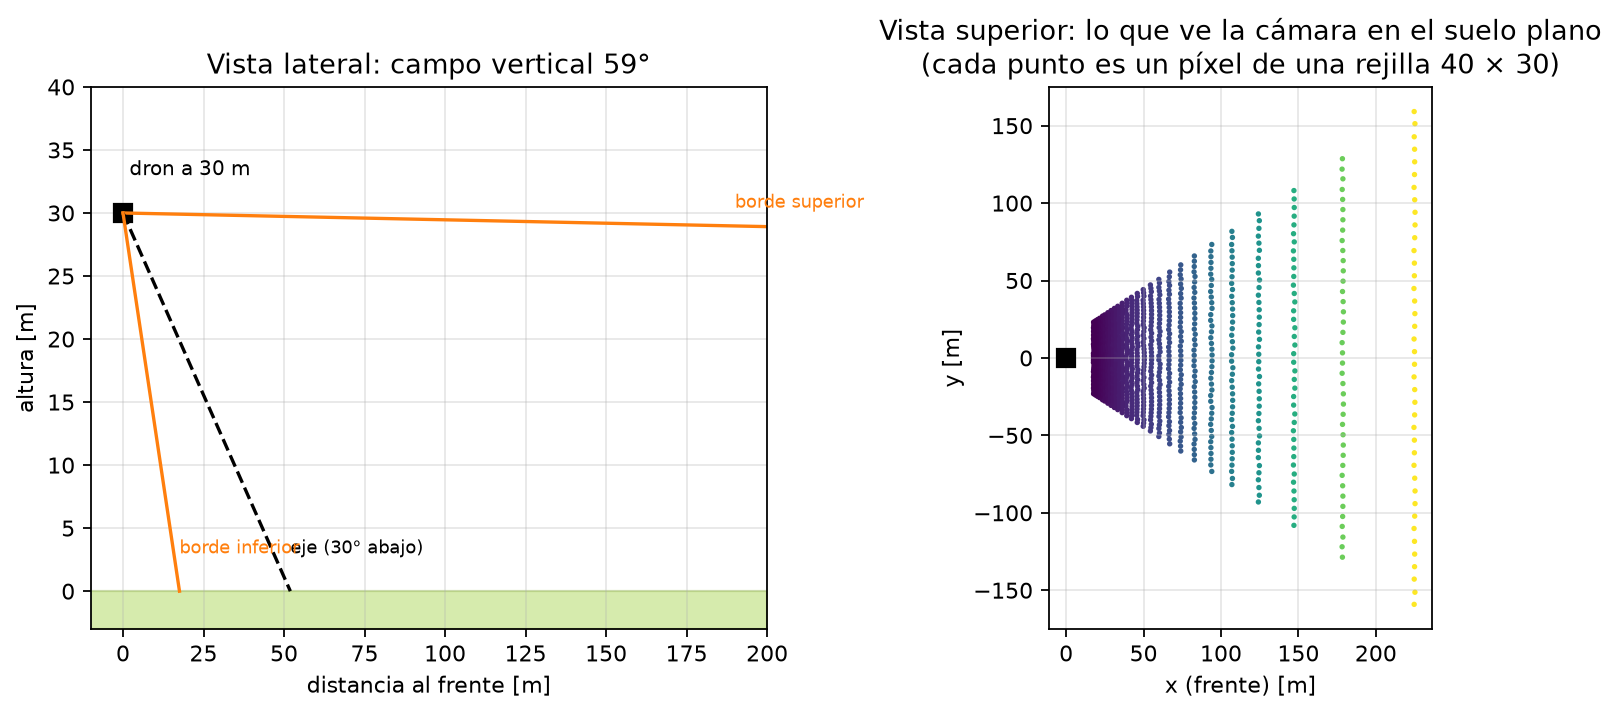
\includegraphics[width=\textwidth]{c_fov.png}
\caption{Qué ve la cámara desde 30~m de altura. Izquierda: el borde superior de la imagen casi toca
el horizonte y el inferior cae a 18~m del dron. Derecha: la ``huella'' de la imagen en el suelo; los
píxeles de arriba cubren mucho más terreno que los de abajo.}
\label{fig:fov}
\end{figure}

\begin{figure}[H]
\centering
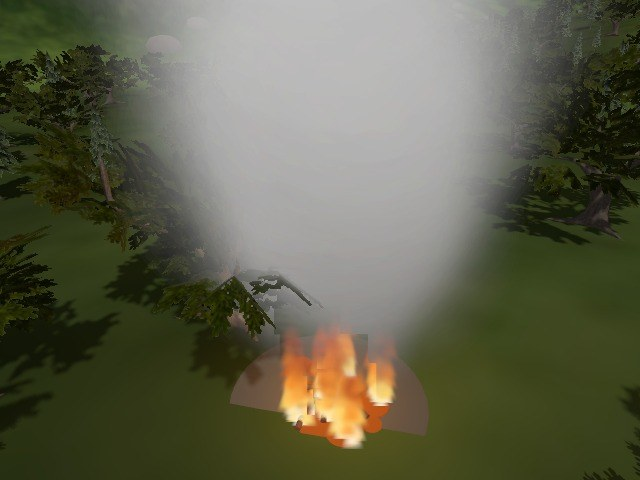
\includegraphics[width=0.32\textwidth]{ds_fuego_humo.jpg}\hfill
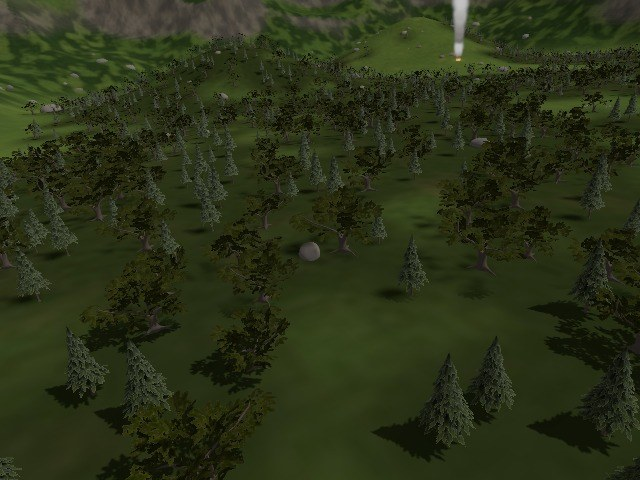
\includegraphics[width=0.32\textwidth]{ds_humo_lejano.jpg}\hfill
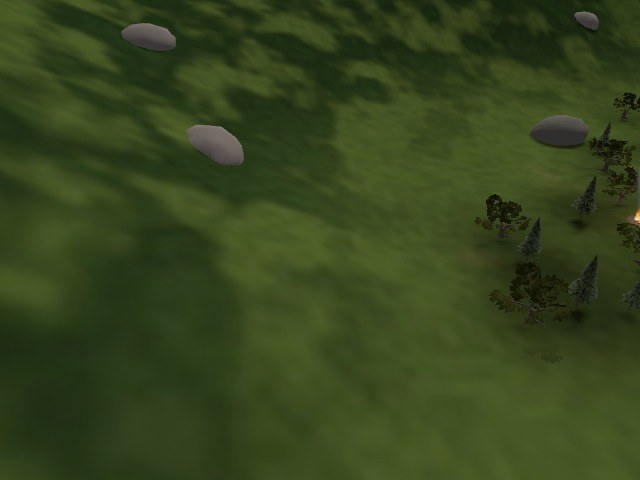
\includegraphics[width=0.32\textwidth]{ds_sin_fuego.jpg}
\caption{Imágenes de la cámara del dron simulado: fuego y humo de cerca, humo a lo lejos (la columna
blanca arriba a la derecha) y una escena sin fuego con rocas.}
\end{figure}

\section{Del píxel al mundo: rayos}

La cámara pierde una dimensión: un píxel no dice a qué distancia está lo que muestra, solo en qué
\emph{dirección}. Cada píxel corresponde a un \textbf{rayo} que sale de la cámara. Invirtiendo el
modelo estenopeico, el rayo del píxel $(u,v)$ en el marco de la cámara es
\begin{equation}
d_{cam} = \Big(1,\ -\frac{u - W/2}{f},\ -\frac{v - H/2}{f}\Big),
\end{equation}
y se pasa al mundo con la orientación del dron y de la cámara. Para saber \emph{dónde} está lo que se
ve, hace falta otra información:
\begin{itemize}
  \item un modelo del terreno: el punto está donde el rayo toca el suelo (así se estima el fuego,
        capítulo~\ref{cap:conceptos-autonomia});
  \item o varias vistas desde lugares distintos: donde se cruzan los rayos (triangulación, como se
        hace con el humo).
\end{itemize}

\begin{recuerda}
Una cámara da direcciones, no distancias. Para ubicar algo en el mapa hay que cruzar su rayo con el
terreno o con otros rayos.
\end{recuerda}

\chapter{Redes neuronales y YOLO sin complicaciones}

\begin{enpocas}
Qué es aprender a partir de ejemplos, cómo funciona una neurona artificial, qué hace una convolución,
cómo detecta objetos YOLO, cómo se entrena (datos, etiquetas, épocas, pérdida) y cómo se mide qué tan
bien funciona (IoU, precisión, recall, mAP).
\end{enpocas}

\section{Programar contra aprender}

¿Cómo le explicarías a una computadora qué es el humo? Podrías intentar reglas: ``muchos píxeles
grises claros juntos''. Pero las nubes también lo son, y el humo a contraluz es oscuro. Las reglas
escritas a mano fallan pronto. El \textbf{aprendizaje automático} hace lo contrario: se le dan miles de
ejemplos con la respuesta correcta (``aquí hay humo, en este rectángulo'') y el programa ajusta sus
propios parámetros hasta acertar. Eso es \textbf{entrenar}.

\section{La neurona artificial}

\begin{figure}[H]
\centering
\begin{tikzpicture}[
  n/.style={circle,draw,fill=#1,minimum size=0.8cm,inner sep=0},n/.default=blue!12,
  fl/.style={-{Stealth[length=2mm]}}]
  \foreach \i/\t in {1/$x_1$,2/$x_2$,3/$x_3$} { \node (x\i) at (0,-\i*1.1) {\t}; }
  \node[n=orange!20,minimum size=1.3cm] (s) at (3,-2.2) {$\sum$};
  \node[draw,rounded corners,fill=green!12] (f) at (5.2,-2.2) {activación};
  \node (y) at (7.3,-2.2) {salida};
  \foreach \i/\w in {1/$w_1$,2/$w_2$,3/$w_3$} { \draw[fl] (x\i) -- node[above,font=\scriptsize]{\w} (s); }
  \node (b) at (3,-0.4) {$b$ (sesgo)}; \draw[fl] (b) -- (s);
  \draw[fl] (s) -- (f); \draw[fl] (f) -- (y);
  % red
  \begin{scope}[xshift=9.5cm,yshift=-0.4cm]
    \foreach \i in {1,...,4} \node[n] (a\i) at (0,-\i*0.9) {};
    \foreach \i in {1,...,5} \node[n=orange!20] (b\i) at (1.8,-\i*0.9+0.45) {};
    \foreach \i in {1,...,3} \node[n=green!15] (c\i) at (3.6,-\i*0.9-0.45) {};
    \foreach \i in {1,...,4} \foreach \j in {1,...,5} \draw[black!35] (a\i) -- (b\j);
    \foreach \i in {1,...,5} \foreach \j in {1,...,3} \draw[black!35] (b\i) -- (c\j);
    \node[font=\scriptsize] at (0,-4.4) {entrada}; \node[font=\scriptsize] at (1.8,-4.4) {capa oculta}; \node[font=\scriptsize] at (3.6,-4.4) {salida};
  \end{scope}
\end{tikzpicture}
\caption{Izquierda: una neurona multiplica cada entrada por un \emph{peso}, suma todo y pasa el
resultado por una función de activación. Derecha: una red son muchas neuronas en capas.}
\end{figure}

Una neurona artificial hace una cuenta muy simple:
\begin{equation}
\text{salida} = \text{activación}\big(w_1x_1 + w_2x_2 + \dots + w_nx_n + b\big).
\end{equation}
Los \textbf{pesos} $w_i$ dicen qué tan importante es cada entrada. Sola, una neurona es poca cosa;
millones de ellas en capas pueden reconocer caras, voces o fuego. Entrenar es buscar los pesos que
hacen que la red acierte. YOLO26n tiene unos 2.5 millones de pesos.

\section{Convoluciones: buscar patrones locales}

Conectar cada píxel con cada neurona sería enorme. Las redes para imágenes usan
\textbf{convoluciones}: un filtro pequeño (por ejemplo $3\times3$ números) que se desliza por toda la
imagen; en cada posición multiplica sus números por los píxeles de abajo y suma. Según los números del
filtro, resalta bordes, manchas, texturas...

\begin{figure}[H]
\centering
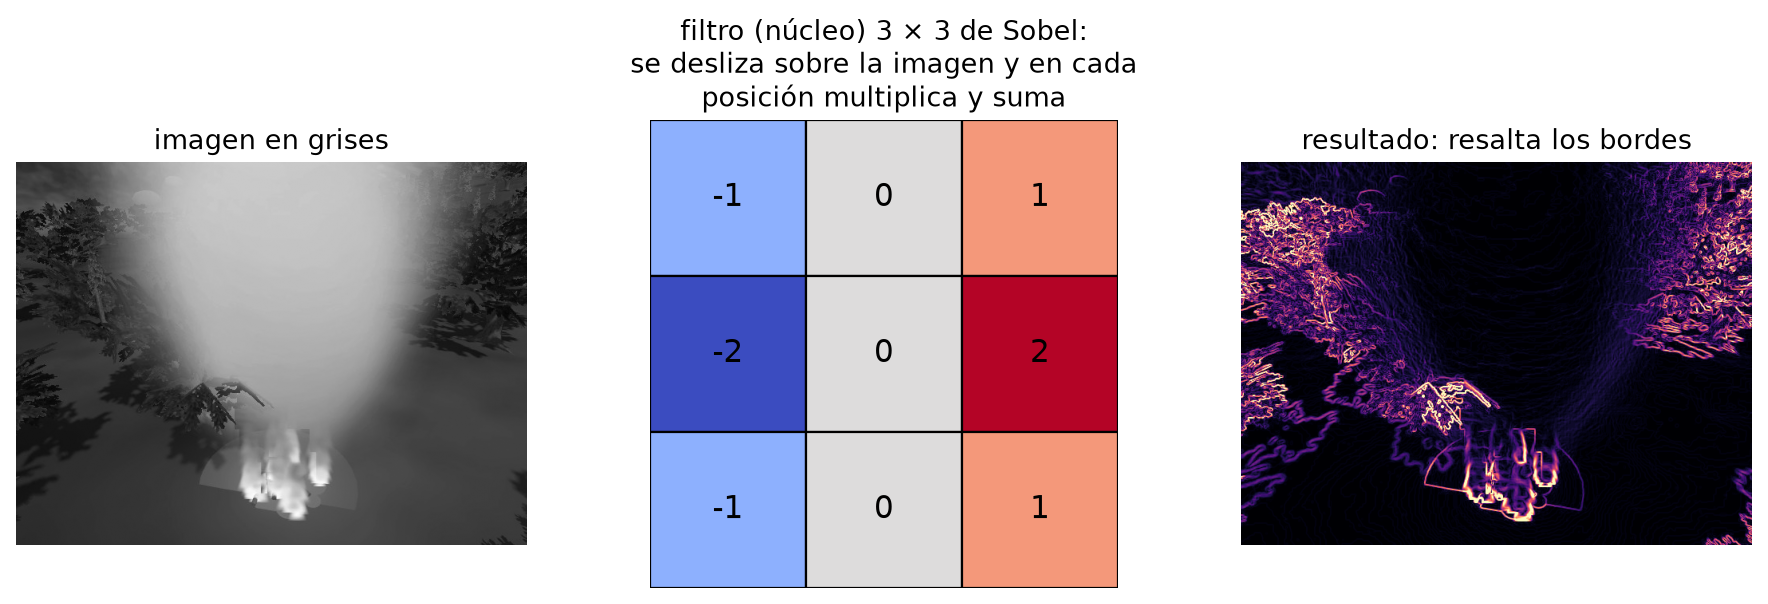
\includegraphics[width=\textwidth]{c_convolucion.png}
\caption{Un filtro de bordes (Sobel) aplicado a la imagen del incendio. En una red convolucional los
números de los filtros no se eligen a mano: se aprenden.}
\end{figure}

Una \textbf{red convolucional} (CNN) apila muchas capas de filtros: las primeras detectan bordes y
colores, las intermedias texturas (llamas, humo, hojas) y las últimas objetos completos.

\section{Detectar objetos: cajas y clases}

Hay varias tareas de visión: \emph{clasificar} (¿hay fuego en la imagen?), \emph{detectar} (¿dónde?)
y \emph{segmentar} (¿qué píxeles exactamente?). Necesitamos \textbf{detección}: el dron debe saber en
qué parte de la imagen está el fuego para calcular hacia dónde está. Un detector entrega una lista de
\textbf{cajas} (rectángulos), cada una con una \textbf{clase} (``fuego'' o ``humo'') y una
\textbf{confianza} entre 0 y 1.

\section{YOLO}

\textbf{YOLO} (\emph{You Only Look Once}, ``solo miras una vez'') es una familia de detectores muy
rápida: en lugar de revisar la imagen por pedazos, una sola pasada de la red predice todas las cajas a
la vez. Por eso sirve en tiempo real, incluso en un dron. Usamos \textbf{YOLO26n}, la versión más
reciente de Ultralytics en su tamaño más pequeño (\emph{nano}); en la GPU procesa una imagen en pocos
milisegundos.

\begin{figure}[H]
\centering
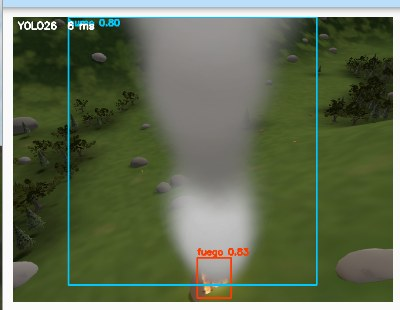
\includegraphics[width=0.55\textwidth]{yolo_panel.jpg}
\caption{Lo que entrega YOLO: cajas con su clase y su confianza (``fuego 0.83'').}
\end{figure}

\section{Entrenar: datos, etiquetas y épocas}

\begin{description}
  \item[Dataset:] el conjunto de imágenes de ejemplo. Se usaron 6000 imágenes del simulador.
  \item[Etiquetas:] para cada imagen, las cajas correctas. En formato YOLO, un archivo de texto con
        una línea por objeto: clase y caja (centro, ancho y alto, como fracción de la imagen).
  \item[Entrenamiento y validación:] el dataset se parte en dos. La red aprende con uno
        (\emph{entrenamiento}) y se evalúa con el otro, que nunca ve al aprender (\emph{validación}).
        Así se mide si generaliza o solo memoriza.
  \item[Época:] una pasada completa por todas las imágenes de entrenamiento. Se hicieron 60.
  \item[Pérdida (loss):] un número que mide qué tan mal predice la red. Entrenar es bajarla, ajustando
        los pesos un poquito en la dirección que la reduce (\emph{descenso de gradiente}).
  \item[Ajuste fino (fine-tuning):] no se empezó de cero, sino de una red ya entrenada con el dataset
        COCO (80 clases de objetos comunes). La red ya sabe ``ver'' y solo aprende las clases nuevas.
\end{description}

\begin{figure}[H]
\centering
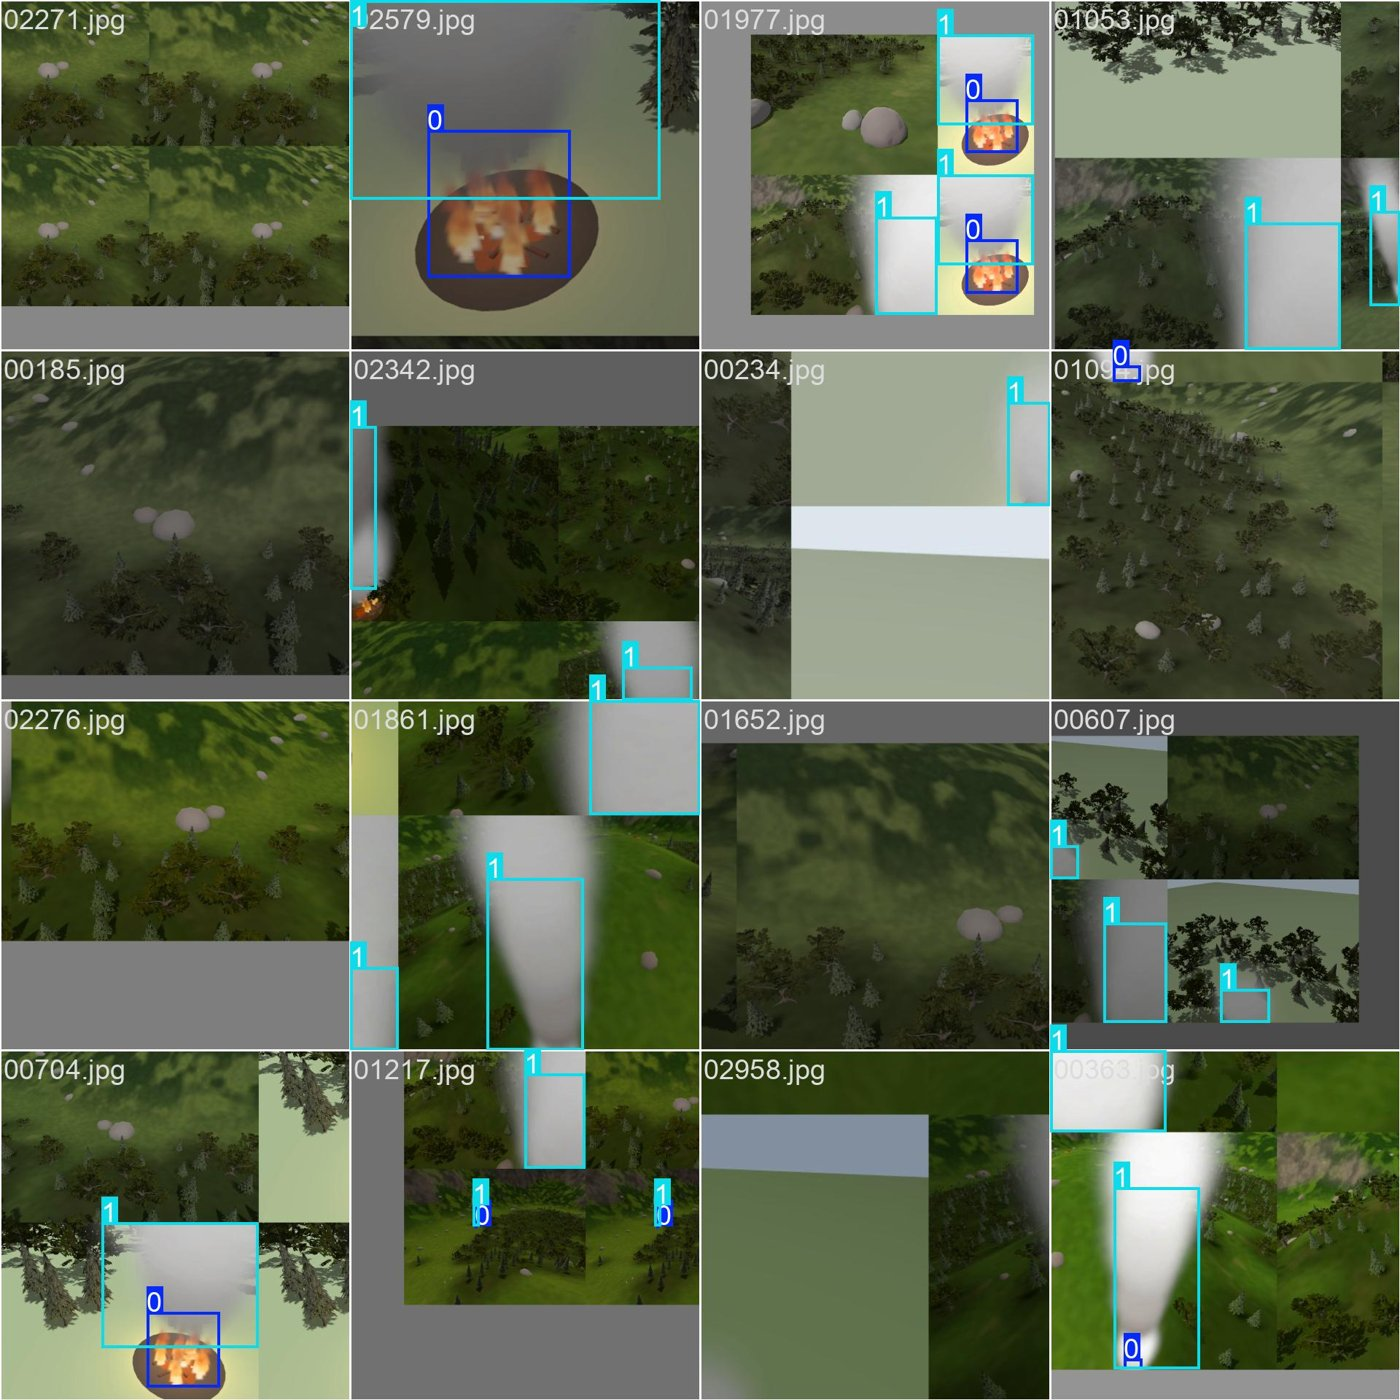
\includegraphics[width=0.85\textwidth]{yolo_lote_etiquetas.jpg}
\caption{Un lote de imágenes de entrenamiento con sus etiquetas. Las imágenes se alteran al azar
(mosaicos, cambios de color y escala) para que la red no memorice.}
\end{figure}

\begin{tecnico}
Etiquetar 6000 imágenes a mano tomaría días. Como en el simulador sabemos dónde está el fuego, las
etiquetas se calcularon solas: se proyecta con el modelo estenopeico una nube de puntos del volumen de
las llamas y del humo, se descartan los puntos tapados por árboles o por el terreno, y la caja es el
rectángulo que encierra los puntos visibles (capítulo~\ref{cap:yolo-sim}).
\end{tecnico}

\section{Cómo se mide si funciona}

\subsection{IoU: ¿le atinó a la caja?}

Una predicción cuenta como acierto si su caja se parece lo bastante a la verdadera. Se mide con la
\textbf{intersección sobre unión} (IoU):

\begin{figure}[H]
\centering
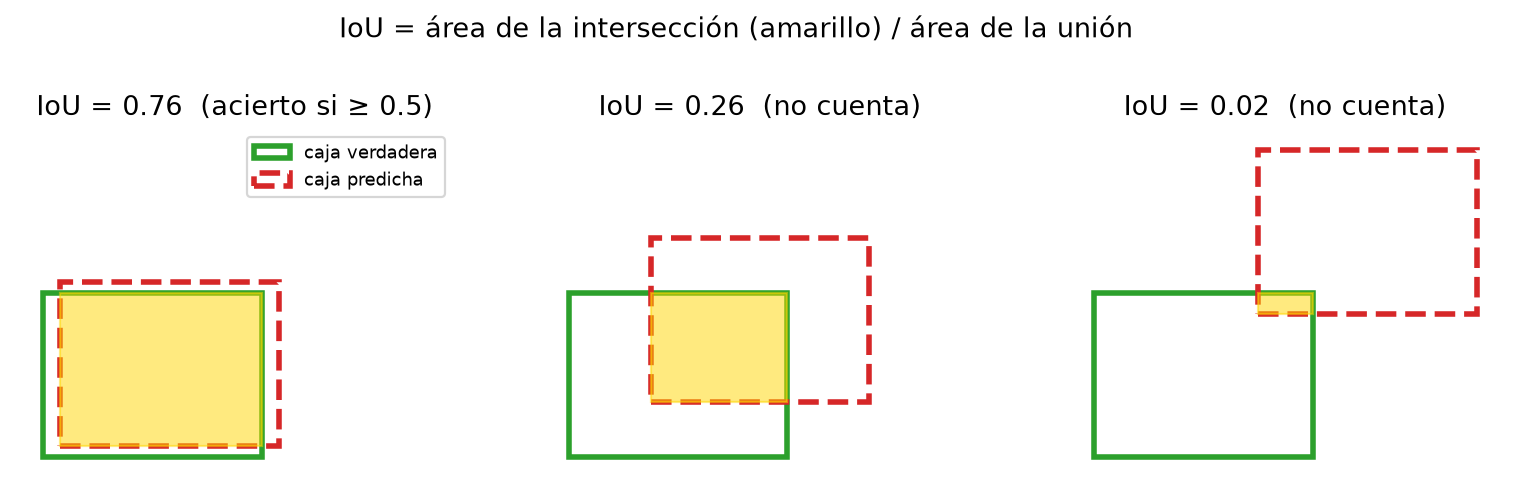
\includegraphics[width=\textwidth]{c_iou.png}
\caption{IoU: 1 es perfecta, 0 es no tocarse. Normalmente se exige al menos 0.5.}
\end{figure}

\subsection{Precisión y recall}

\begin{description}
  \item[Verdadero positivo (VP):] dijo ``fuego'' y había fuego.
  \item[Falso positivo (FP):] dijo ``fuego'' y no había (por ejemplo, una roca oscura).
  \item[Falso negativo (FN):] había fuego y no lo vio.
\end{description}
\begin{align}
\text{precisión} &= \frac{VP}{VP + FP} && \text{(cuando dice ``fuego'', ¿cuántas veces acierta?)}\\
\text{recall} &= \frac{VP}{VP + FN} && \text{(de los fuegos que hay, ¿cuántos encuentra?)}
\end{align}

\begin{ejemplo}
Una alarma de humo muy sensible tiene buen recall (no se le escapa ningún incendio) pero mala precisión
(suena cuando quemas pan tostado). Una muy poco sensible, al revés. Para un dron que vigila un bosque
importan las dos: no queremos ignorar un incendio, pero tampoco mandar a los bomberos a ver una roca.
\end{ejemplo}

\subsection{mAP}

La \textbf{precisión media} (AP) resume la curva de precisión contra recall al variar el umbral de
confianza; promediada entre clases es la \textbf{mAP}. \emph{mAP50} usa IoU $\ge$ 0.5; \emph{mAP50-95}
promedia exigencias de IoU de 0.5 a 0.95 (cajas más ajustadas). Nuestro modelo final: mAP50 = 0.988 y
mAP50-95 = 0.881, precisión 0.97 y recall 0.95.

\begin{figure}[H]
\centering
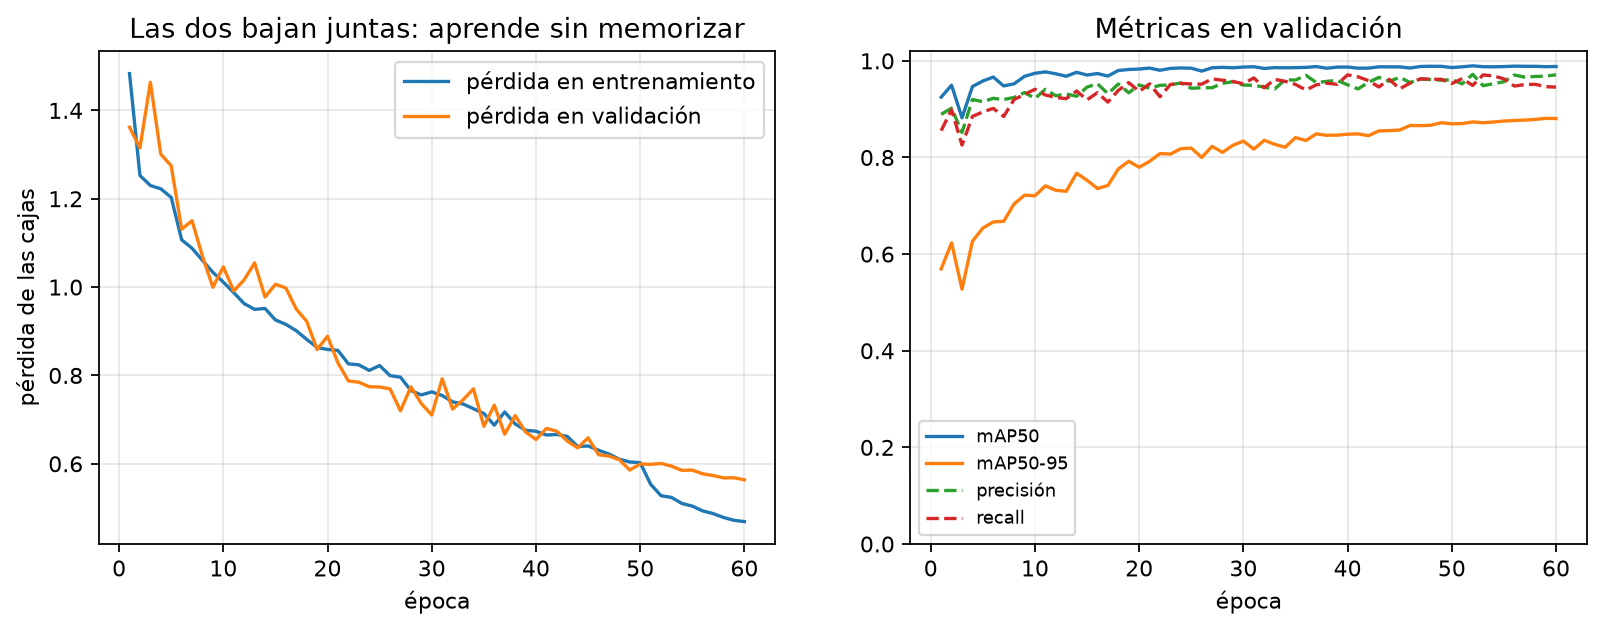
\includegraphics[width=\textwidth]{c_entrenamiento.png}
\caption{Izquierda: la pérdida baja en entrenamiento y en validación a la par (no hay
sobreajuste). Derecha: las métricas suben y se estabilizan.}
\end{figure}

\section{Sobreajuste y por qué importan los datos}

Si la red memoriza las imágenes de entrenamiento en lugar de aprender el concepto, le va muy bien con
ellas y mal con imágenes nuevas: eso es \textbf{sobreajuste}. Se detecta porque la pérdida de
validación deja de bajar o sube. Más importante aún: \textbf{la red solo sabe lo que vio}.

\begin{leccion}
El primer modelo se entrenó solo con el mundo \cod{bosque} (plano, sin rocas grandes). En el mundo
grande confundió una roca oscura con fuego: nunca había visto una roca. Se agregaron 3000 imágenes del
mundo grande, una de cada cinco apuntando a rocas o animales sin fuego, y el problema desapareció.
\end{leccion}

\begin{aviso}
Un modelo entrenado solo con imágenes de simulación probablemente fallará con fuego real: los colores,
la luz y el humo reales son distintos. Antes de volar el dron de verdad hay que reentrenar con imágenes
reales (por ejemplo, el dataset D-Fire).
\end{aviso}

\chapter{El detector de incendios de la simulación}
\label{cap:yolo-sim}

\begin{enpocas}
Cómo se generaron las 6000 imágenes etiquetadas, cómo se entrenó YOLO26n, qué tan bien quedó y cómo
funciona el nodo que detecta fuego y humo durante el vuelo.
\end{enpocas}

\section{Por qué ajustar un modelo}

YOLO26 es la última versión publicada de Ultralytics. Los modelos preentrenados en COCO no tienen
clases de fuego ni de humo, así que se ajustó \textbf{YOLO26n} (el más rápido de la familia,
adecuado para un dron) con imágenes del propio simulador, etiquetadas automáticamente. Las clases
son \emph{fuego} y \emph{humo}.

\section{Captura del dataset}

\cod{scripts/capturar_dataset.py} abre el mundo sin dron, con una cámara de la misma óptica que la
del dron (640$\times$480, HFOV 1.3~rad), y repite: mueve el foco y la cámara a posiciones al azar,
toma una imagen y la etiqueta. Para etiquetar proyecta con el modelo de cámara estenopeica una
nube de puntos del volumen de las llamas y de la columna de humo; descarta los puntos que tapan las
copas de los árboles (y, en el mundo grande, el relieve), así que cada caja cubre solo la parte
visible.

\begin{lstlisting}[style=bash]
# Mundo 'bosque'
python3 scripts/capturar_dataset.py preparar /tmp/datos/bosque.sdf /tmp/cuadrirotor_sim_$UID/modelos
GZ_SIM_RESOURCE_PATH=/tmp/datos/modelos_captura:$PWD/models \
    gz sim -s -r --headless-rendering /tmp/datos/bosque.sdf &
python3 scripts/capturar_dataset.py capturar ~/datasets/incendio_bosque 3000

# Mundo 'bosque_grande' (relieve, rocas, animales, cielo y penacho alto)
python3 scripts/capturar_dataset.py preparar /tmp/datos/bg.sdf /tmp/cuadrirotor_sim_$UID/modelos bosque_grande
python3 scripts/capturar_dataset.py capturar ~/datasets/incendio_bosque_grande 3000 bosque_grande
\end{lstlisting}

En el mundo grande el foco se pone en cualquier punto del valle (se espera 30~s cada vez que se
mueve para que el humo se forme), y una de cada cinco tomas apunta a una roca o a un animal: son
ejemplos de lo que \emph{no} es fuego. Se capturaron 3000 imágenes en cada mundo; en el grande, 989
con fuego, 2111 con humo y 836 vacías.

\begin{leccion}
Con el primer modelo, entrenado solo con el bosque plano, una roca oscura de 2.6~m en
$(-129,-154)$ del mundo grande se detectaba como \emph{fuego}: se parece al suelo quemado del foco.
Se resolvió capturando el segundo dataset, con tomas dirigidas a rocas y animales, y reentrenando
con los dos juntos.
\end{leccion}

\section{Entrenamiento}

\begin{lstlisting}[style=bash]
~/.venvs/yolo/bin/python scripts/entrenar_yolo.py ~/datasets/incendio_bosque \
    ~/datasets/incendio_bosque_grande 60
\end{lstlisting}

El script combina los datasets (escribe \cod{~/datasets/combinado_.../data.yaml}), ajusta YOLO26n
partiendo de los pesos de COCO (60 épocas, lote de 32, imágenes de 640) en la GPU y copia el mejor
modelo a \cod{yolo/incendio_yolo26n.pt}. Resultado en el conjunto de validación: precisión 0.971,
\emph{recall} 0.946, \textbf{mAP50 = 0.988} y mAP50-95 = 0.881.

\begin{figure}[H]
\centering
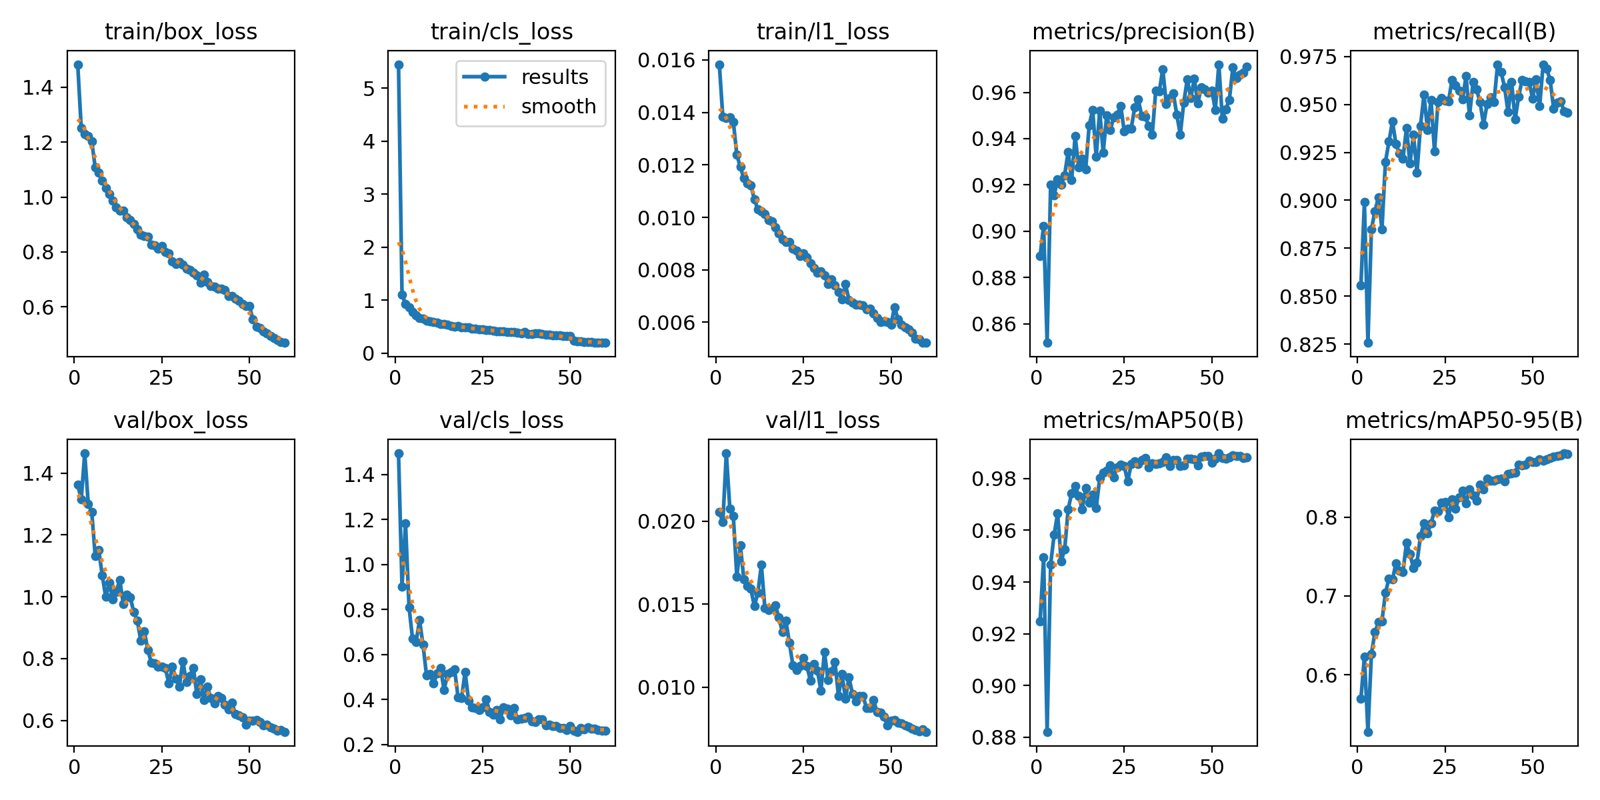
\includegraphics[width=\textwidth]{yolo_resultados.jpg}
\caption{Curvas de entrenamiento (pérdidas y métricas por época).}
\end{figure}

\begin{figure}[H]
\centering
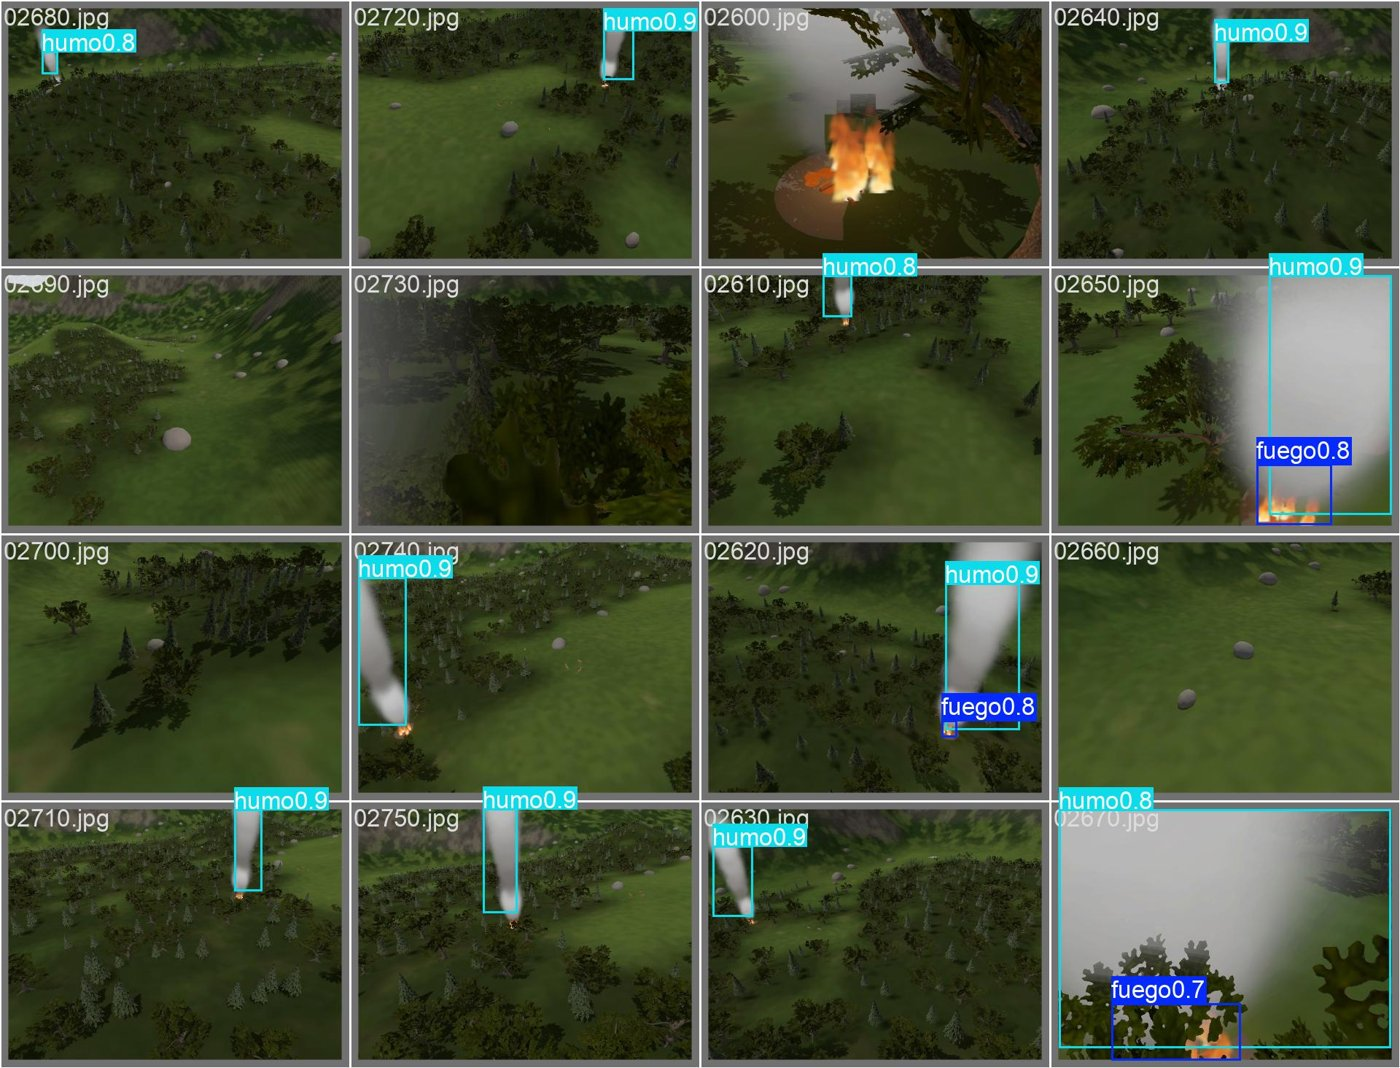
\includegraphics[width=0.8\textwidth]{yolo_val_pred.jpg}
\caption{Predicciones sobre imágenes de validación.}
\end{figure}

\begin{figure}[H]
\centering
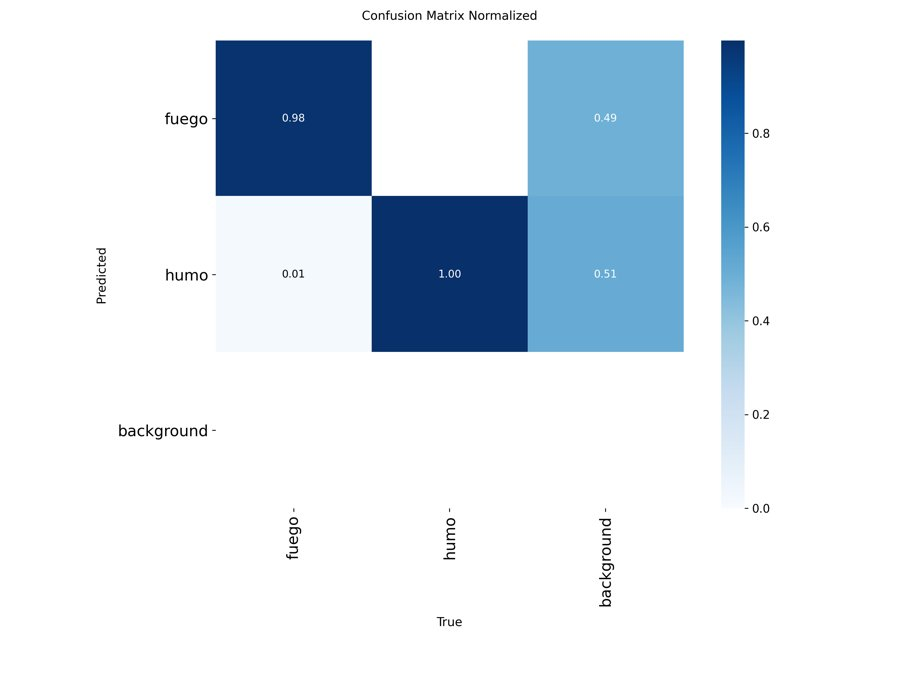
\includegraphics[width=0.55\textwidth]{yolo_confusion.jpg}
\caption{Matriz de confusión normalizada.}
\end{figure}

\section{El nodo detector}

\cod{detector_yolo.py} corre con el Python de \cod{~/.venvs/yolo}. Lee \cod{/cuadrirotor/camara},
corre el modelo en la GPU a $\approx$10~Hz y publica:
\begin{itemize}
  \item \cod{/cuadrirotor/detecciones} (\cod{vision_msgs/Detection2DArray}) con la marca de tiempo
        de la imagen, para emparejarla con la pose del dron en ese instante;
  \item \cod{/cuadrirotor/camara_yolo}: la imagen con las cajas dibujadas, que se ve en el panel
        ``Detección YOLO'' de Gazebo (\cod{config/gazebo_gui_yolo.config}).
\end{itemize}

\begin{figure}[H]
\centering
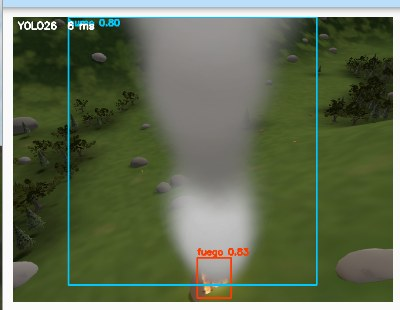
\includegraphics[width=0.5\textwidth]{yolo_panel.jpg}
\caption{Panel ``Detección YOLO'' durante la órbita: caja de \emph{humo} (cian) y de \emph{fuego}
(rojo) con su confianza.}
\end{figure}

\begin{nota}
Para volar con el dron real conviene volver a entrenar mezclando imágenes reales de incendios
(por ejemplo, el dataset D-Fire) con las del simulador.
\end{nota}


\part{Construir la simulación}
\chapter{Instalación paso a paso}
\label{cap:instalacion}

\begin{enpocas}
Qué hay que instalar y en qué orden: ROS~2 y Gazebo, el espacio de trabajo con nuestros paquetes, ArduPilot, el entorno de YOLO y las herramientas de CAD. Cada paso es un script que ya quedó en la carpeta personal.
\end{enpocas}

La instalación se hizo con cuatro scripts que quedaron en la carpeta personal
(\cod{~/instalar_ros2_gazebo.sh}, \cod{~/instalar_ardupilot.sh}, \cod{~/instalar_vision_yolo.sh}
y \cod{~/ardupilot_sitl.sh}). Esta sección explica qué hace cada uno y en qué orden se corren.

\section{ROS 2 Jazzy y Gazebo Harmonic}

\begin{lstlisting}[style=bash]
sudo bash ~/instalar_ros2_gazebo.sh
\end{lstlisting}

El script:
\begin{enumerate}
  \item agrega el repositorio \emph{universe} y el paquete \cod{ros2-apt-source} (que configura
        el repositorio oficial de ROS~2 para Ubuntu Noble);
  \item instala \cod{ros-jazzy-desktop}, \cod{ros-dev-tools}, el puente \cod{ros-jazzy-ros-gz}
        (trae Gazebo Harmonic), \cod{ros-jazzy-actuator-msgs}, \cod{ros-jazzy-xacro},
        PlotJuggler, el almacenamiento MCAP de \emph{rosbag2}, \cod{colcon} y numpy, scipy,
        matplotlib y pandas;
  \item inicializa \cod{rosdep}.
\end{enumerate}

Después, en cada terminal (o en \cod{~/.bashrc}):
\begin{lstlisting}[style=bash]
source /opt/ros/jazzy/setup.bash
\end{lstlisting}

Comprobación rápida: \cod{gz sim shapes.sdf} debe abrir Gazebo con unas figuras, y
\cod{ros2 topic list} debe responder.

\section{Espacio de trabajo}

\begin{lstlisting}[style=bash]
git clone https://github.com/jairoroke/Monitoreo-de-incendios-en-un-vehiculo-aereo-no-tripulado.git ~/ros2_ws
# Solo para controlador:=ardupilot (plugin de ArduPilot para Gazebo):
git clone https://github.com/ArduPilot/ardupilot_gazebo.git ~/ros2_ws/src/ardupilot_gazebo

cd ~/ros2_ws
export GZ_VERSION=harmonic
colcon build --symlink-install
source install/setup.bash
\end{lstlisting}

\cod{--symlink-install} enlaza los archivos de Python, los \emph{launch} y los YAML en lugar de
copiarlos: un cambio en \cod{src/} se ve sin volver a compilar (hay que recompilar solo si se
agrega un ejecutable nuevo en \cod{setup.py} o se cambia código C++). El espacio tiene dos
paquetes propios:

\begin{description}
  \item[\cod{cuadrirotor_sim}] (Python, \emph{ament\_python}): modelos, mundos, controladores,
        planificador, detector, \emph{launch}, scripts y pruebas.
  \item[\cod{cuadrirotor_gz_plugins}] (C++): dos sistemas de Gazebo, \cod{FuerzaViento} (fuerza
        externa de viento) y \cod{ComandosMotores} (para ArduPilot, sección~\ref{sec:plugin-ap}).
\end{description}

\section{ArduPilot SITL}
\label{sec:inst-ardupilot}

ArduCopter 4.7.2 se compila para SITL (\emph{software in the loop}) en \cod{~/ardupilot}:

\begin{lstlisting}[style=bash]
git clone --recurse-submodules https://github.com/ArduPilot/ardupilot.git ~/ardupilot
cd ~/ardupilot && git checkout Copter-4.7.2 && git submodule update --init --recursive
bash ~/instalar_ardupilot.sh          # como usuario normal, NO con sudo
./waf configure --board sitl && ./waf copter
\end{lstlisting}

\cod{instalar_ardupilot.sh} corre \cod{Tools/environment_install/install-prereqs-ubuntu.sh}
con dos variables que evitan conflictos con ROS:
\cod{DO_PYTHON_VENV_ENV=0} (no activar el entorno de Python de ArduPilot en cada terminal; chocaría
con el \cod{python3} de ROS) y \cod{DO_AP_STM_ENV=0} (no instalar el compilador para placas STM32).
Crea el entorno \cod{~/venv-ardupilot} con MAVProxy y pymavlink, e instala las bibliotecas de
GStreamer que necesita el plugin \cod{ardupilot_gazebo}. El binario queda en
\cod{~/ardupilot/build/sitl/bin/arducopter}.

En \cod{~/.bashrc} quedaron:
\begin{lstlisting}[style=bash]
export GZ_VERSION=harmonic
export GZ_SIM_SYSTEM_PLUGIN_PATH=$HOME/ros2_ws/install/ardupilot_gazebo/lib/ardupilot_gazebo:${GZ_SIM_SYSTEM_PLUGIN_PATH}
export GZ_SIM_RESOURCE_PATH=$HOME/ros2_ws/install/ardupilot_gazebo/share/ardupilot_gazebo/models:$HOME/ros2_ws/install/ardupilot_gazebo/share/ardupilot_gazebo/worlds:${GZ_SIM_RESOURCE_PATH}
export PATH=$HOME/ardupilot/Tools/autotest:$PATH
\end{lstlisting}

Prueba del SITL con el Iris de ejemplo (sin nuestra simulación):
\begin{lstlisting}[style=bash]
bash ~/ardupilot_sitl.sh              # iris_runway.sdf + sim_vehicle.py --console --map
\end{lstlisting}

Para la ventana que acomoda las ventanas del SITL (sección~\ref{sec:ventanas}) se agregó
\cod{python-xlib} al entorno de ArduPilot:
\begin{lstlisting}[style=bash]
~/venv-ardupilot/bin/pip install python-xlib
\end{lstlisting}

\section{Visión: YOLO26}

\begin{lstlisting}[style=bash]
bash ~/instalar_vision_yolo.sh        # descarga ~3 GB
\end{lstlisting}

Crea \cod{~/.venvs/yolo} con \cod{--system-site-packages} (el detector necesita ver los paquetes de
ROS~2) e instala \cod{ultralytics} con PyTorch y CUDA. Fija tres versiones:
\begin{itemize}
  \item \cod{numpy<2}: los mensajes de ROS~2 Jazzy están compilados con numpy 1.x;
  \item \cod{opencv-python<4.12}: las versiones nuevas exigen numpy 2;
  \item \cod{setuptools<80}: lo que acepta \cod{colcon}.
\end{itemize}
Al final comprueba que PyTorch vea la GPU y que \cod{rclpy} se importe desde el entorno.

\section{Herramientas de CAD y generación de mundos}

La conversión del CAD del Tarot y la generación del terreno usan bibliotecas que no vienen con
ROS. Van en un entorno aparte:
\begin{lstlisting}[style=bash]
python3 -m venv --without-pip ~/.venvs/cad
curl -sSL https://bootstrap.pypa.io/get-pip.py | ~/.venvs/cad/bin/python
~/.venvs/cad/bin/pip install cascadio trimesh numpy fast_simplification pillow scipy matplotlib
\end{lstlisting}

\begin{nota}
Se intentó primero convertir el STEP con \emph{gmsh}, pero tardaba más de 15 minutos;
\cod{cascadio} (teselador de OpenCASCADE) con \cod{trimesh} lo hace en segundos.
\end{nota}

\section{Comprobación de la instalación}

\begin{lstlisting}[style=bash]
cd ~/ros2_ws/src/cuadrirotor_sim && python3 -m pytest -q test/     # 31 pruebas
ros2 launch cuadrirotor_sim simulacion.launch.py                    # cuadrirrotor en hover
\end{lstlisting}

\chapter{Dónde está cada cosa: el espacio de trabajo}

\begin{enpocas}
Un mapa de las carpetas y archivos del proyecto, para saber dónde buscar cuando quieras cambiar algo.
\end{enpocas}

\begin{lstlisting}
~/ros2_ws/
|-- README.md                      descripción y órdenes (resumen de este manual)
`-- src/
    |-- cuadrirotor_sim/           paquete principal (Python)
    |   |-- cuadrirotor_sim/       nodos y bibliotecas
    |   |-- launch/simulacion.launch.py
    |   |-- config/                parámetros (YAML), GUI de Gazebo, ArduPilot
    |   |-- models/                vehículos, árboles, fauna, fuego, terreno
    |   |-- worlds/                incendio.sdf, bosque.sdf, bosque_grande.sdf
    |   |-- scripts/               generadores, captura de datos, entrenamiento
    |   |-- yolo/incendio_yolo26n.pt   pesos del detector
    |   `-- test/                  pruebas (pytest)
    |-- cuadrirotor_gz_plugins/    sistemas de Gazebo en C++
    `-- ardupilot_gazebo/          plugin de ArduPilot (clonado)
\end{lstlisting}

\section{Módulos del paquete \texorpdfstring{\texttt{cuadrirotor\_sim}}{cuadrirotor\_sim}}

\begin{longtable}{>{\raggedright\arraybackslash}p{4.2cm}p{11cm}}
\toprule
\textbf{Archivo} & \textbf{Qué hace} \\ \midrule \endhead
\cod{dinamica.py} & Rotaciones, mezclador de rotores (empuje y pares $\rightarrow$ velocidades), referencia de las misiones \emph{hover} y \emph{órbita}. \\
\cod{controlador_pd.py} & Nodo del PD en cascada: lazo de posición y PD sobre SO(3). Base de los demás controladores. \\
\cod{sta.py} & Super-twisting adaptativo con discretización explícita, semi-implícita e implícita. \\
\cod{controlador_sta.py} & Nodo que reemplaza el lazo de posición del PD por el STA. \\
\cod{viento.py} & Perturbación $F(t)=F_0+A\sin(2\pi f t)$ publicada en \cod{/cuadrirotor/viento}. \\
\cod{terreno.py} & Modelo digital de elevación (DEM): altura, máximo en un tramo y corte de rayos. \\
\cod{bosque_grande.py} & Arma el SDF del mundo grande con el foco donde se pida. \\
\cod{fauna.py} & Mueve a los animales (pastar, caminar, trotar) por gz-transport. \\
\cod{detector_yolo.py} & YOLO26n sobre la cámara; publica cajas y la imagen anotada. \\
\cod{busqueda_incendio.py} & Planificador autónomo: máquina de estados de la búsqueda. \\
\cod{cobertura.py} & Rutas de barrido (franjas y serpentina) y mapa de cobertura. \\
\cod{evasion.py} & Evasión reactiva de obstáculos con el LiDAR (histograma polar). \\
\cod{geo.py} & Conversión del marco del mundo (ENU) a coordenadas GPS (WGS84). \\
\cod{mision_ardupilot.py} & Misión por MAVLink para ArduCopter SITL. \\
\cod{ventanas_sitl.py} & Acomoda las ventanas del SITL en la pantalla. \\
\cod{mavproxy_trayectoria.py} & Módulo de MAVProxy: dibuja la trayectoria, la ruta y el foco en el mapa. \\
\bottomrule
\end{longtable}

\section{Scripts}

\begin{longtable}{>{\raggedright\arraybackslash}p{4.6cm}p{10.6cm}}
\toprule
\textbf{Script} & \textbf{Uso} \\ \midrule \endhead
\cod{cad_a_malla.py} & Convierte el STEP del Tarot en mallas STL por grupos de piezas. \\
\cod{generar_modelo.py} & Escribe el SDF de cada vehículo y su YAML desde una sola tabla de parámetros. \\
\cod{generar_fuego.py} & Texturas de las partículas y modelos \cod{foco_incendio} y \cod{columna_humo}. \\
\cod{generar_bosque.py} & Mundo \cod{bosque} (85 árboles, semilla fija). \\
\cod{generar_bosque_grande.py} & Terreno, textura, árboles, rocas, fauna y DEM del mundo grande. \\
\cod{preparar_fauna.py} & Descarga y adapta los modelos CC0 de venado, zorro y lobo. \\
\cod{capturar_dataset.py} & Genera imágenes etiquetadas para YOLO desde Gazebo. \\
\cod{entrenar_yolo.py} & Ajusta YOLO26n con uno o varios datasets. \\
\cod{corrida.sh}, \cod{metricas.py} & Campañas de simulación y métricas (RMS, máximo, \emph{chattering}). \\
\bottomrule
\end{longtable}

\section{Archivos de configuración}

\begin{description}
  \item[\cod{config/parametros.yaml}] misión por omisión (altura, foco, radio, $\omega$), ganancias del PD
        y del STA, y viento.
  \item[\cod{config/vehiculo_<vehiculo>.yaml}] masa, inercia, rotores, $k_f$, $k_m$, $\omega_{max}$, lazo de
        actitud y cámara. Lo genera \cod{generar_modelo.py}: no se edita a mano.
  \item[\cod{config/mundo_bosque_grande.yaml}] parámetros de la búsqueda en el mundo grande.
  \item[\cod{config/puente.yaml}] tópicos que cruza \cod{ros_gz_bridge} entre Gazebo y ROS~2.
  \item[\cod{config/ardupilot/tarot650.parm}] parámetros de ArduCopter para el Tarot.
  \item[\cod{config/gazebo_gui*.config}] distribución de la ventana de Gazebo (con el panel de la
        cámara o el de detección de YOLO).
\end{description}

\begin{aviso}
Los \cod{-p clave:=valor} de la línea de comandos \textbf{no} sobrescriben lo que esté en la
sección de un nodo dentro del YAML (el YAML del nodo tiene prioridad). Para campañas se usa
\cod{scripts/corrida.sh}, que genera un YAML de ajustes.
\end{aviso}

\chapter{Cómo se metió el Tarot 650 en Gazebo}

\begin{enpocas}
Cómo se pasó el dron de un archivo CAD a un modelo que vuela en Gazebo: las mallas, la tabla de parámetros, los motores, el mezclador, los sensores y el viento.
\end{enpocas}

\begin{figure}[H]
\centering
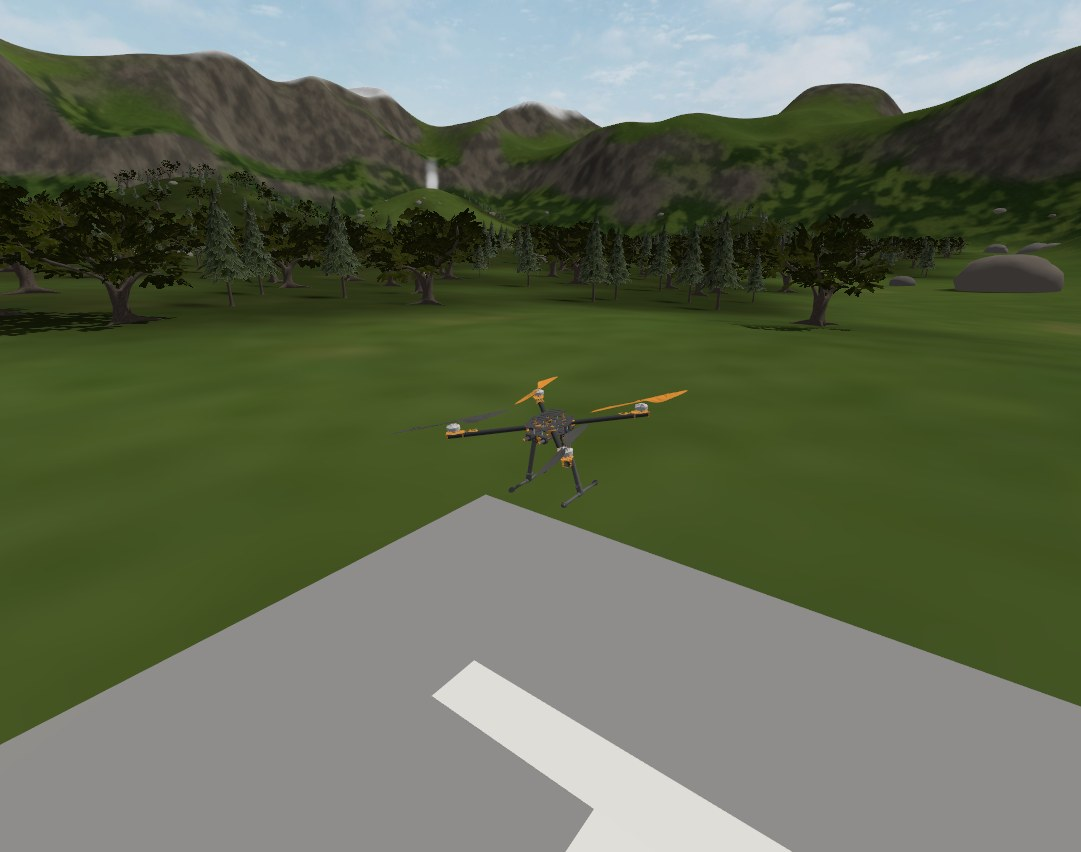
\includegraphics[width=0.78\textwidth]{gz_tarot_cerca.jpg}
\caption{El Tarot 650 en vuelo estacionario sobre la base de despegue del mundo
\cod{bosque_grande}. Las hélices delanteras son naranjas.}
\label{fig:tarot-gz}
\end{figure}

\section{Del CAD a las mallas}

La geometría viene del modelo de GrabCAD \emph{Tarot Ironman 650}
(\url{https://grabcad.com/library/tarot-ironman-650-2}), con motores T-Motor MN3508 y hélices
de $15\times5$''. El archivo \cod{Tarot.stp} es un ensamble de cientos de piezas. Se convirtió
con \cod{scripts/cad_a_malla.py} en dos pasos:

\begin{lstlisting}[style=bash]
# 1) Ver las piezas: nombre, cuántas hay y su tamaño
~/.venvs/cad/bin/python scripts/cad_a_malla.py listar "Tarot 650/Tarot.stp"

# 2) Exportar grupos de piezas por nombre (expresiones regulares)
~/.venvs/cad/bin/python scripts/cad_a_malla.py exportar "Tarot 650/Tarot.stp" salida/ \
    --grupo placas='Base$|base|side bracket|lower support|bracket landing' \
    --grupo brazos='CarbonArm' \
    --grupo acentos='orange|clamp|pivot|clip|Motortoarm|ArmCopter|cap' \
    --grupo tren='Lower Tube|leg|foot|landing-gear|Landing' --grupo motores='bell' \
    --grupo marco=resto --excluir '94180|bearing|circlip|coil|axle|stator|15x5' \
    --ejes +z +x +y --origen 0.0142 0 0.0070

# Hélices, cada una por aparte y centrada:
~/.venvs/cad/bin/python scripts/cad_a_malla.py exportar "Tarot 650/Tarot.stp" salida/ \
    --grupo helice='15x5' --separar helice --caras 4000 --ejes +z +x +y --origen 0.0142 0 0.0070
\end{lstlisting}

\begin{itemize}
  \item \cod{--ejes +z +x +y} dice qué eje del CAD es el \emph{x} (frente), el \emph{y}
        (izquierda) y el \emph{z} (arriba) del modelo. El frente quedó paralelo a los patines del
        tren de aterrizaje.
  \item \cod{--origen} es el punto del CAD (en metros) que queda en el origen del cuerpo.
  \item Cada grupo se exporta como un STL con su color en el SDF: placas y brazos de carbono,
        acentos naranjas, tren, campanas de los motores y el resto del marco.
  \item \cod{helice_i.stl} se asigna al rotor $i$ por su posición.
\end{itemize}

\begin{aviso}
No se deben simplificar \cod{placas} ni \cod{brazos}: las placas de carbono miden 1.6~mm y la
simplificación de la malla las deshace. Sí se pueden reducir \cod{acentos} (50\,000 caras),
\cod{tren} (25\,000) y \cod{motores} (20\,000).
\end{aviso}

\begin{figure}[H]
\centering
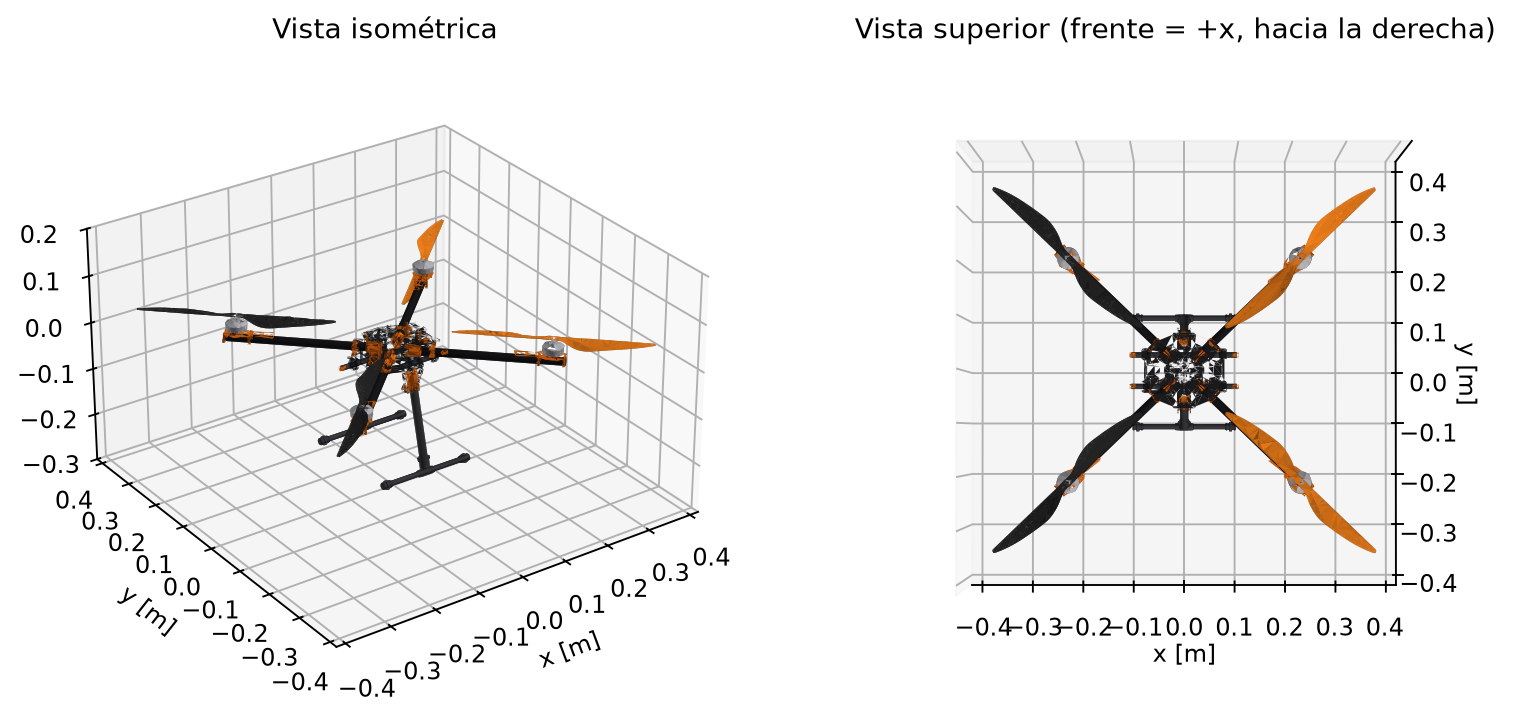
\includegraphics[width=\textwidth]{tarot_render.png}
\caption{Mallas del Tarot convertidas del CAD (\cod{models/tarot650/meshes}), en el marco del
cuerpo.}
\end{figure}

\section{Parámetros del vehículo}

Todos los parámetros están en una sola tabla, \cod{VEHICULOS} de \cod{scripts/generar_modelo.py}.
De ella salen la planta que simula Gazebo (\cod{models/tarot650/model.sdf}) y los valores que usa
el controlador (\cod{config/vehiculo_tarot650.yaml}), así que el modelo del controlador coincide
siempre con la planta. Para cambiar un parámetro se edita la tabla y se vuelve a correr:

\begin{lstlisting}[style=bash]
python3 scripts/generar_modelo.py            # todos los vehículos
python3 scripts/generar_modelo.py tarot650   # solo uno
\end{lstlisting}

\begin{table}[H]
\centering\small
\begin{tabular}{lll}
\toprule
\textbf{Parámetro} & \textbf{Valor} & \textbf{Origen} \\ \midrule
Configuración & ``X'', 4 rotores & CAD \\
Posición de los rotores $(x_i, y_i)$ & $(\pm0.2198,\ \pm0.212)$~m & CAD \\
Altura de los rotores & 0.04~m sobre el origen & CAD \\
Tren de aterrizaje & dos patines a lo largo de \emph{x}, 0.2205~m bajo el origen & CAD \\
Radio de la hélice & 0.1905~m (15'') & CAD \\
Masa total & 2.2~kg (cuerpo 2.12 + 4 rotores de 0.02) & supuesto \\
Inercia total $J$ & diag(0.03412, 0.03609, 0.06596)~kg\,m$^2$ & estimada \\
Constante de empuje $k_f$ & $4.24\times10^{-5}$~N/(rad/s)$^2$ & supuesto \\
Constante de par $k_m$ & 0.016~m & supuesto \\
Velocidad máxima $\omega_{max}$ & 680~rad/s ($\approx$ 19.6~N por motor) & supuesto \\
Constante de tiempo del motor & 30~ms al subir, 50~ms al bajar & supuesto \\
Velocidad en vuelo estacionario & 357~rad/s & calculada \\
Lazo de actitud $K_R$, $K_\omega$ & (3.4, 3.6, 1.65), (0.55, 0.58, 0.59) & ajustado \\
Cámara & 640$\times$480, 15~Hz, HFOV 1.3~rad, 30° hacia abajo & diseño \\
LiDAR 3D & 360°$\times$120 haces, 16 canales ($-35^\circ$ a $+15^\circ$), 30~m, 10~Hz & diseño \\
\bottomrule
\end{tabular}
\caption{Parámetros del Tarot 650 en la simulación.}
\label{tab:tarot}
\end{table}

\begin{aviso}
La geometría es la del CAD, pero la masa, las inercias, $k_f$, $k_m$ y los retardos son valores
típicos supuestos para esta configuración. \textbf{Hay que reemplazarlos por los del dron real}
(peso con batería, KV de los motores, hélice, número de celdas) antes de sacar conclusiones
cuantitativas.
\end{aviso}

\section{Motores y mezclador}

Cada rotor es un \cod{MulticopterMotorModel} de Gazebo: recibe una velocidad de referencia
(\cod{/cuadrirotor/command/motor_speed}, un mensaje \cod{Actuators} con las cuatro velocidades),
la filtra con un sistema de primer orden y produce el empuje $f_i = k_f\,\omega_i^2$ y el par de
arrastre $k_m f_i$. Fragmento del SDF generado para el rotor 0:

\begin{lstlisting}[style=xml]
<plugin filename="gz-sim-multicopter-motor-model-system"
        name="gz::sim::systems::MulticopterMotorModel">
  <robotNamespace>cuadrirotor</robotNamespace>
  <jointName>rotor_0_joint</jointName>
  <linkName>rotor_0</linkName>
  <turningDirection>ccw</turningDirection>
  <timeConstantUp>0.03</timeConstantUp>
  <timeConstantDown>0.05</timeConstantDown>
  <maxRotVelocity>680.0</maxRotVelocity>
  <motorConstant>4.24e-05</motorConstant>
  <momentConstant>0.016</momentConstant>
  <commandSubTopic>command/motor_speed</commandSubTopic>
  <motorNumber>0</motorNumber>
  <rotorDragCoefficient>8.06428e-05</rotorDragCoefficient>
  <rollingMomentCoefficient>1e-06</rollingMomentCoefficient>
  <motorSpeedPubTopic>motor_speed/0</motorSpeedPubTopic>
  <rotorVelocitySlowdownSim>10</rotorVelocitySlowdownSim>
  <motorType>velocity</motorType>
</plugin>
\end{lstlisting}

\begin{figure}[H]
\centering
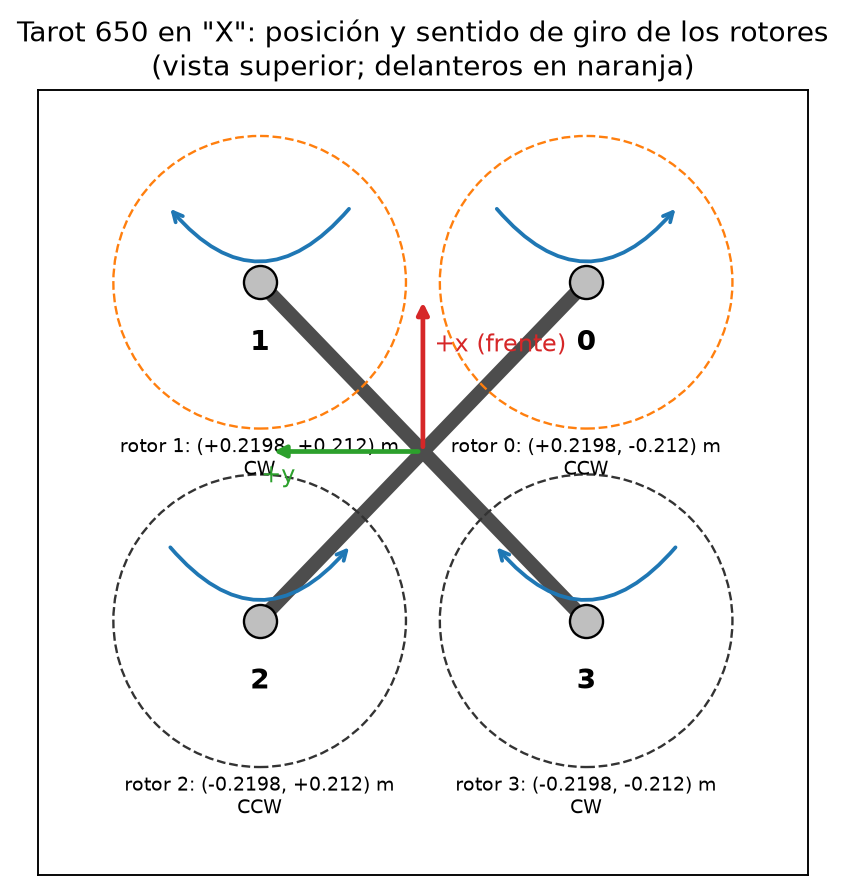
\includegraphics[width=0.62\textwidth]{tarot_planta.png}
\caption{Numeración, posición y sentido de giro de los rotores del Tarot.}
\label{fig:planta}
\end{figure}

El controlador calcula un empuje total $T$ y un par $\tau=(\tau_x,\tau_y,\tau_z)$. El mezclador
(\cod{dinamica.Mezclador}) los convierte en velocidades de rotor. Con el rotor $i$ en
$(x_i,y_i)$ y sentido $s_i$ ($+1$ antihorario, $-1$ horario):
\begin{equation}
\begin{bmatrix} T\\ \tau_x\\ \tau_y\\ \tau_z \end{bmatrix} =
\underbrace{\begin{bmatrix}
1 & 1 & 1 & 1\\
y_0 & y_1 & y_2 & y_3\\
-x_0 & -x_1 & -x_2 & -x_3\\
-s_0 k_m & -s_1 k_m & -s_2 k_m & -s_3 k_m
\end{bmatrix}}_{B}
\begin{bmatrix} f_0\\ f_1\\ f_2\\ f_3 \end{bmatrix},
\qquad
\omega_i = \sqrt{\frac{\operatorname{sat}_{[0,\,f_{max}]}\big((B^{+}[T,\tau]^\top)_i\big)}{k_f}} .
\end{equation}

En vuelo estacionario cada motor carga un cuarto del peso:
\begin{equation}
f_h = \frac{mg}{4} = \frac{2.2\cdot 9.81}{4} = 5.40\ \text{N},\qquad
\omega_h = \sqrt{\frac{f_h}{k_f}} = 357\ \text{rad/s},\qquad
\frac{f_h}{f_{max}} = \Big(\frac{357}{680}\Big)^2 = 0.28 .
\end{equation}
La relación empuje/peso es $4\cdot19.6/21.6\approx3.6$.

\begin{figure}[H]
\centering
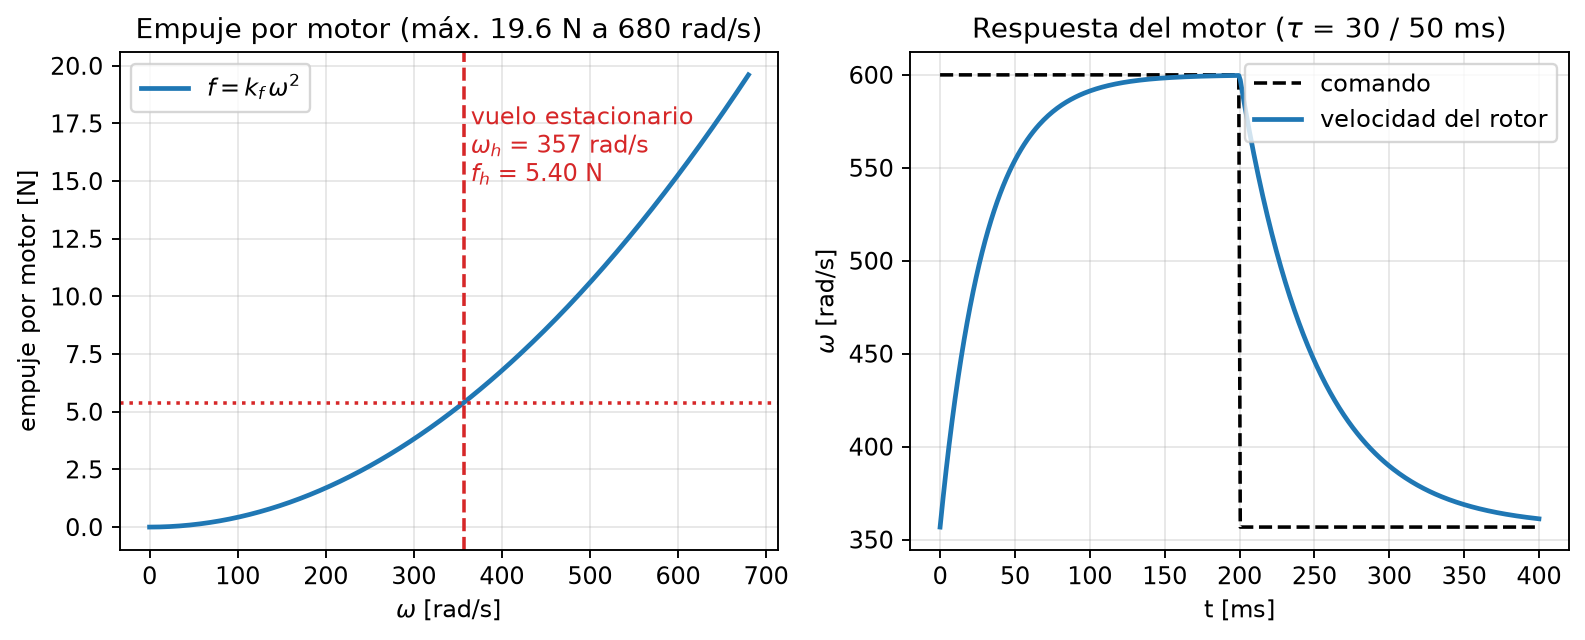
\includegraphics[width=\textwidth]{motor_empuje.png}
\caption{Curva de empuje de un motor y respuesta de primer orden a un escalón.}
\end{figure}

\section{Sensores}

\begin{description}
  \item[IMU] 200~Hz en \cod{/cuadrirotor/imu}.
  \item[Odometría] \cod{OdometryPublisher} a 1~kHz en \cod{/cuadrirotor/odometria} (posición y
        orientación verdaderas; velocidades en el marco del cuerpo).
  \item[Cámara frontal] inclinada 30° hacia abajo: ve el horizonte para buscar el humo de lejos y
        mantiene el foco a la vista en la órbita. Rango de recorte hasta 1500~m (antes 200~m) para
        que se vean las montañas.
  \item[LiDAR 3D] para la evasión de obstáculos (capítulo~\ref{cap:autonomia}):
\end{description}

\begin{lstlisting}[style=xml]
<sensor name="lidar" type="gpu_lidar">
  <pose>0 0 0.1 0 0 0</pose>
  <always_on>1</always_on>
  <update_rate>10</update_rate>
  <topic>cuadrirotor/lidar</topic>
  <lidar>
    <scan>
      <horizontal><samples>120</samples><min_angle>-3.14159</min_angle><max_angle>3.14159</max_angle></horizontal>
      <vertical><samples>16</samples><min_angle>-0.6109</min_angle><max_angle>0.2618</max_angle></vertical>
    </scan>
    <range><min>0.8</min><max>30</max><resolution>0.05</resolution></range>
  </lidar>
</sensor>
\end{lstlisting}

El alcance mínimo de 0.8~m evita que el LiDAR vea las propias hélices (las puntas quedan a
$\approx$0.5~m del centro). La nube llega a ROS como \cod{sensor_msgs/PointCloud2} en
\cod{/cuadrirotor/lidar/points}.

\section{Perturbación de viento}

El sistema \cod{FuerzaViento} (\cod{cuadrirotor_gz_plugins}) aplica sobre \cod{base_link} una fuerza
en el marco inercial y la mantiene en cada paso de física hasta que llega un valor nuevo; así la
perturbación es exactamente la señal publicada, sin acumularse. El nodo \cod{viento} publica
\begin{equation}
F(t) = F_0 + A\sin(2\pi f t),\qquad F_0 = 1\ \text{N},\ A = 0.5\ \text{N},\ f = 0.2\ \text{Hz},
\end{equation}
a partir de $t = 15$~s (con \cod{viento:=true}).

\chapter{Cómo se construyó el bosque}

\begin{enpocas}
Cómo se generaron por programa el terreno con montañas, su textura, los 1700 árboles, las rocas, los animales y el incendio con humo, y cómo los arma el \emph{launch} al arrancar.
\end{enpocas}

\section{Mundos disponibles}

\begin{description}
  \item[\cod{incendio}] terreno plano, tres árboles simples y el foco en $(8,5)$. Sirve para
        probar el control sin distracciones.
  \item[\cod{bosque}] como el del video de ArduPilot \cod{iris_forest}: 50 robles y 35 pinos de
        OpenRobotics (Gazebo Fuel, licencia CC0, copiados en \cod{models/roble} y
        \cod{models/pino} para funcionar sin internet) y el foco en $(8,5)$. Deja libres el
        despegue, el corredor al foco y el anillo de la órbita, así que la misión \cod{orbita}
        funciona a 3~m entre los árboles. Se genera con
        \cod{python3 scripts/generar_bosque.py worlds/bosque.sdf} (semilla fija).
  \item[\cod{bosque_grande}] el valle boscoso con montañas que se describe a continuación.
\end{description}

\section{El mundo \texorpdfstring{\texttt{bosque\_grande}}{bosque\_grande}}

\begin{figure}[H]
\centering
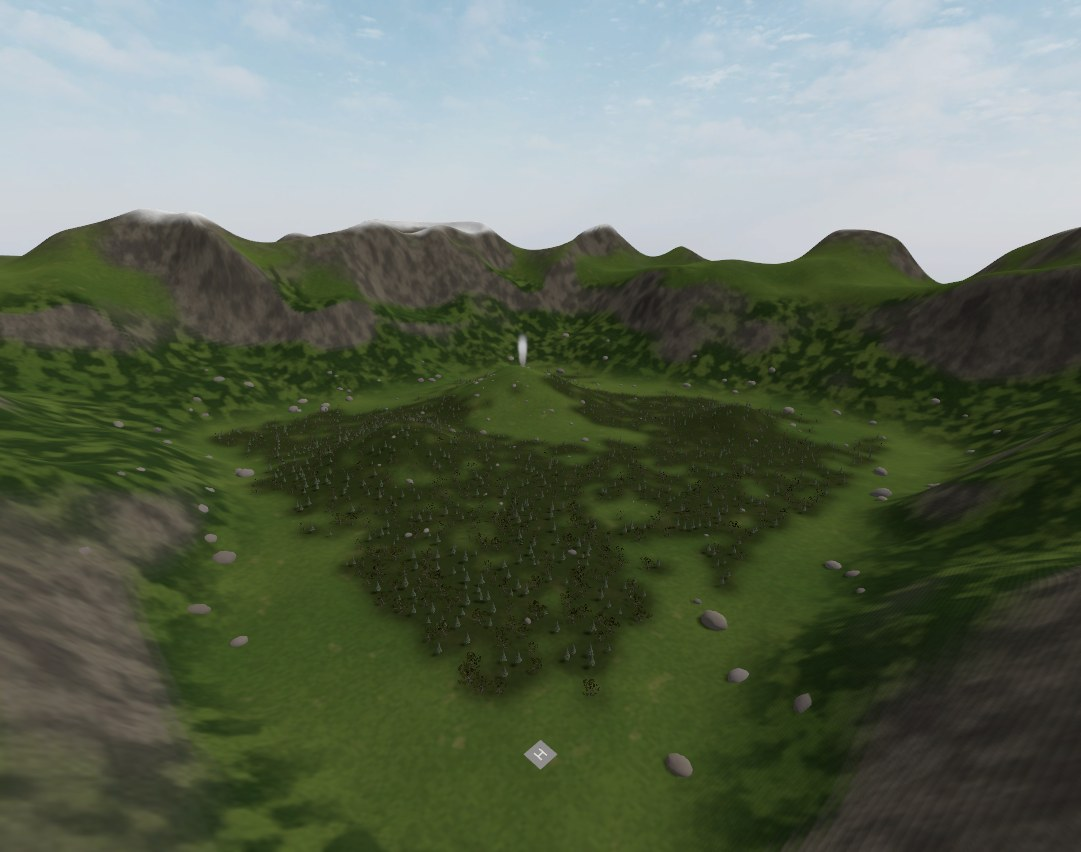
\includegraphics[width=\textwidth]{gz_valle_aereo.jpg}
\caption{Vista aérea del valle desde el suroeste. Abajo al centro, la base de despegue; al
fondo, el penacho de humo del incendio.}
\end{figure}

Se pidió ``un mundo más grande, con más árboles, montañas, piedras grandes, cielo y animales,
en el que el dron monitoree todo el bosque para encontrar el incendio''. El resultado:

\begin{itemize}
  \item Terreno de $1.2\times1.2$~km con malla de 4~m ($301\times301$ vértices). El valle mide
        $420\times420$~m, con lomas suaves y tres cerros de 18 a 42~m; alrededor, una cordillera
        de hasta $\approx$215~m con laderas de roca y nieve en las cumbres.
  \item Textura propia de $4096\times4096$ píxeles.
  \item 1700 árboles (956 pinos y 744 robles) de tamaños y orientaciones variables, con claros de
        pastizal; miden de 4.6 a 8.2~m.
  \item 140 rocas y peñascos.
  \item 21 animales (venados, lobos y zorros) que pastan y caminan.
  \item Cielo con nubes (\cod{<sky>} de Gazebo).
  \item Base de despegue de $8\times8$~m con una ``H'' en $(-232,-232)$, fuera del bosque.
  \item Foco de incendio por omisión en una ladera al noreste, $(105,135)$, con un claro
        quemado de 9~m y un penacho de humo de $\approx$30~m que se ve sobre las copas.
\end{itemize}

\subsection{Generación del terreno}

Todo lo genera una sola vez, con semilla fija (21), el script:
\begin{lstlisting}[style=bash]
~/.venvs/cad/bin/python scripts/generar_bosque_grande.py
\end{lstlisting}

\begin{enumerate}
  \item \textbf{Relieve} (\cod{alturas}). Suma de: ruido fractal suave de amplitud 7~m (lomas),
        tres gaussianas deformadas por ruido (los cerros), y la cordillera, que crece con la
        distancia al borde del valle. El borde es un cuadrado redondeado de 250~m de semilado
        ($|x|^6+|y|^6$) deformado por ruido para que no se vea artificial; las crestas salen de
        $1-|\text{ruido}|$. Se suaviza con un filtro gaussiano ($\sigma = 1.2$ celdas) y se aplana la
        base de despegue.
  \item \textbf{Textura} (\cod{colores_textura}). Por cada píxel: dos verdes de pasto mezclados con
        ruido, manchas secas, sotobosque oscuro bajo las copas (según la densidad de árboles),
        monte denso en las faldas, roca donde la pendiente pasa de $\approx$0.8 o la altura de
        140~m, y nieve por encima de 185~m.
  \item \textbf{Árboles} (\cod{distribuir_arboles}). Puntos al azar en la zona, descartando:
        cerca de las montañas (el bosque se ralea), en los claros (donde el ruido es bajo), a menos
        de 30~m de la base, con pendiente mayor a 0.75 o por encima de 95~m, y donde se
        encimarían con otro árbol. Hay más pinos cuanto más alto.
  \item \textbf{Rocas.} Icoesferas deformadas, exportadas \emph{con normales} (ver el recuadro).
  \item \textbf{Fauna.} Grupos de animales en los claros.
\end{enumerate}

Deja en \cod{models/terreno_bosque_grande/}: la malla (\cod{terreno.obj}, también como colisión),
la textura (\cod{suelo.jpg}), el DEM (\cod{altura.npz}), las rocas, la lista de objetos
(\cod{objetos.json}) y el \cod{model.sdf}.

\begin{figure}[H]
\centering
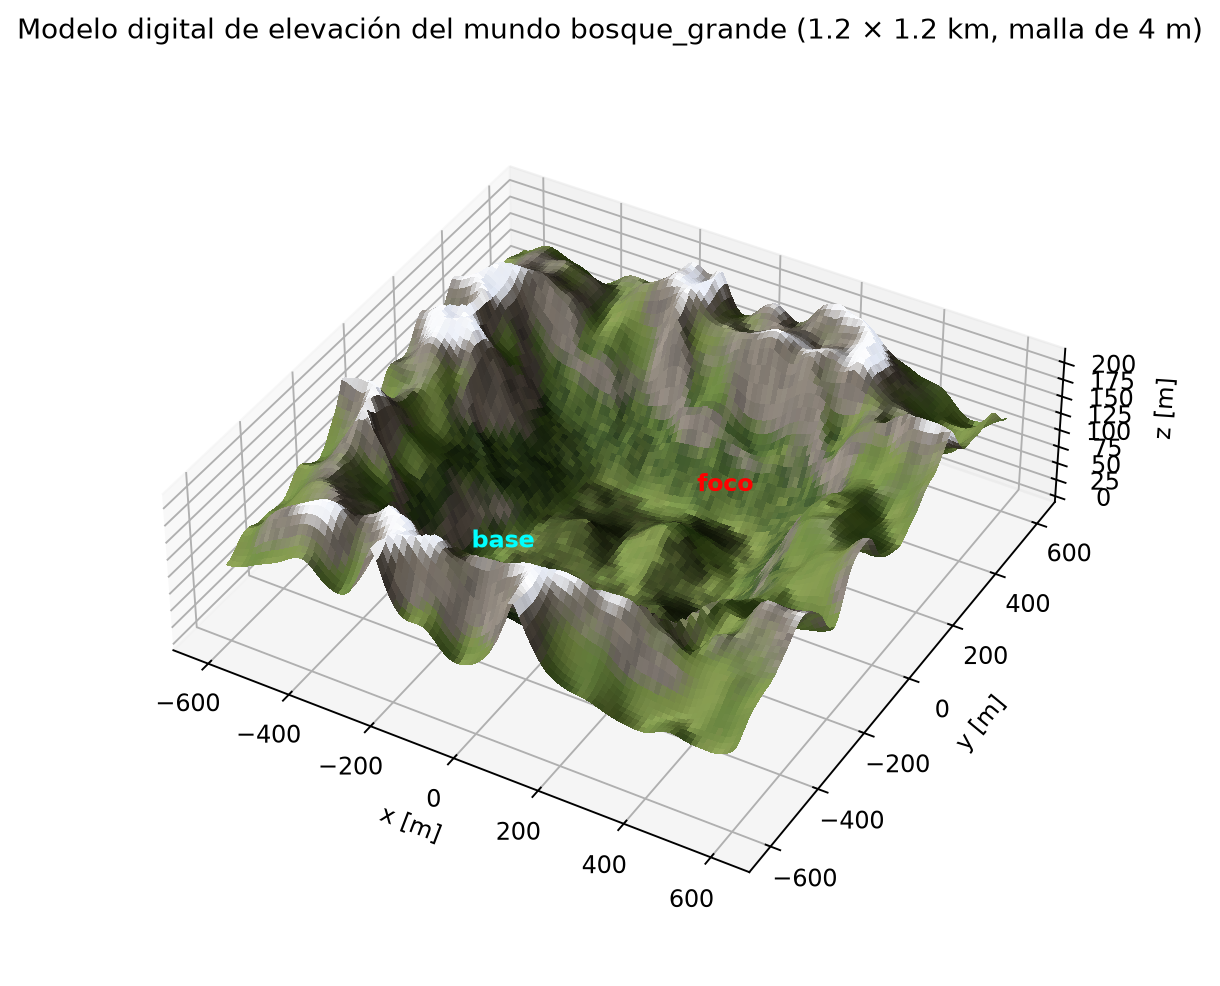
\includegraphics[width=0.9\textwidth]{dem_3d.png}
\caption{Modelo digital de elevación con la textura generada.}
\label{fig:dem}
\end{figure}

\begin{leccion}
La primera versión hacía que Gazebo se cayera con \emph{segfault} en
\cod{OdeMesh::fillArrays} en cuanto el dron tocaba algo. La causa: las mallas OBJ de colisión de las
rocas no traían normales. Se resolvió exportándolas con normales.
\end{leccion}

\subsection{El DEM y la clase \texttt{Terreno}}

\cod{altura.npz} guarda $x_0$, $y_0$, el paso y la matriz $h[i_y, i_x]$. \cod{cuadrirotor_sim/terreno.py}
interpola por triángulos (con la diagonal $(i_x,i_y)$--$(i_x{+}1,i_y{+}1)$, igual que la malla de
Gazebo) y ofrece:
\begin{itemize}
  \item \cod{altura(x, y)}: altura del suelo (vectorizada);
  \item \cod{maximo_en_tramo(a, b)}: punto más alto entre dos puntos (para seguir el relieve);
  \item \cod{cortar_rayo(o, d, alcance, desfase)}: dónde un rayo de la cámara toca el suelo.
\end{itemize}
Lo usan el planificador, la fauna (para caminar sobre el suelo, inclinados según la pendiente), el
\emph{launch} (para poner el dron y el foco sobre el terreno) y la captura de datos (para saber
qué tapa el relieve). Sin DEM, el suelo es el plano $z = 0$.

\subsection{Árboles en un solo modelo}

Para que 1700 árboles corran a tiempo real, todos van en un único modelo estático \cod{bosque}:
cada árbol es un \emph{visual} escalado (copa y corteza de la malla de OpenRobotics) y su
colisión es solo un cilindro en el tronco. Las rocas van igual en un modelo \cod{rocas}.

\subsection{Fauna}

Los modelos son CC0 de OpenGameArt: venado (crownjoshua), zorro y lobo (Quaternius).
\cod{scripts/preparar_fauna.py} los descarga, los gira a ``$z$ arriba y la cabeza hacia $+x$'',
los escala (venado 1.55~m, zorro 0.55~m, lobo 0.95~m), les pone colores por parte y los exporta a
\cod{models/fauna_*} (dinámicos, sin gravedad ni colisión). Se descartó un águila porque traía las
alas caídas.

El nodo \cod{fauna} (sin ROS, solo gz-transport) mueve a todos los animales con el servicio
\cod{/world/bosque_grande/set_pose_vector} a 10~Hz de tiempo simulado: alternan pausas (pastar,
olfatear) con caminatas a un punto al azar de su territorio; los lobos y zorros a veces trotan.

\begin{figure}[H]
\centering
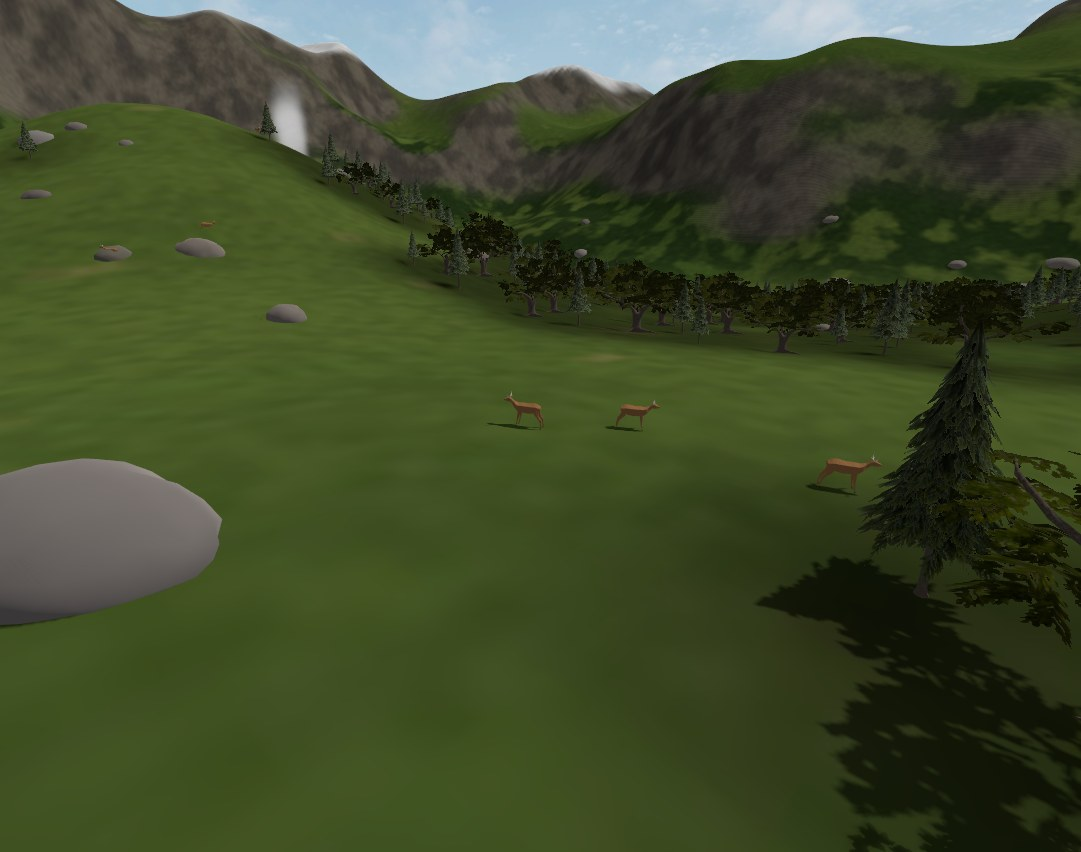
\includegraphics[width=0.49\textwidth]{gz_fauna.jpg}\hfill
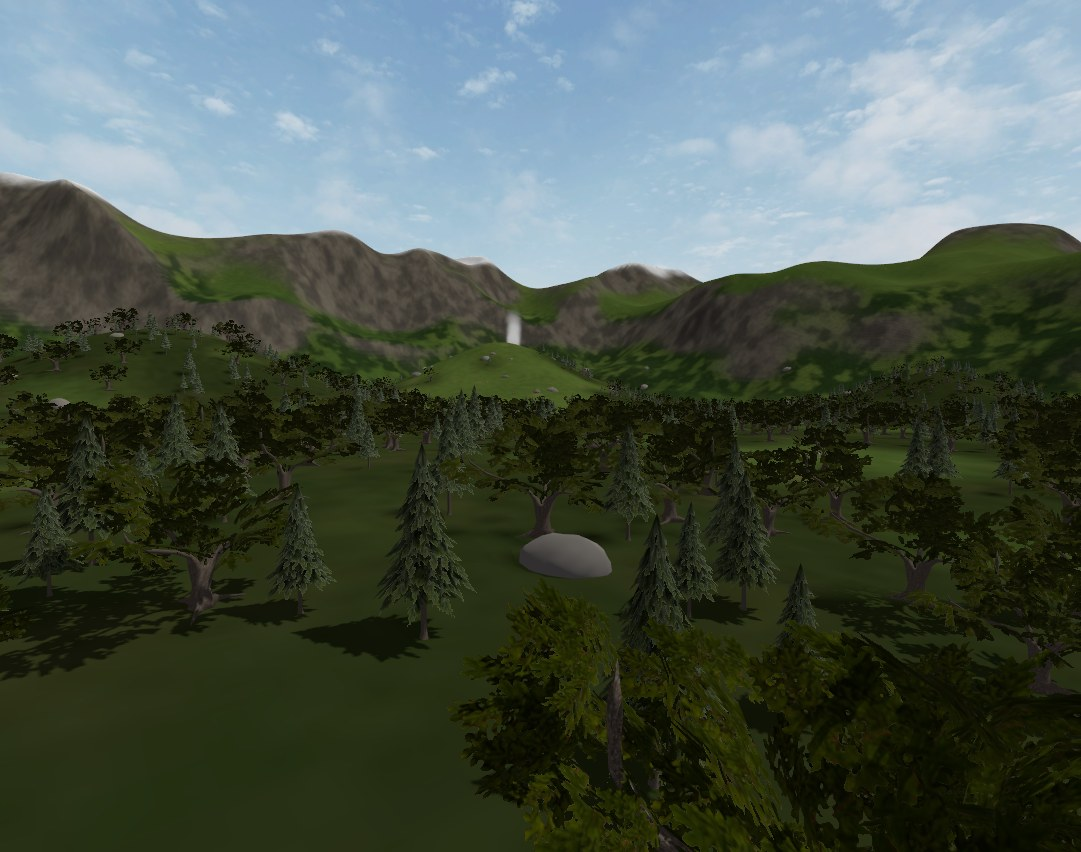
\includegraphics[width=0.49\textwidth]{gz_bosque_bajo.jpg}
\caption{Venados pastando en un claro (izquierda) y el bosque visto a baja altura (derecha).}
\end{figure}

\section{El incendio}

\cod{python3 scripts/generar_fuego.py} genera las texturas de las partículas y dos modelos:
\begin{itemize}
  \item \cod{foco_incendio}: siete emisores de llama (blanco amarillento $\rightarrow$ naranja
        $\rightarrow$ rojo $\rightarrow$ transparente), una columna de humo que crece y se aclara al
        subir, brasas, troncos carbonizados, suelo quemado y una luz naranja;
  \item \cod{columna_humo}: el penacho alto ($\approx$30~m, vida de 26~s) para el mundo grande.
\end{itemize}
Usan el sistema \cod{gz-sim-particle-emitter-system}; son solo visuales (no colisionan).

\begin{aviso}
Gazebo solo encuentra la imagen de rango de colores de las partículas
(\cod{<color_range_image>}) con una ruta absoluta. Por eso el \emph{launch} copia los dos modelos a
\cod{/tmp/cuadrirotor_sim_<uid>/modelos} con las rutas resueltas al arrancar.
\end{aviso}

\begin{figure}[H]
\centering
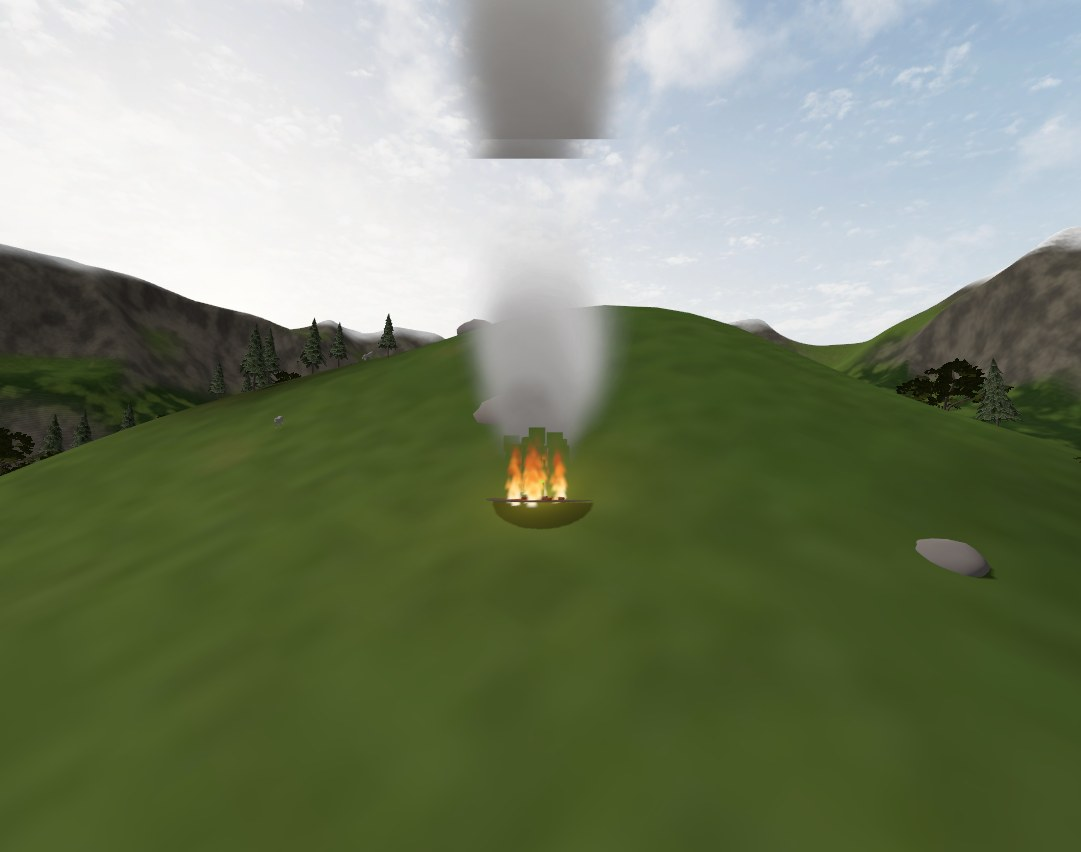
\includegraphics[width=0.62\textwidth]{gz_foco_cerca.jpg}
\caption{El foco de incendio en la ladera: llamas, claro quemado y columna de humo.}
\end{figure}

\section{Cómo arma el mundo el \emph{launch}}

Con \cod{mundo:=bosque_grande} el \emph{launch} (\cod{simulacion.launch.py}) escribe el SDF al
arrancar en \cod{/tmp/cuadrirotor_sim_<uid>/bosque_grande.sdf}, con el foco en
(\cod{foco_x}, \cod{foco_y}) sobre el terreno y el claro quemado alrededor
(\cod{cuadrirotor_sim/bosque_grande.py}). También:
\begin{itemize}
  \item pone el vehículo en la base, a la altura del DEM más 5~cm;
  \item lanza el nodo \cod{fauna};
  \item con GUI, arranca la cámara cerca de la base y a los 12~s llama a \cod{/gui/follow} y
        \cod{/gui/follow/offset} para que siga al dron;
  \item pasa al planificador \cod{config/mundo_bosque_grande.yaml} y la ruta del DEM.
\end{itemize}

El mundo está georreferenciado para que el GPS de Gazebo y el de ArduPilot coincidan con el aviso
del incendio (sección~\ref{sec:gps}):
\begin{lstlisting}[style=xml]
<spherical_coordinates>
  <surface_model>EARTH_WGS84</surface_model>
  <world_frame_orientation>ENU</world_frame_orientation>
  <latitude_deg>19.293</latitude_deg>
  <longitude_deg>-99.311</longitude_deg>
  <elevation>3000.0</elevation>
  <heading_deg>0</heading_deg>
</spherical_coordinates>
\end{lstlisting}

\begin{lstlisting}[style=bash]
# Foco en otro lugar del valle:
ros2 launch cuadrirotor_sim simulacion.launch.py vehiculo:=tarot650 mundo:=bosque_grande \
    controlador:=sta mision:=busqueda foco_x:=-150 foco_y:=60
\end{lstlisting}


\part{La autonomía: buscar el incendio sin piloto}
\chapter{Conceptos de autonomía}
\label{cap:conceptos-autonomia}

\begin{enpocas}
Qué significa que un dron sea autónomo, el ciclo percibir--decidir--actuar, las máquinas de estados,
cómo se planea recorrer toda una zona, cómo se ubica algo que se ve, qué es el GPS y cómo se pasa de
metros a latitud y longitud, qué es un LiDAR y cómo se esquivan obstáculos.
\end{enpocas}

\section{Percibir, decidir, actuar}

Un dron autónomo repite sin parar tres pasos:
\begin{figure}[H]
\centering
\begin{tikzpicture}[blq/.style={draw,rounded corners,fill=#1,minimum width=3.2cm,minimum height=1.1cm,align=center},
  fl/.style={-{Stealth[length=2.5mm]},very thick}]
  \node[blq=blue!12] (p) at (0,0) {\textbf{Percibir}\\cámara, YOLO, LiDAR,\\odometría};
  \node[blq=green!12] (d) at (5,0) {\textbf{Decidir}\\máquina de estados,\\ruta, estimación};
  \node[blq=red!10] (a) at (2.5,-2.6) {\textbf{Actuar}\\consigna $\rightarrow$\\controlador $\rightarrow$ motores};
  \draw[fl] (p) -- (d); \draw[fl] (d) -- (a); \draw[fl] (a) -- (p);
\end{tikzpicture}
\caption{El ciclo de la autonomía. En nuestra simulación se repite 50 veces por segundo.}
\end{figure}
En nuestro caso: \emph{percibir} es mirar con la cámara y el LiDAR; \emph{decidir} es elegir a dónde
ir (seguir la ruta, acercarse al humo, rodear un árbol); \emph{actuar} es mandar la consigna al
controlador, que mueve los motores.

\section{Máquinas de estados}

Un comportamiento complejo se organiza en \textbf{estados}: en cada momento el dron está en uno
(``patrullando'', ``acercándose al foco''...), hace lo que ese estado indica y cambia a otro cuando se
cumple una condición (``vi humo en tres imágenes seguidas'').

\begin{ejemplo}
Un semáforo es una máquina de estados: verde $\rightarrow$ (pasan 30~s) $\rightarrow$ amarillo
$\rightarrow$ (pasan 3~s) $\rightarrow$ rojo $\rightarrow$ ... Una lavadora también: llenar, lavar,
enjuagar, centrifugar.
\end{ejemplo}

La búsqueda del incendio tiene siete estados (figura~\ref{fig:estados}): despegue, patrulla,
hacia\_humo, aproximación, verificación, descenso y órbita. Es fácil de entender, de probar y de
explicar, y cuando algo falla el registro dice en qué estado estaba.

\section{Planear la cobertura: recorrer todo el bosque}

Si no sabemos dónde está el incendio, hay que mirar todo. Eso es un problema de \textbf{planificación
de cobertura}: encontrar una ruta que haga pasar la ``huella'' de la cámara por toda la zona. La
solución clásica es ir y venir en franjas paralelas, como al podar un jardín (en inglés,
\emph{boustrophedon}: ``como gira el buey al arar''). Lo que importa es la \textbf{separación} entre
franjas: tan grande como se pueda (ruta más corta) pero sin dejar huecos sin ver.

\begin{figure}[H]
\centering
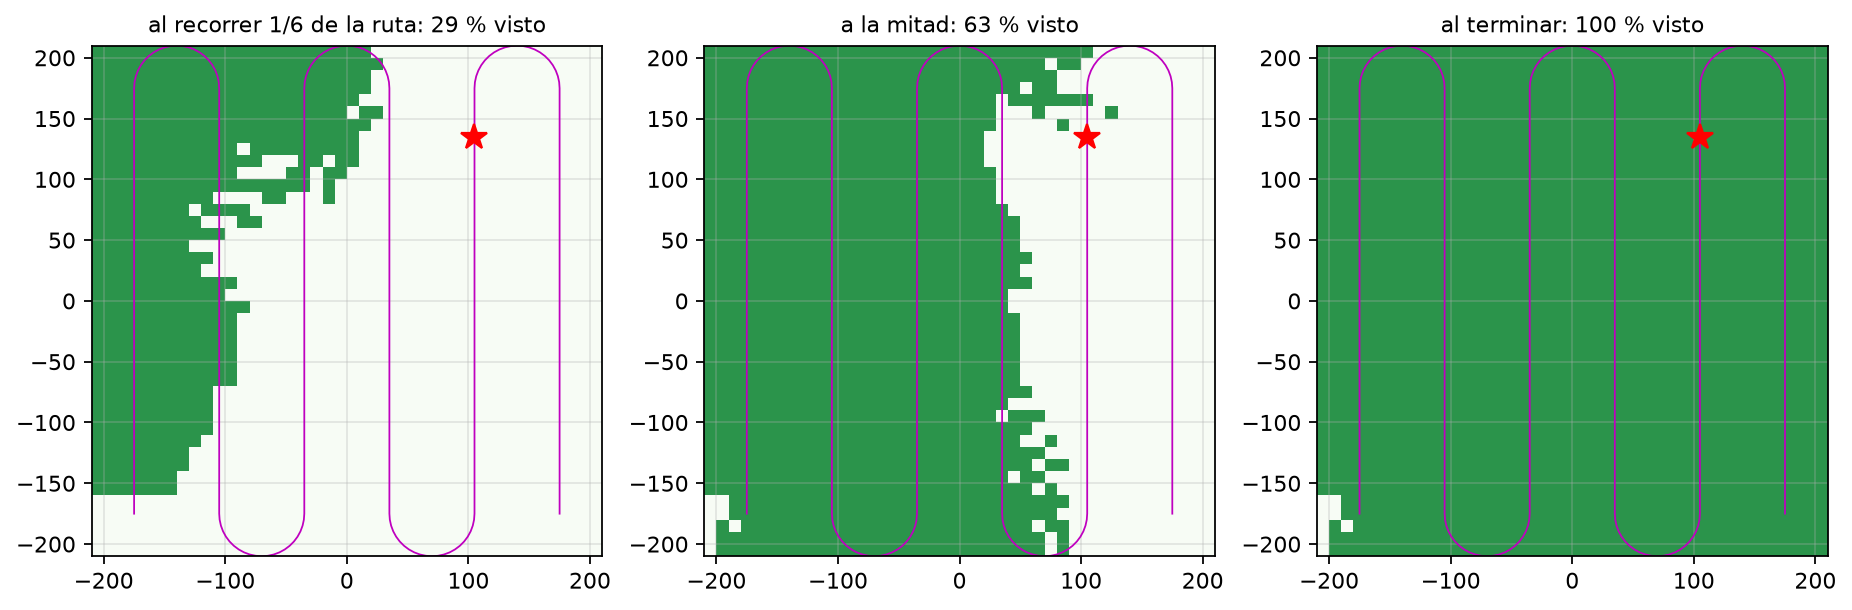
\includegraphics[width=\textwidth]{c_cobertura.png}
\caption{Simulación de qué tanto del bosque (celdas de 10~m) ha visto la cámara a lo largo de la
serpentina, a 30~m sobre el suelo y viendo hasta 150~m. La estrella roja es el incendio.}
\end{figure}

Durante el vuelo, el planificador lleva este mismo mapa (``cobertura'') y lo publica para verlo en
RViz.

\section{Ubicar lo que se ve}

Del capítulo~\ref{cap:imagen} sabemos que un píxel da una dirección. Para pasar a un punto del mapa hay dos caminos:

\textbf{Cortar el rayo con el terreno.} Si conocemos el relieve (un \textbf{modelo digital de
elevación}, DEM: una tabla con la altura del suelo cada 4~m), avanzamos por el rayo hasta que queda
por debajo del suelo. Así se estima la posición de las llamas.
\begin{figure}[H]
\centering
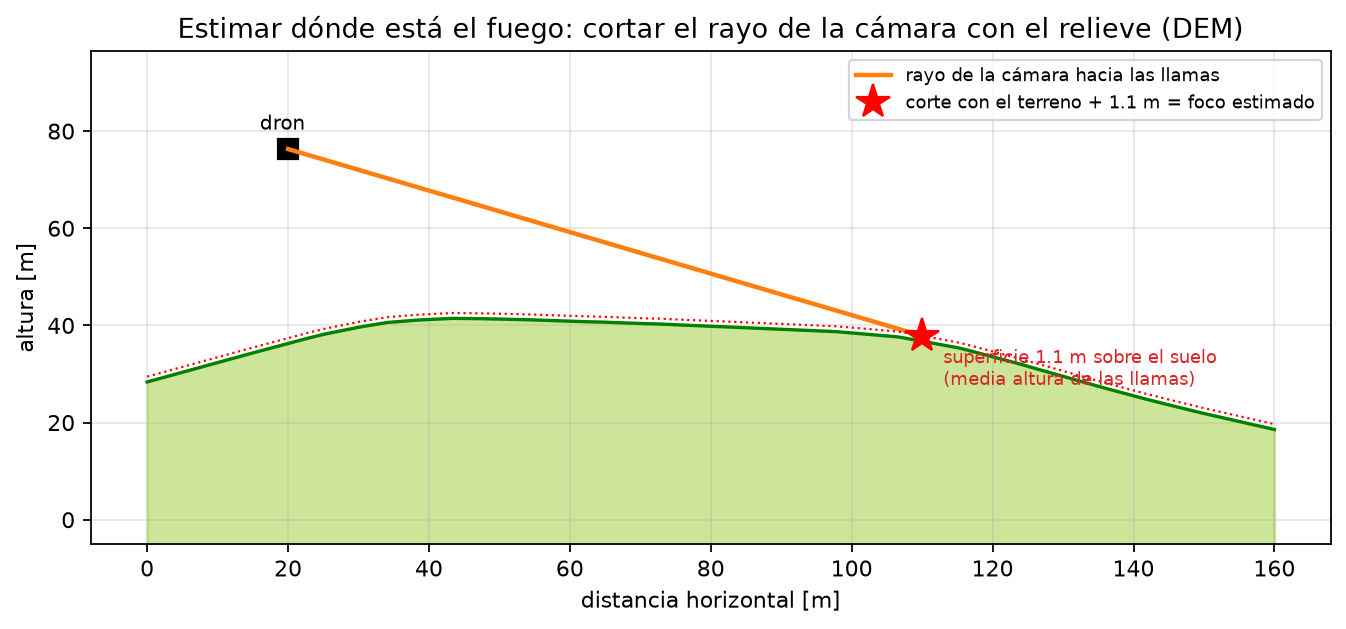
\includegraphics[width=0.9\textwidth]{c_rayo.png}
\caption{El rayo de la cámara hacia las llamas se corta con la superficie que está 1.1~m sobre el
relieve.}
\end{figure}

\textbf{Triangular.} El humo sube en columna vertical: verlo da la dirección hacia el foco pero no la
distancia. Con varias direcciones desde lugares distintos, el foco está donde se cruzan. Como las
mediciones tienen ruido, las rectas no se cruzan en un solo punto y se busca el más cercano a todas
(mínimos cuadrados).
\begin{figure}[H]
\centering
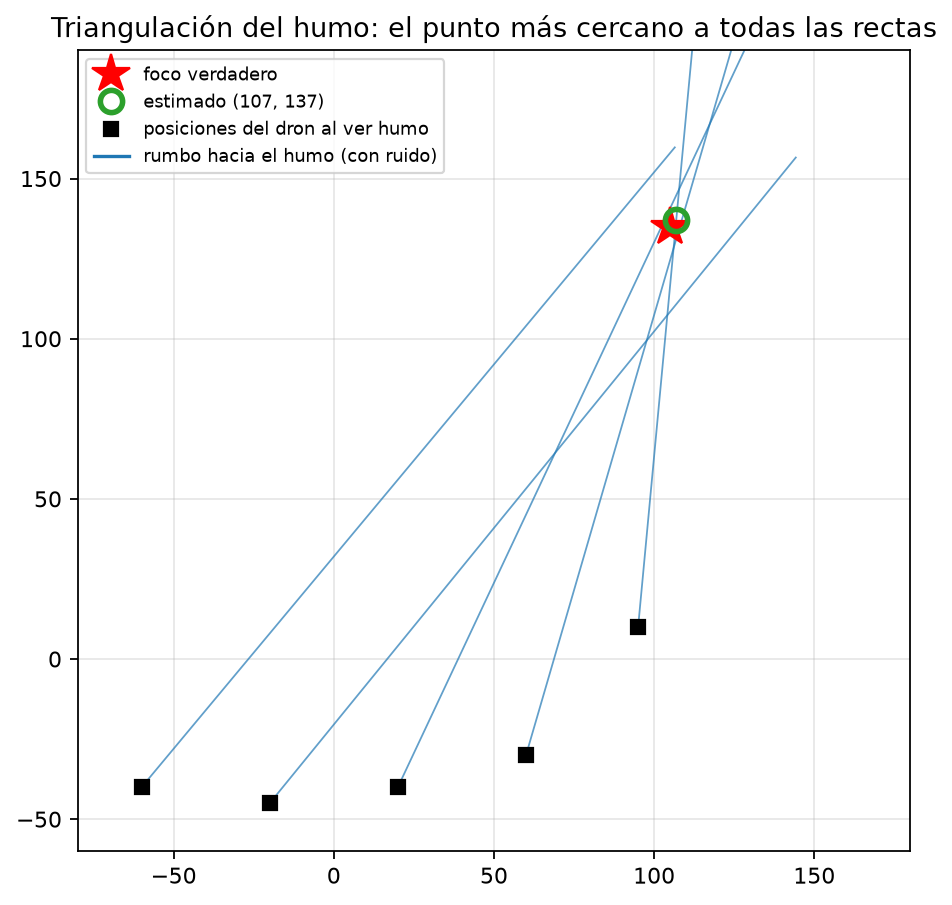
\includegraphics[width=0.7\textwidth]{c_triangulacion.png}
\caption{Triangulación del humo con cinco direcciones con ruido.}
\end{figure}

\begin{aviso}
La triangulación funciona mal si las direcciones son casi paralelas (todas vistas desde puntos
alineados en la misma dirección): un error pequeño en el ángulo mueve mucho el cruce. Por eso en la
simulación una estimación hecha solo con humo no basta para confirmar un incendio: el dron se acerca
hasta ver las llamas.
\end{aviso}

\section{GPS: de metros a latitud y longitud}

La simulación trabaja en metros sobre un plano (ENU), pero los bomberos necesitan
\textbf{coordenadas GPS}: latitud (cuánto al norte o sur del ecuador), longitud (cuánto al este u
oeste de Greenwich) y altitud. La Tierra no es una esfera sino un \textbf{elipsoide} un poco achatado;
el GPS usa el modelo \textbf{WGS84}.

\begin{figure}[H]
\centering
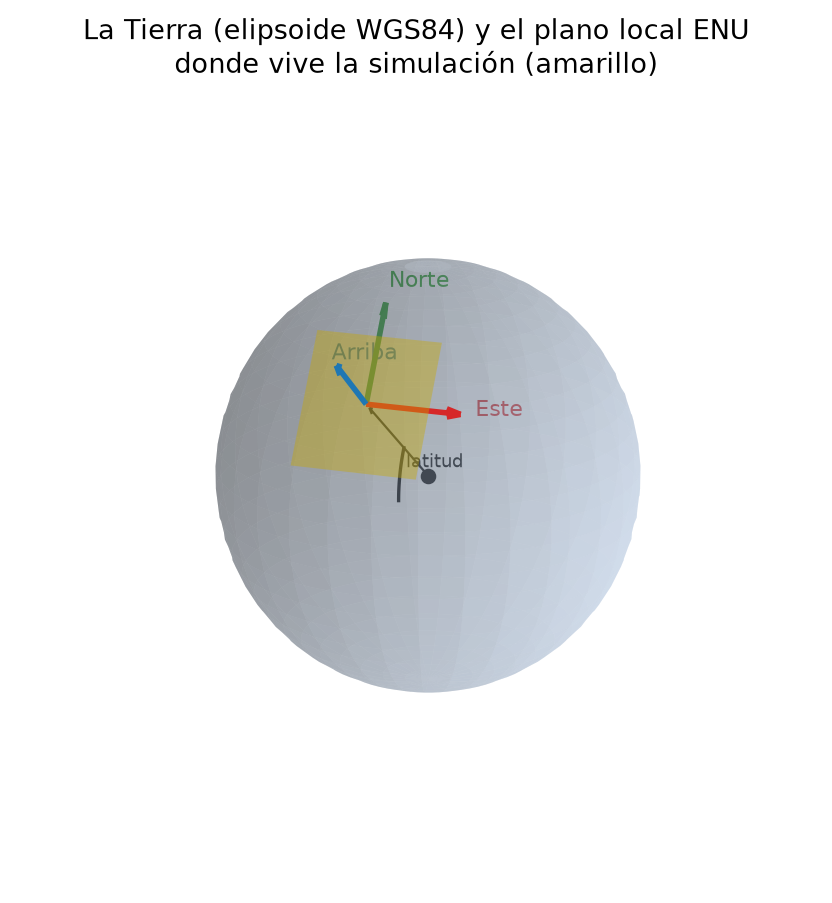
\includegraphics[width=0.6\textwidth]{c_tierra.png}
\caption{El plano local ENU de la simulación es tangente a la Tierra en el origen del mundo.}
\end{figure}

Para convertir se fija dónde está el origen del mundo (como supuesto, en el Parque Nacional Desierto
de los Leones, CDMX: 19.293° N, 99.311° O, 3000~m) y se hace la cuenta exacta: ENU $\rightarrow$
coordenadas cartesianas centradas en la Tierra (ECEF) $\rightarrow$ latitud, longitud y altitud
(sección~\ref{sec:gps}).

\begin{tecnico}
A esta latitud, un grado de latitud mide unos 110.8~km y uno de longitud unos 105.1~km. Por eso un
error de $10^{-6}$ grados en las coordenadas equivale a unos 10~cm: con seis decimales basta.
\end{tecnico}

\section{LiDAR: medir distancias con luz}

Un \textbf{LiDAR} lanza pulsos láser en muchas direcciones y mide cuánto tardan en regresar; con eso
calcula la distancia al primer obstáculo en cada dirección. El resultado es una \textbf{nube de
puntos}. El del dron simulado lanza 120 rayos alrededor por 16 alturas distintas, 10 veces por
segundo, hasta 30~m.

\begin{figure}[H]
\centering
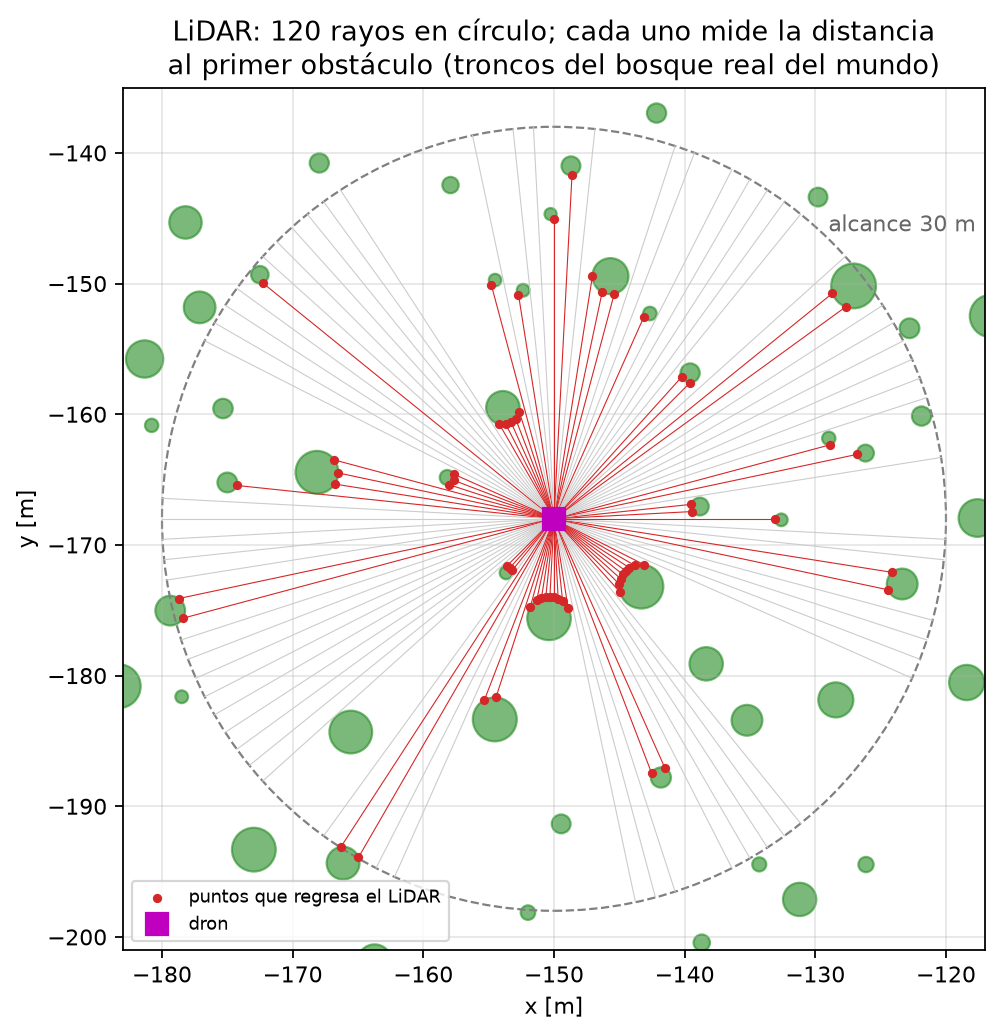
\includegraphics[width=0.6\textwidth]{c_lidar.png}
\caption{Una capa del LiDAR en el bosque del mundo grande: los rayos rojos tocan un tronco, los grises
no encuentran nada en 30~m.}
\end{figure}

A diferencia de la cámara, el LiDAR sí da distancias, pero no sabe ``qué'' es cada punto. Se
complementan: la cámara para reconocer el fuego, el LiDAR para no chocar.

\section{Evitar obstáculos}

Hay dos grandes familias de métodos:
\begin{description}
  \item[Planificación global:] con un mapa completo, se calcula de antemano una ruta sin choques
        (algoritmos como A* o RRT).
  \item[Evasión reactiva:] con lo que se ve en ese momento, se corrige el rumbo sobre la marcha.
        Es lo que hacemos: no tenemos un mapa de los árboles, solo lo que ve el LiDAR.
\end{description}
Nuestro método es del tipo \textbf{VFH} (\emph{vector field histogram}): se divide el círculo de
direcciones alrededor del dron en 72 sectores, se marcan los que están bloqueados por algún obstáculo
cercano y se elige el sector libre más parecido a la dirección a la que queremos ir.

\begin{figure}[H]
\centering
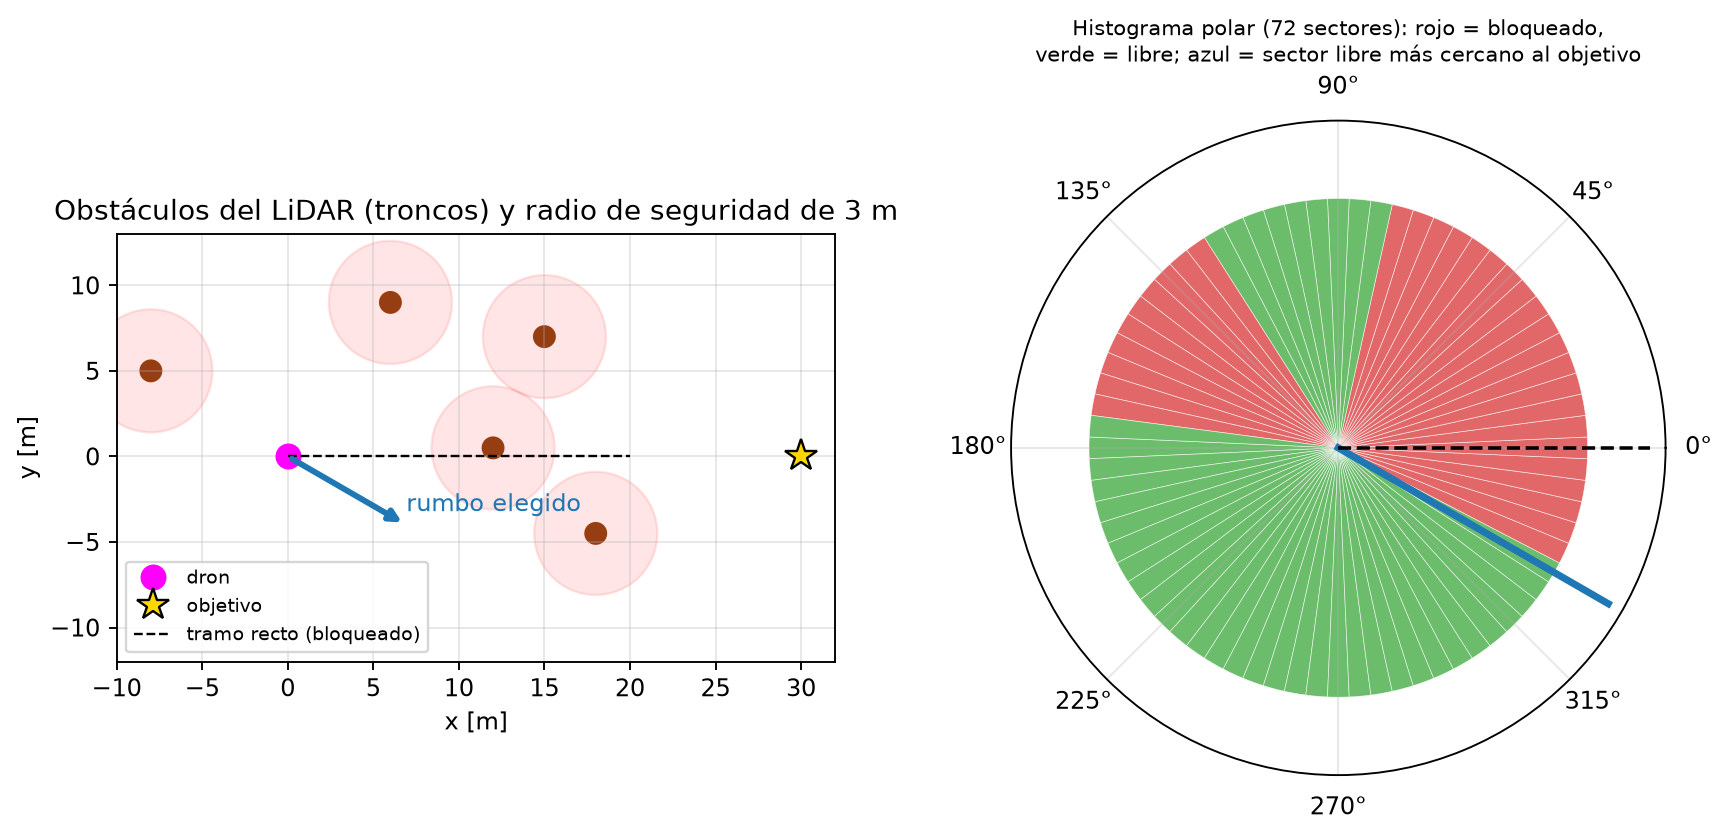
\includegraphics[width=\textwidth]{vfh.png}
\caption{Evasión con histograma polar.}
\end{figure}

Para las montañas no hace falta el LiDAR: el relieve se conoce (el DEM), así que el dron sube antes de
llegar a una ladera. El capítulo siguiente cuenta cómo se juntaron todas estas piezas.

\chapter{La búsqueda del incendio, pieza por pieza}

\begin{enpocas}
Cómo quedó programado el planificador \cod{busqueda_incendio}: la máquina de estados, la ruta en serpentina, el seguimiento del relieve, la estimación y confirmación del foco, el aviso GPS y la evasión de obstáculos, con sus fórmulas y parámetros.
\end{enpocas}
\label{cap:autonomia}

\begin{lstlisting}[style=bash]
ros2 launch cuadrirotor_sim simulacion.launch.py vehiculo:=tarot650 mundo:=bosque_grande \
    controlador:=sta mision:=busqueda
\end{lstlisting}

Con \cod{mision:=busqueda} el \emph{launch} agrega el detector y el planificador
\cod{busqueda_incendio}, y pone al controlador en modo \cod{externa}: deja de generar su propia
referencia y sigue la consigna que publica el planificador en \cod{/cuadrirotor/consigna}
(\cod{trajectory_msgs/MultiDOFJointTrajectoryPoint}: posición, velocidad, aceleración y guiñada).
El planificador corre a 50~Hz y limita la velocidad (5~m/s horizontal, 3~m/s vertical) y la
aceleración (1.5~m/s$^2$) de la consigna.

\section{Máquina de estados}

\begin{figure}[H]
\centering
\begin{tikzpicture}[
  est/.style={draw,rounded corners,fill=#1,minimum width=2.6cm,minimum height=0.9cm,align=center,font=\small},
  est/.default=green!10,
  fl/.style={-{Stealth[length=2.2mm]},thick},
  et/.style={font=\scriptsize,align=center,fill=white,inner sep=1pt}]
  \node[est=black!5] (des) at (0,0) {despegue};
  \node[est] (pat) at (0,-2.8) {patrulla};
  \node[est] (hum) at (7,-2.8) {hacia\_humo};
  \node[est] (apr) at (0,-6.2) {aproximacion};
  \node[est=yellow!20] (ver) at (7,-6.2) {verificacion};
  \node[est] (bajo) at (0,-8.9) {descenso};
  \node[est=red!12] (orb) at (0,-11.4) {orbita\\+ aviso GPS};
  \draw[fl] (des) -- node[et,left]{altura de búsqueda\\alcanzada} (pat);
  \draw[fl] (pat) to[bend left=18] node[et,above]{humo en 3 imágenes seguidas} (hum);
  \draw[fl] (hum) to[bend left=18] node[et,below]{humo perdido 6 s} (pat);
  \draw[fl] (pat) -- node[et,left]{hay estimación\\del foco} (apr);
  \draw[fl] (hum) -- node[et,pos=0.62,above,sloped]{hay estimación} (apr);
  \draw[fl] (apr) to[bend right=18] node[et,below]{en el anillo y solo con humo} (ver);
  \draw[fl] (ver) to[bend right=18] node[et,above,pos=0.7]{ve las llamas} (apr);
  \draw[fl] (ver.east) -- ++(1.3,0) |- node[et,pos=0.25,right]{2 min sin\\ver llamas} ($(pat.north east)+(0,0.8)$) -- (pat.north east);
  \draw[fl] (apr) -- node[et,left]{en el anillo,\\estimación con llamas} (bajo);
  \draw[fl] (bajo) -- node[et,left]{altura de órbita\\y mirando al foco} (orb);
\end{tikzpicture}
\caption{Estados de \cod{busqueda_incendio}. En \emph{patrulla}, al terminar la ruta sin ver el
incendio, el dron la recorre de regreso y sigue vigilando.}
\label{fig:estados}
\end{figure}

\section{Ruta de barrido en serpentina}

La zona del bosque es el rectángulo $[-210,210]\times[-210,210]$~m. La ruta (\cod{cobertura.py},
\cod{ruta_serpentina}) avanza \textbf{hacia el frente del dron}: en el eje de la zona más parecido a
su rumbo al despegar (en la base mira a $+x$). Los barridos son perpendiculares al avance, de lado a
lado del bosque, separados $p\approx70$~m y a $p/2$ de los bordes; cada uno se une con el siguiente
por un semicírculo de radio $r = p/2 = 35$~m. Con $f$ la coordenada de avance, $l$ la lateral,
$\sigma=\pm1$ el lado de la vuelta y $\phi\in[0,\pi]$:
\begin{equation}
(f, l) = \big(f_k + r(1-\cos\phi),\ l_{fin} + \sigma r\sin\phi\big).
\end{equation}
La ruta se muestrea cada 5~m (2.6~km, $\approx$9~min a 5~m/s) y el dron persigue un punto 10~m
adelante sobre ella (\cod{anticipo_ruta}), así que no frena en las vueltas: a 5~m/s la vuelta pide
$v^2/r = 0.7$~m/s$^2$. La versión anterior (\cod{patron: franjas}) recorría franjas este-oeste con
vueltas en ángulo recto, deteniéndose en cada vértice.

\begin{figure}[H]
\centering
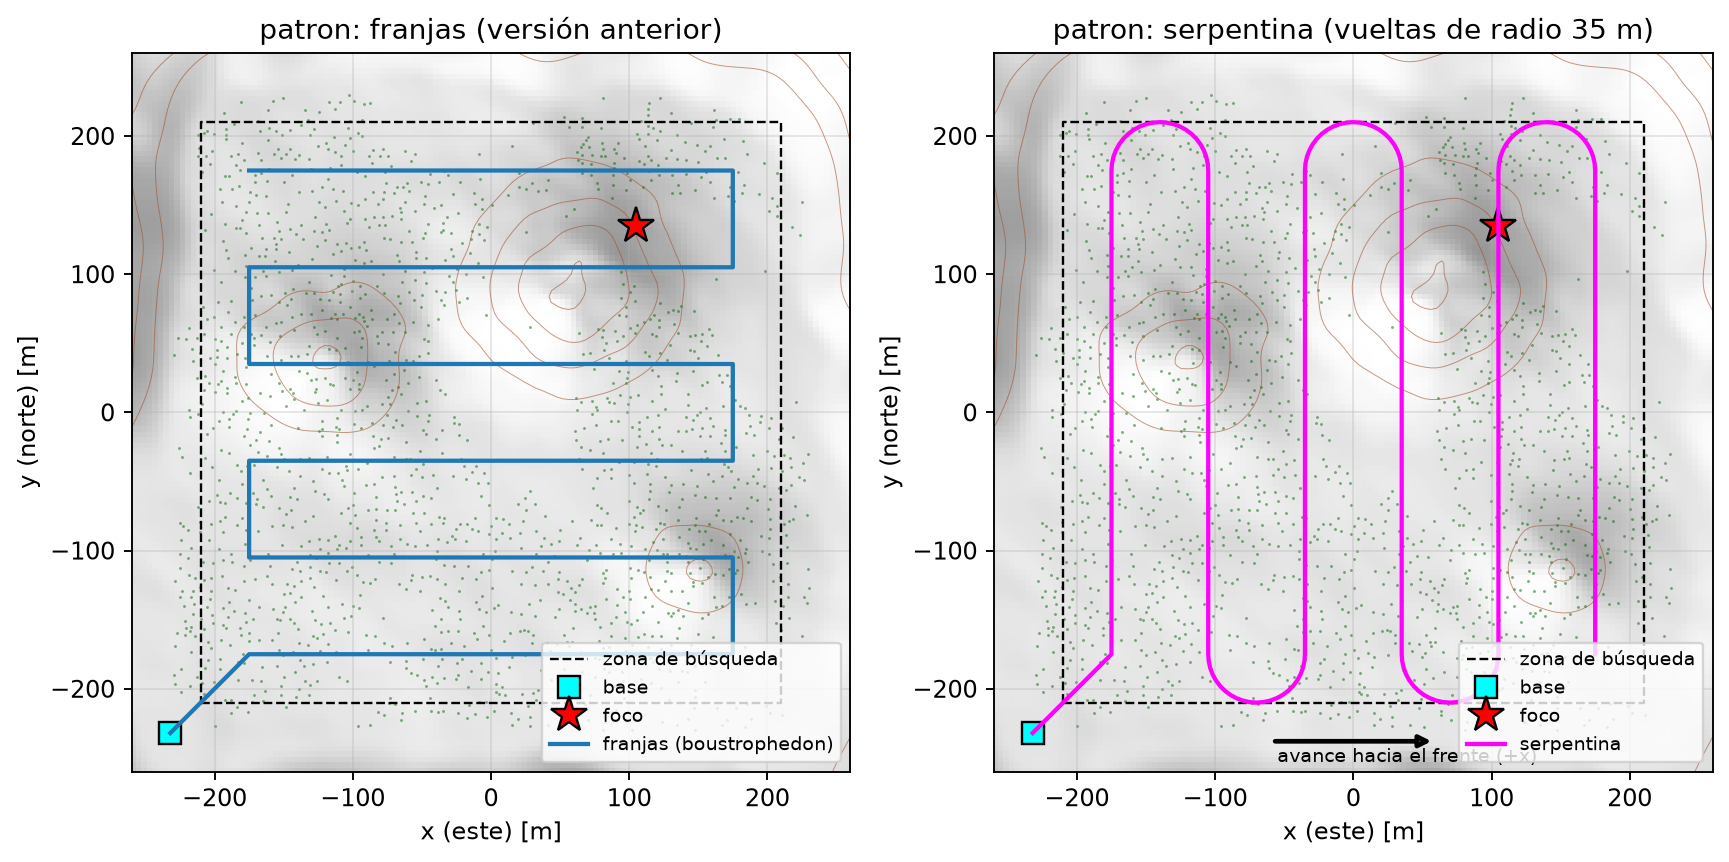
\includegraphics[width=\textwidth]{rutas.png}
\caption{Rutas sobre el relieve (curvas de nivel cada 10~m) y los árboles (puntos verdes).}
\label{fig:rutas}
\end{figure}

\section{Seguimiento del relieve}

Las alturas son \emph{sobre el suelo}. La altura de la consigna es
\begin{equation}
z = \max_{q\,\in\,[c,\ c + L\hat u]} h(q) + h_{busq},\qquad L = 50\ \text{m},\ h_{busq} = 30\ \text{m},
\end{equation}
el punto más alto del terreno entre la consigna $c$ y 50~m adelante (\cod{anticipacion}), más un
margen de 5~m a los lados. Así el dron empieza a subir antes de llegar a un cerro. El planificador
conoce el relieve (como un dron real con un mapa de elevación), pero no dónde está el incendio.

\section{Mapa de cobertura}

Cada 0.5~s se proyecta una rejilla de $24\times18$ rayos de la cámara sobre el relieve (hasta
150~m) y se marcan las celdas de $10\times10$~m que ya se vieron. Se publica el porcentaje en
\cod{/cuadrirotor/busqueda/cobertura} y el mapa en \cod{/cuadrirotor/busqueda/mapa_cobertura}
(\cod{nav_msgs/OccupancyGrid}, 0 = vista), junto con la ruta en \cod{/cuadrirotor/busqueda/ruta}.
Se ven en RViz con el marco \cod{world}.

\section{Estimación de la posición del foco}

Cada detección se empareja con la pose del dron en el instante de la imagen. El rayo de la cámara
por el centro de la caja $(u,v)$ es
\begin{equation}
d = R\,R_c\begin{bmatrix}1\\ -(u - W/2)/f\\ -(v - H/2)/f\end{bmatrix},\qquad
f = \frac{W/2}{\tan(\text{HFOV}/2)},
\end{equation}
con $R_c$ la inclinación de 30° de la cámara.

\textbf{Con llamas.} El rayo se corta con la superficie 1.1~m sobre el suelo (media altura de las
llamas) con \cod{Terreno.cortar_rayo}, solo si el corte queda a menos de 100~m
(\cod{alcance_llamas}). La estimación es la mediana de los últimos 15 cortes (con al menos 5).

\textbf{Con humo.} La columna es vertical sobre el foco, así que cada detección da solo un rumbo
$\hat n_i$ desde la posición $c_i$ de la cámara. Con rumbos desde puntos distintos (dispersión de
más de 0.25~rad) se busca el punto más cercano a todas las rectas por mínimos cuadrados:
\begin{equation}
\hat x = \Big(\sum_i P_i\Big)^{-1}\sum_i P_i\,c_i,\qquad P_i = I - \hat n_i\hat n_i^\top .
\end{equation}

\begin{leccion}
Antes del límite \cod{alcance_llamas}, con el foco en $(-150,60)$ la primera estimación caía en
$(-137,110)$: de lejos el rayo roza el suelo y un error pequeño en la caja da decenas de metros.
\end{leccion}

\section{Verificación: solo con llamas se confirma}

Si al llegar al anillo de órbita la estimación sigue saliendo solo del humo, el dron entra en
\emph{verificacion}: rodea el punto estimado a 35~m y a la altura de búsqueda, mirándolo, hasta ver
las llamas; con ellas vuelve a \emph{aproximacion} con la estimación corregida. Si no las ve en
2~min, descarta la estimación y sigue la patrulla. Solo con llamas baja a orbitar y avisa.

\section{Órbita}

Radio 14~m, $\omega = 0.12$~rad/s (con rampa de 4~s), cámara hacia el foco y altura
\begin{equation}
z_{orb} = \max\big(h(\text{foco}) + 18\ \text{m},\ \max_{\text{anillo}} h + 14\ \text{m}\big),
\end{equation}
por encima de las copas (los árboles miden hasta 8.2~m). Si el LiDAR ve algo más alto bajo el
anillo, sube (a lo más 1~m/s).

\begin{figure}[H]
\centering
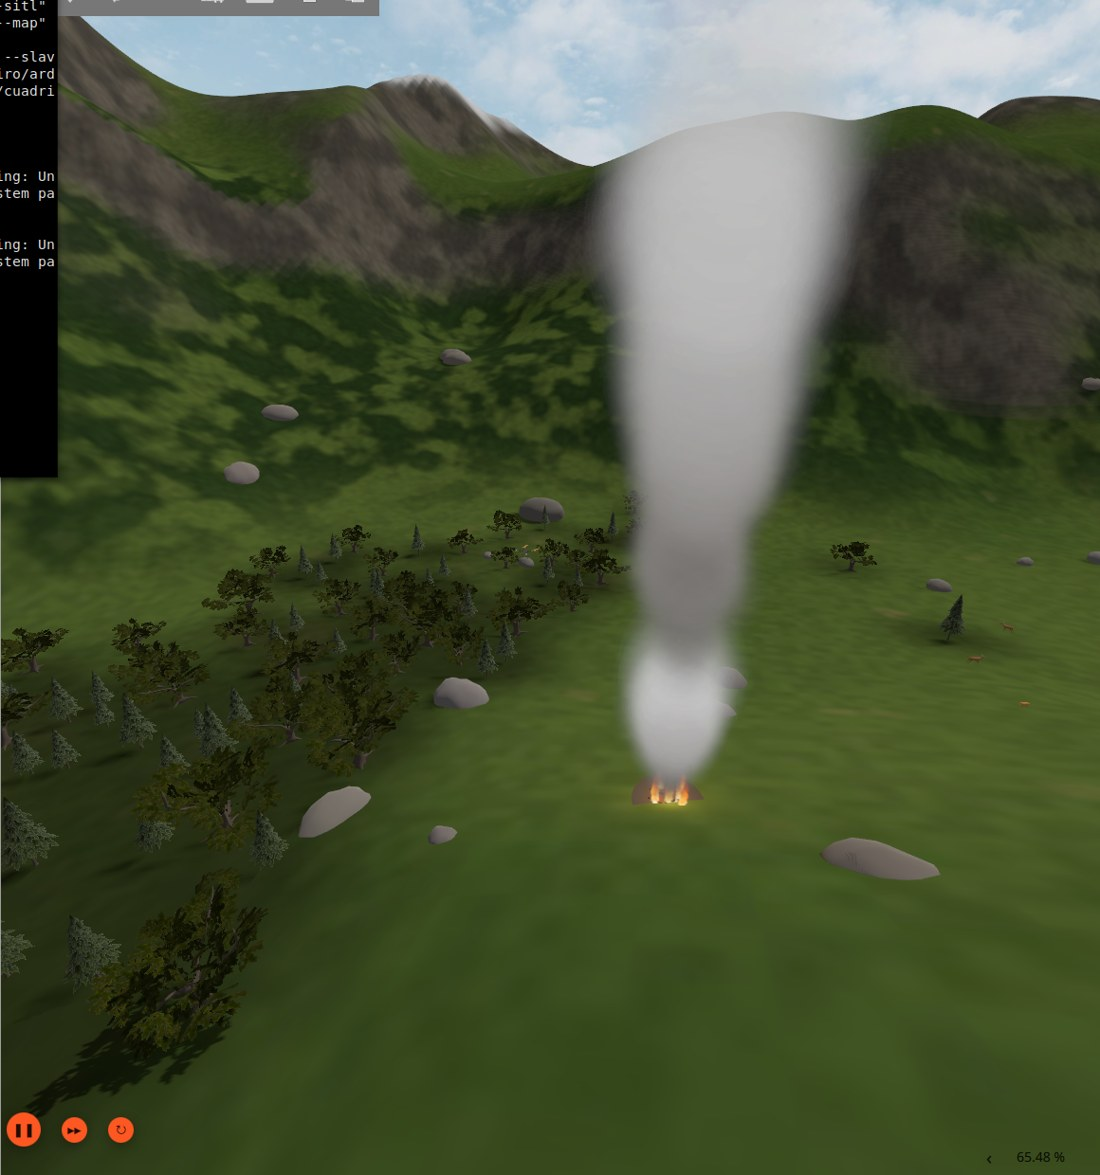
\includegraphics[width=0.62\textwidth]{gazebo_humo.jpg}
\caption{El dron llegando al foco: la cámara de Gazebo sigue al dron desde atrás.}
\end{figure}

\section{Aviso con las coordenadas GPS}
\label{sec:gps}

Al empezar la órbita (foco confirmado y visto de cerca) el planificador publica una sola vez:
\begin{itemize}
  \item \cod{/cuadrirotor/incendio/gps}: \cod{sensor_msgs/NavSatFix} con latitud, longitud, altitud
        y la dispersión de los cortes de las llamas como incertidumbre;
  \item \cod{/cuadrirotor/incendio/alerta}: el aviso de texto.
\end{itemize}
Los dos con QoS \emph{transient local}: quien se suscriba después también lo recibe. Además lo
escribe en la terminal y agrega una línea a \cod{~/incendios_detectados.csv}:

\begin{lstlisting}
INCENDIO CONFIRMADO 2026-10-23 04:26:47
  GPS: 19.294219, -99.310000  (19°17'39.2"N 99°18'36.0"W)
  Altitud del suelo: 3019 m   incertidumbre: ±1.0 m
  Mapa: https://www.google.com/maps?q=19.294219,-99.310000
  Local: (105.1, 135.0) m
\end{lstlisting}

Para recibirlo desde otra terminal: \cod{ros2 topic echo /cuadrirotor/incendio/alerta}.

\textbf{Conversión ENU $\rightarrow$ WGS84} (\cod{geo.py}). El origen del mundo se puso, como
supuesto, en el Parque Nacional Desierto de los Leones (CDMX), un bosque de oyamel con incendios
casi cada temporada seca: $\varphi_0 = 19.2930^\circ$, $\lambda_0 = -99.3110^\circ$, $h_0 = 3000$~m (el
relieve del mundo no es el real; parámetro \cod{origen_gps} para cambiarlo). La conversión es
exacta sobre el elipsoide WGS84 ($a = 6378137$~m, $e^2 = 6.69437999014\times10^{-3}$). El origen
pasa a ECEF con $N(\varphi) = a/\sqrt{1-e^2\sin^2\varphi}$:
\begin{equation}
X_0 = (N+h_0)\cos\varphi_0\cos\lambda_0,\quad
Y_0 = (N+h_0)\cos\varphi_0\sin\lambda_0,\quad
Z_0 = (N(1-e^2)+h_0)\sin\varphi_0 ,
\end{equation}
el punto $(x,y,z)$ en ENU se rota al ECEF,
\begin{equation}
\begin{bmatrix}X\\Y\\Z\end{bmatrix} = \begin{bmatrix}X_0\\Y_0\\Z_0\end{bmatrix} +
\begin{bmatrix}
-\sin\lambda_0 & -\sin\varphi_0\cos\lambda_0 & \cos\varphi_0\cos\lambda_0\\
\cos\lambda_0 & -\sin\varphi_0\sin\lambda_0 & \cos\varphi_0\sin\lambda_0\\
0 & \cos\varphi_0 & \sin\varphi_0
\end{bmatrix}
\begin{bmatrix}x\\y\\z\end{bmatrix},
\end{equation}
y se regresa a geodésicas iterando $\varphi \leftarrow \operatorname{atan2}\big(Z,\ p(1 - e^2N/(N+h))\big)$,
$h = p/\cos\varphi - N$, con $p = \sqrt{X^2+Y^2}$ y $\lambda = \operatorname{atan2}(Y, X)$.

\section{Evasión de obstáculos}

Se pidió que el dron no choque con las montañas ni con los árboles. Toda consigna, salvo la de la
órbita, pasa por dos filtros (\cod{_seguro} del planificador y \cod{cuadrirotor_sim/evasion.py}):

\subsection{Relieve: primero subir}

Con \cod{altura_seguridad} $> 0$ (10~m en el mundo grande), si la consigna está a menos de esa
altura sobre el punto más alto del terreno en los próximos 25~m, el objetivo horizontal se congela
en la posición actual y solo se sube. El dron nunca avanza ``hacia'' una ladera más rápido de lo
que puede subir.

\subsection{Árboles, rocas y animales: LiDAR y histograma polar}

\begin{enumerate}
  \item \textbf{Memoria de obstáculos.} Cada nube del LiDAR pasa al marco del mundo con la pose del
        dron en ese instante, $p_w = p + R\,(q + r_{lidar})$. Se quitan los puntos a menos de 1.5~m
        del DEM (son el suelo) y el resto se guarda en vóxeles de 1~m, olvidando lo que queda a más
        de 60~m del dron. Se publican en \cod{/cuadrirotor/evasion/obstaculos}.
  \item \textbf{¿Está libre el camino?} Se toman los puntos a la altura del dron ($\pm3$~m) y a menos
        de 20~m. Si ninguno queda a menos de $r = 3$~m del tramo recto hacia el objetivo, la consigna
        no se toca.
  \item \textbf{Histograma polar} (como VFH). Si el tramo está bloqueado, se dividen las direcciones
        en 72 sectores de 5°. Un punto a distancia $d$ y ángulo $\theta$ bloquea los sectores dentro de
        $\theta\pm\big(\arcsin(r/d) + 2.5^\circ\big)$, es decir, todo rumbo que pasaría a menos de $r$ de él.
  \item \textbf{Elección.} Se toma el sector libre que minimiza
        $|\theta - \theta_{obj}| + 0.3\,|\theta - \theta_{prev}|$ (el segundo término evita
        oscilar) y el objetivo pasa a ser un punto a 8~m en esa dirección. Si todos están bloqueados,
        el objetivo es subir 4~m.
  \item \textbf{Histéresis.} Mientras está desviado, solo vuelve al tramo recto cuando queda libre con
        $1.4\,r$.
  \item \textbf{Al bajar} no entra a menos de $r$ de lo más alto que tenga debajo.
\end{enumerate}

\begin{figure}[H]
\centering
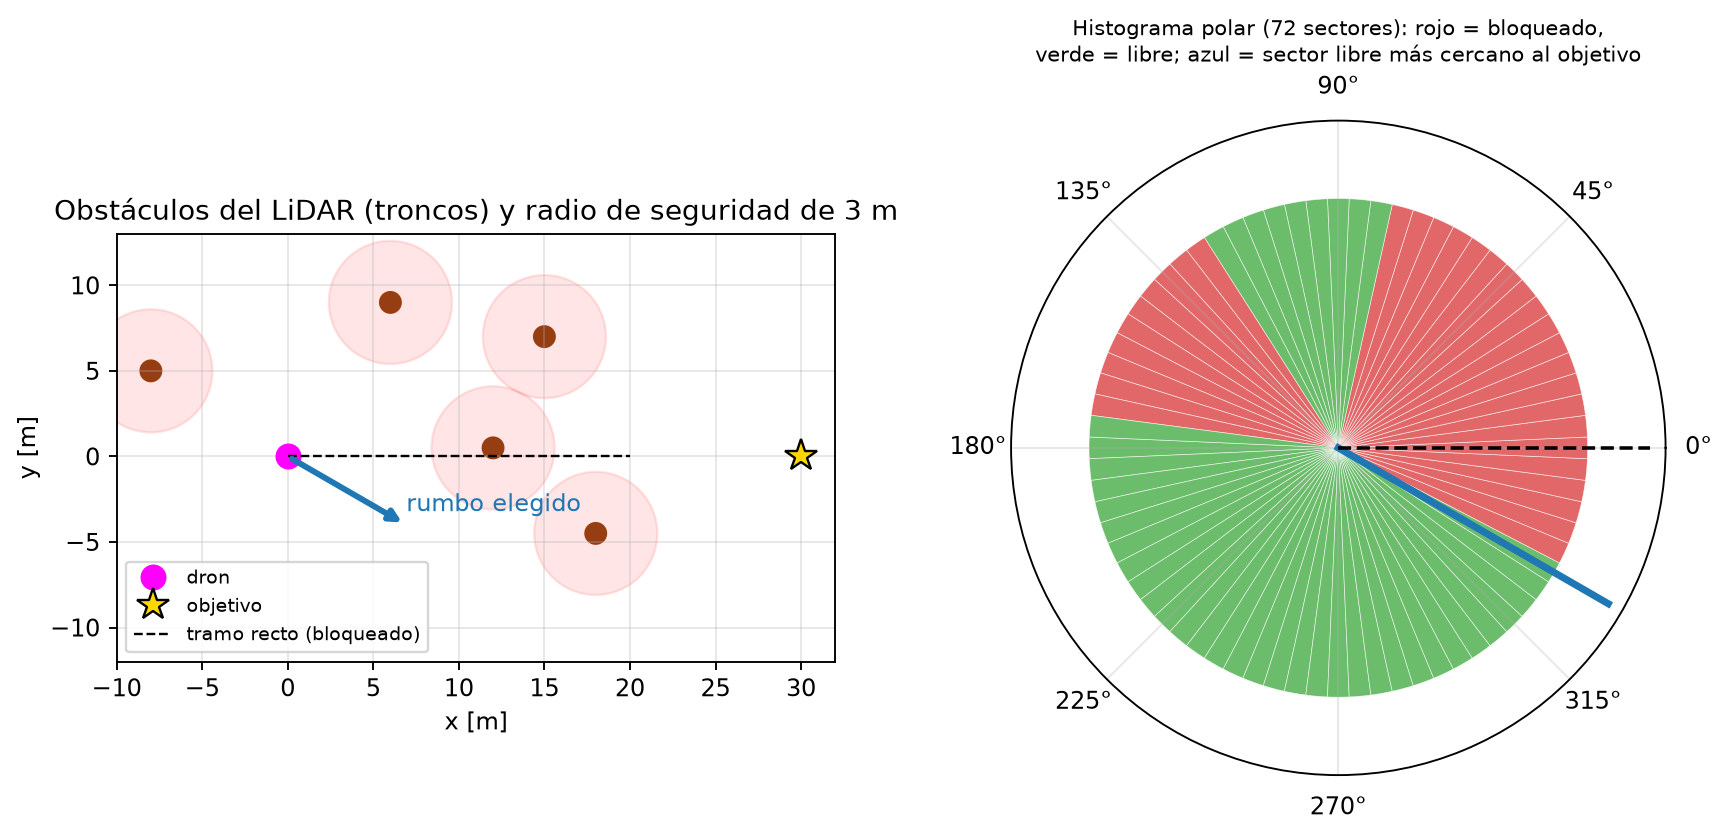
\includegraphics[width=\textwidth]{vfh.png}
\caption{Ejemplo del algoritmo: el tramo recto al objetivo choca con un tronco; el histograma polar
marca los sectores bloqueados y el dron toma el libre más cercano al rumbo del objetivo.}
\label{fig:vfh}
\end{figure}

El núcleo de \cod{Evasion.corregir}:
\begin{lstlisting}[style=py]
r = np.linalg.norm(Q, axis=1)                      # puntos (xy relativos) a la altura del dron
ang = np.arctan2(Q[:, 1], Q[:, 0])
ancho = np.arcsin(np.minimum(1.0, self.radio / np.maximum(r, 1e-3))) + self.medio_sector
bloq = (np.abs(envolver(self.th[:, None] - ang[None, :])) < ancho[None, :]).any(axis=1)
if bloq.all():                                     # sin salida: sube
    return np.array([c[0], c[1], c[2] + self.subida])
costo = np.abs(envolver(self.th - rumbo_g))
if self.rumbo_previo is not None:
    costo = costo + 0.3 * np.abs(envolver(self.th - self.rumbo_previo))
costo[bloq] = np.inf
rumbo = float(self.th[np.argmin(costo)])
\end{lstlisting}

\textbf{Prueba.} Para forzar la evasión se puso \cod{altura_busqueda: 5} (5~m sobre el suelo, entre
árboles de hasta 8.2~m). En 540~m de patrulla el dron se desvió 12 veces y \textbf{ninguna muestra
quedó dentro de una copa}: la holgura mínima a la copa más cercana fue de 0.5~m, a unos 2.2~m/s. A
los 30~m de la búsqueda normal los árboles no estorban y la evasión casi nunca actúa.

\begin{figure}[H]
\centering
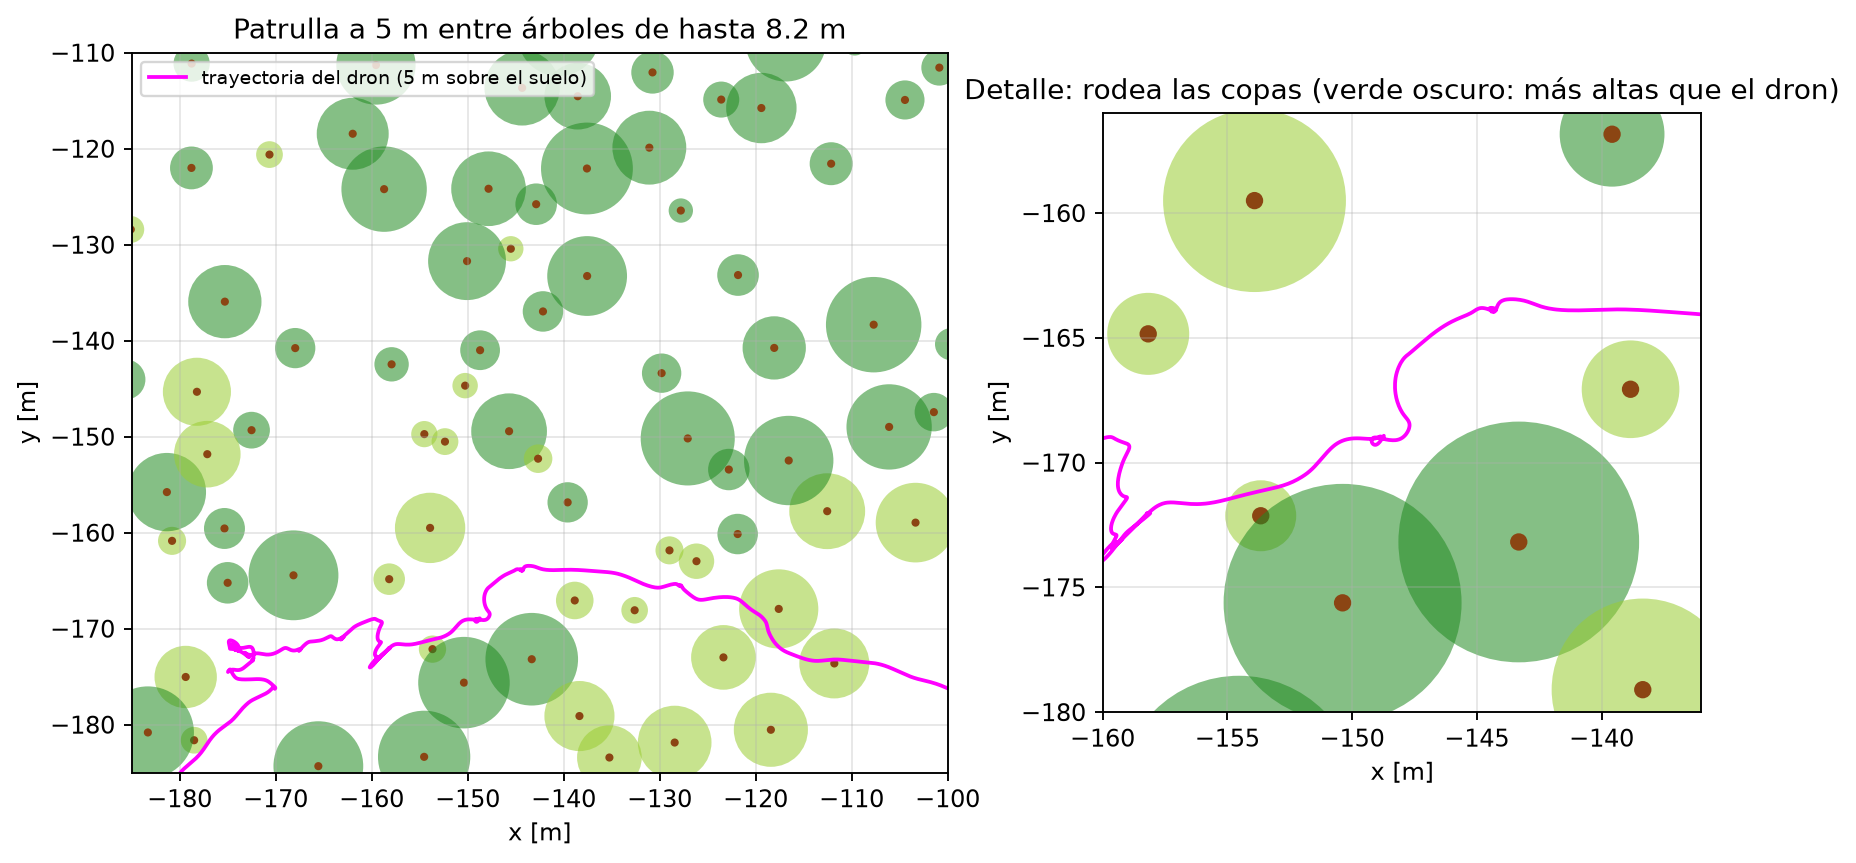
\includegraphics[width=\textwidth]{evasion_bajo.png}
\caption{Trayectoria real del dron (odometría de Gazebo) en la prueba a 5~m sobre el suelo. Los
círculos son las copas: verde oscuro, más altas que el dron.}
\end{figure}

\section{Parámetros del planificador}

\begin{longtable}{>{\raggedright\arraybackslash}p{4.3cm}>{\raggedright\arraybackslash}p{2.6cm}p{8.2cm}}
\toprule
\textbf{Parámetro} & \textbf{Valor} & \textbf{Significado} \\ \midrule \endhead
\cod{zona} & $[-210, 210]^2$ & rectángulo del bosque que se recorre [m] \\
\cod{patron} & serpentina & \cod{serpentina} o \cod{franjas} \\
\cod{separacion} & 70 & entre barridos [m] \\
\cod{anticipo_ruta} & 10 & distancia del punto que persigue sobre la ruta [m] \\
\cod{altura_busqueda} & 30 & sobre el suelo [m] \\
\cod{anticipacion} & 50 & mira el relieve esta distancia adelante [m] \\
\cod{velocidad}, \cod{velocidad_vertical} & 5, 3 & [m/s] \\
\cod{aceleracion} & 1.5 & [m/s$^2$] \\
\cod{alcance_vision} & 150 & para la cobertura [m] \\
\cod{alcance_llamas} & 100 & solo usa cortes de llamas más cercanos [m] \\
\cod{altura_orbita}, \cod{altura_minima_copas} & 18, 14 & órbita sobre el foco y sobre el anillo [m] \\
\cod{radio}, \cod{omega} & 14, 0.12 & órbita [m], [rad/s] \\
\cod{radio_verificacion}, \cod{tiempo_verificacion} & 35, 120 & [m], [s] \\
\cod{altura_seguridad} & 10 & sobre el relieve que tiene adelante [m] \\
\cod{radio_evasion}, \cod{alcance_evasion} & 3, 20 & [m] \\
\cod{evasion} & true & activa la evasión con el LiDAR \\
\cod{origen_gps} & (19.293, $-$99.311, 3000) & latitud, longitud y altitud del origen \\
\cod{registro_incendios} & \cod{~/incendios_detectados.csv} & CSV de avisos \\
\bottomrule
\end{longtable}

\chapter{¿Qué es un piloto automático? ArduPilot y MAVLink}
\label{cap:autopiloto}

\begin{enpocas}
Qué hace el software de un controlador de vuelo, qué son los modos de vuelo, por qué el dron tiene que
``armarse'', qué es el EKF, cómo se comunica con tierra (MAVLink) y para qué sirve una estación de
tierra.
\end{enpocas}

\section{El software del controlador de vuelo}

Los drones reales no corren un controlador escrito desde cero: usan un \textbf{piloto automático} de
código abierto ya probado en millones de horas de vuelo. Los dos más usados son \textbf{ArduPilot}
(su versión para multirrotores se llama ArduCopter) y \textbf{PX4}. Hacen todo lo de los capítulos
anteriores y más:
\begin{itemize}
  \item estiman dónde está el dron y cómo está orientado combinando sensores;
  \item controlan posición, velocidad y actitud (con PID en cascada);
  \item ofrecen modos de vuelo, misiones con puntos de paso y regreso a casa;
  \item vigilan la seguridad: batería, señal de radio, GPS, geocercas.
\end{itemize}
Aquí se usa ArduCopter 4.7.2 como \textbf{referencia}: comparar el STA contra un piloto
automático profesional es más convincente que compararlo solo contra un PD hecho en casa.

\section{Modos de vuelo}

ArduCopter tiene más de veinte modos. Los que aparecen en este proyecto:
\begin{description}
  \item[STABILIZE:] el piloto controla la inclinación con la palanca; el dron solo se mantiene
        nivelado.
  \item[LOITER:] el dron se queda en su lugar usando el GPS.
  \item[GUIDED:] el dron obedece órdenes de una computadora (``ve a este punto'', ``mantén esta
        velocidad''). Es el que usa nuestra misión.
  \item[RTL] (\emph{return to launch}): regresa a donde despegó y aterriza.
  \item[LAND:] aterriza donde está.
\end{description}

\section{Armar el dron}

Por seguridad, los motores no giran hasta que el dron se \textbf{arma}. Antes de permitirlo, ArduPilot
revisa (\emph{pre-arm checks}) que los sensores estén calibrados, que el GPS tenga buena señal, que la
batería esté bien y que el estimador esté listo. Por eso la misión con ArduPilot espera unos 30
segundos antes de despegar.

\section{El EKF: adivinar bien dónde estoy}

Ningún sensor es perfecto: el GPS da la posición con metros de error y pocas veces por segundo; la IMU
es rápida pero sus errores se acumulan; el barómetro deriva con el clima. El \textbf{filtro de Kalman
extendido} (EKF) los combina: predice con la IMU y corrige con el GPS, el barómetro y la brújula,
pesando cada uno según su confianza. ArduPilot usa la versión EKF3.

\begin{ejemplo}
Caminar con los ojos cerrados contando pasos (la IMU) te lleva más o menos a donde quieres, pero el
error crece. Si de vez en cuando abres los ojos un instante (el GPS), corriges. El EKF hace eso
cientos de veces por segundo.
\end{ejemplo}

\section{MAVLink: el idioma de los drones}

\textbf{MAVLink} es el protocolo con el que el piloto automático habla con el exterior: mensajes
pequeños y bien definidos como \cod{HEARTBEAT} (``sigo vivo''), \cod{GLOBAL_POSITION_INT} (posición
GPS), \cod{COMMAND_LONG} (``despega'') o \cod{SET_POSITION_TARGET_LOCAL_NED} (``ve a este punto'').

\begin{figure}[H]
\centering
\begin{tikzpicture}[blq/.style={draw,rounded corners,fill=#1,minimum width=3cm,minimum height=1.1cm,align=center,font=\small},
  fl/.style={{Stealth[length=2.2mm]}-{Stealth[length=2.2mm]},thick}]
  \node[blq=orange!15] (gz) at (0,0) {Gazebo\\(física, sensores)};
  \node[blq=red!10] (ap) at (4.5,0) {ArduCopter SITL\\(EKF, control, modos)};
  \node[blq=black!5] (mp) at (9,0) {MAVProxy\\(estación de tierra)};
  \node[blq=green!12] (mi) at (9,-2.4) {\cod{mision_ardupilot}\\(nuestra misión)};
  \node[blq=green!12] (bus) at (4.5,-2.4) {\cod{busqueda_incendio}};
  \node[blq=blue!8] (qgc) at (13,0) {QGroundControl\\(opcional)};
  \draw[fl] (gz) -- node[above,font=\scriptsize]{JSON / UDP} (ap);
  \draw[fl] (ap) -- node[above,font=\scriptsize]{MAVLink} (mp);
  \draw[fl] (mp) -- node[right,font=\scriptsize]{MAVLink (UDP 14551)} (mi);
  \draw[fl] (mp) -- node[above,font=\scriptsize]{UDP 14550} (qgc);
  \draw[-{Stealth[length=2.2mm]},thick] (bus) -- node[above,font=\scriptsize]{consigna (ROS 2)} (mi);
\end{tikzpicture}
\caption{Cómo se conectan las piezas al volar con ArduPilot SITL.}
\end{figure}

\section{Estación de tierra}

Una \textbf{estación de tierra} (GCS) es el programa con el que una persona ve y manda al dron:
mapa, telemetría, botones para cambiar de modo. Usamos \textbf{MAVProxy}, que trae consola, mapa y
un prompt donde se escriben comandos (\cod{mode GUIDED}, \cod{arm throttle}, \cod{mode RTL}...).
También se puede conectar QGroundControl por el puerto UDP 14550.

\begin{recuerda}
Con \cod{controlador:=ardupilot}, nuestros controladores de ROS no se usan: el que pilota es ArduCopter.
Nuestro planificador sigue decidiendo a dónde ir y se lo pide a ArduCopter en modo GUIDED, exactamente
como se haría con el dron real conectado a una computadora a bordo.
\end{recuerda}

\chapter{Volar la búsqueda con ArduPilot}

\begin{enpocas}
Cómo se conectó ArduCopter a nuestra simulación: el modelo del dron para ArduPilot, sus parámetros, el nodo de misión, las ventanas, los comandos y la trayectoria en el mapa.
\end{enpocas}

\begin{lstlisting}[style=bash]
ros2 launch cuadrirotor_sim simulacion.launch.py vehiculo:=tarot650 mundo:=bosque_grande \
    controlador:=ardupilot mision:=busqueda
\end{lstlisting}

Con \cod{controlador:=ardupilot} el dron lo pilota ArduCopter 4.7.2 en lugar de los
controladores de ROS~2. Así se puede comparar el STA con un piloto automático real y
probar la misión con la misma interfaz (MAVLink) que tendría el dron físico.

\section{El vehículo para ArduPilot}
\label{sec:plugin-ap}

\cod{generar_modelo.py} genera también \cod{models/tarot650_ardupilot}: el mismo Tarot con
\begin{itemize}
  \item el plugin \cod{ArduPilotPlugin} (de \cod{ardupilot_gazebo}), que intercambia con el SITL el
        estado del dron y las salidas de los motores por UDP (puerto 9002, formato JSON, en
        \emph{lock-step}) y lee una IMU girada al marco NED;
  \item el sistema \cod{ComandosMotores} (\cod{cuadrirotor_gz_plugins}), que junta las cuatro salidas
        (un \cod{gz.msgs.Double} por motor, PWM de 1000--2000~µs escalado a 0--680~rad/s) en un solo
        \cod{gz.msgs.Actuators}, que es lo que espera \cod{MulticopterMotorModel}.
\end{itemize}
Así la física de los motores, el viento y el incendio son los mismos que con el PD y el STA.

\begin{lstlisting}[style=xml]
<plugin filename="ArduPilotPlugin" name="ArduPilotPlugin">
  <fdm_addr>127.0.0.1</fdm_addr>
  <fdm_port_in>9002</fdm_port_in>
  <lock_step>1</lock_step>
  <modelXYZToAirplaneXForwardZDown degrees="true">0 0 0 180 0 0</modelXYZToAirplaneXForwardZDown>
  <gazeboXYZToNED degrees="true">0 0 0 180 0 90</gazeboXYZToNED>
  <imuName>base_link::imu_sensor</imuName>
  <control channel="0">
    <jointName>rotor_0_joint</jointName>
    <type>COMMAND</type>
    <cmd_topic>/cuadrirotor/ap/motor_0</cmd_topic>
    <multiplier>680.0</multiplier>
    <servo_min>1000</servo_min>
    <servo_max>2000</servo_max>
  </control>
  <!-- ... canales 1 a 3 ... -->
</plugin>
<plugin filename="ComandosMotores" name="cuadrirotor::ComandosMotores">
  <entrada>/cuadrirotor/ap/motor_0</entrada>  <!-- ... motor_1 a motor_3 -->
  <salida>/cuadrirotor/command/motor_speed</salida>
</plugin>
\end{lstlisting}

\section{Parámetros de ArduCopter}

\cod{config/ardupilot/tarot650.parm} se carga sobre los del Iris de \cod{ardupilot_gazebo}:

\begin{lstlisting}
FRAME_CLASS     1        # quad
FRAME_TYPE      1        # X
MOT_PWM_MIN     1000
MOT_PWM_MAX     2000
MOT_THST_EXPO   1.0      # salida lineal en w, empuje en w^2: curva cuadrática pura
MOT_SPIN_ARM    0.08
MOT_SPIN_MIN    0.12
MOT_THST_HOVER  0.28     # (357/680)^2
MOT_HOVER_LEARN 2
ATC_RAT_RLL_P   0.08     # lazos de tasa más suaves que el Iris:
ATC_RAT_RLL_I   0.08     # empuje/peso ~3.6 y motores más lentos (30-50 ms)
ATC_RAT_RLL_D   0.002
ATC_RAT_PIT_P   0.08
ATC_RAT_PIT_I   0.08
ATC_RAT_PIT_D   0.002
ATC_RAT_YAW_P   0.2
ATC_RAT_YAW_I   0.02
\end{lstlisting}

\section{El nodo \texorpdfstring{\texttt{mision\_ardupilot}}{mision\_ardupilot}}

Corre con el Python de \cod{~/venv-ardupilot} (pymavlink) y se conecta a MAVProxy por
\cod{udp:127.0.0.1:14551}. Espera a que el EKF esté listo, pone el modo GUIDED, arma y despega con
\cod{MAV_CMD_NAV_TAKEOFF}. Después manda a 20~Hz \cod{SET_POSITION_TARGET_LOCAL_NED} con posición,
velocidad y guiñada:
\begin{itemize}
  \item con \cod{mision:=orbita} o \cod{hover}, la misma referencia que los controladores de ROS~2
        (\cod{dinamica.Referencia}); guarda el CSV con \cod{csv:=} en el formato de \cod{metricas.py};
  \item con \cod{mision:=busqueda}, despega a 5~m y después reenvía las consignas de
        \cod{busqueda_incendio}.
\end{itemize}
El paso de ENU a NED es $N = y$, $E = x$, $D = -z$ y $\psi_{NED} = \pi/2 - \psi$.

\begin{leccion}
Con el backend JSON, el marco local de ArduPilot (\cod{LOCAL_POSITION_NED}) \textbf{es} el mundo de
Gazebo, y el GPS de ArduPilot es el \emph{home} más la posición en Gazebo. La primera versión
restaba además el punto de salida $(-232,-232)$: todas las consignas llegaban corridas $\approx$330~m
al noreste. El dron patrullaba fuera de su ruta (de ahí unas detecciones de humo en rumbos
extraños) y en una corrida se estrelló contra un cerro (``\emph{Crash: Disarming}'').
Se encontró comparando el tlog de MAVProxy con la odometría de Gazebo. Ahora:
\begin{itemize}
  \item antes de armar se mide el desfase entre \cod{LOCAL_POSITION_NED} y la odometría (sale
        $\approx$(0.02, 0.01, 0.01)~m) y se descuenta, en lugar de suponerlo;
  \item el \emph{home} del SITL (\cod{-l}) es el origen del mundo (\cod{geo.ORIGEN}), así que el GPS
        de ArduPilot coincide con el del aviso del incendio.
\end{itemize}
\end{leccion}

\section{Las ventanas del SITL}
\label{sec:ventanas}

Con GUI se abren cinco ventanas, que \cod{ventanas_sitl.py} acomoda en columnas cuando aparecen
(con \cod{python-xlib}, por EWMH): la terminal \textbf{MAVProxy} arriba a la izquierda y al frente,
la consola y la terminal de ArduCopter debajo, Gazebo al centro y el mapa a la derecha.

\begin{figure}[H]
\centering
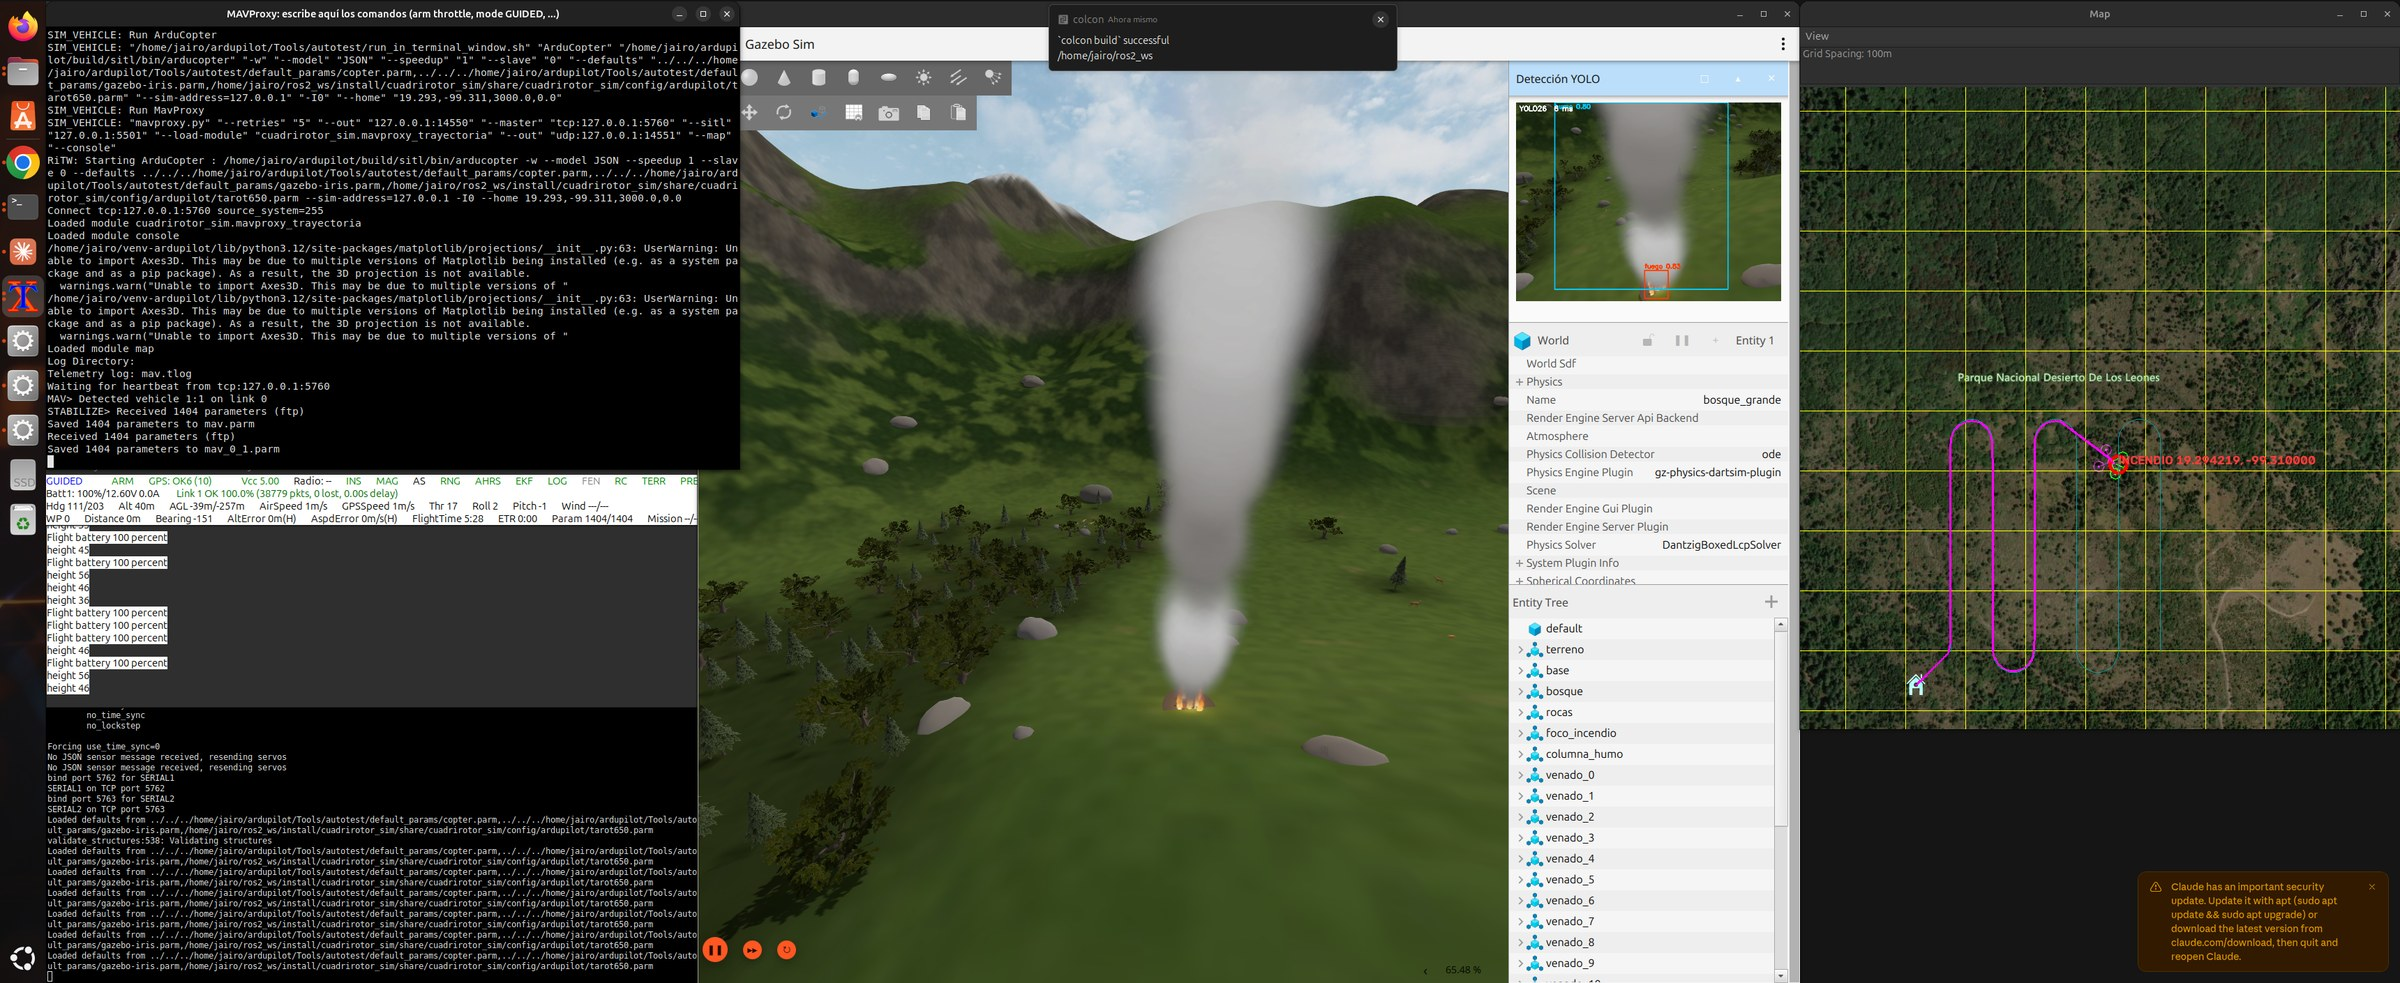
\includegraphics[width=\textwidth]{sitl_pantalla.jpg}
\caption{Pantalla durante la búsqueda con ArduPilot, al confirmarse el incendio.}
\end{figure}

\begin{description}
  \item[Terminal MAVProxy] sim\_vehicle.py corre dentro de ella: ahí queda el prompt de MAVProxy
        para escribir comandos.
  \item[Consola de MAVProxy] modo, armado, GPS, batería, altura y mensajes de ArduPilot.
  \item[Terminal ArduCopter] el proceso del SITL (antes se abría minimizada; ahora,
        \cod{SITL_RITW_TERMINAL} la abre a la vista).
  \item[Mapa] imagen satelital con el dron, el \emph{home} y lo que dibuja
        \cod{mavproxy_trayectoria}.
\end{description}

\begin{figure}[H]
\centering
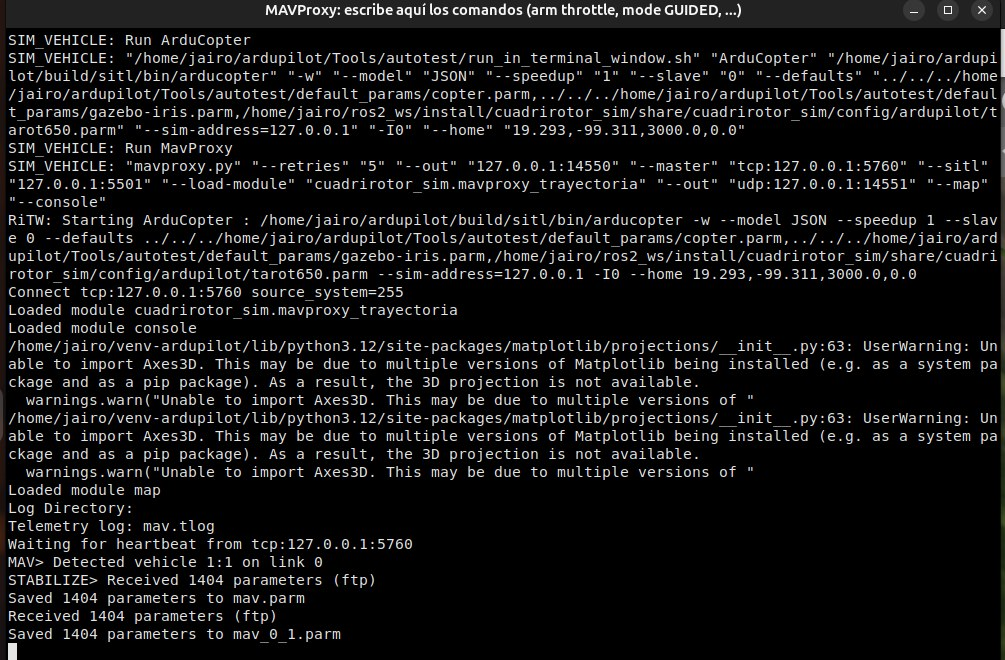
\includegraphics[width=0.56\textwidth]{sitl_mavproxy.jpg}\hfill
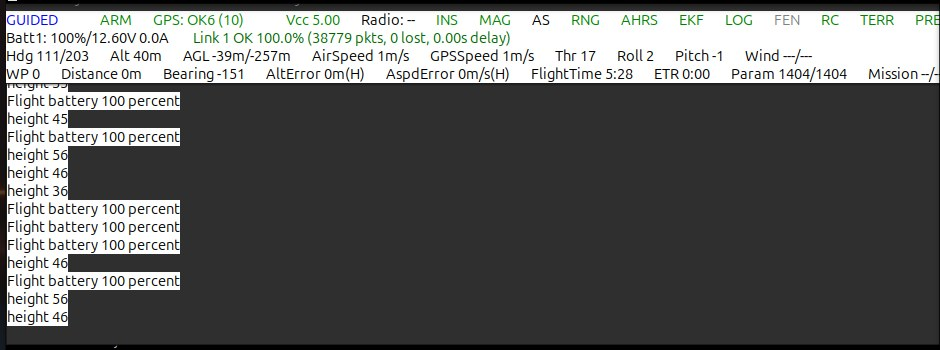
\includegraphics[width=0.42\textwidth]{sitl_consola.jpg}
\caption{Terminal de MAVProxy con su prompt (izquierda) y consola (derecha).}
\end{figure}

\subsection{Comandos útiles en el prompt de MAVProxy}

\begin{longtable}{>{\raggedright\arraybackslash}p{5cm}p{10cm}}
\toprule
\textbf{Comando} & \textbf{Efecto} \\ \midrule \endhead
\cod{mode GUIDED} & modo guiado (el que usa la misión) \\
\cod{arm throttle} & arma los motores \\
\cod{takeoff 10} & despega a 10~m (en GUIDED y armado) \\
\cod{mode LOITER} / \cod{mode BRAKE} & se queda en el lugar \\
\cod{mode RTL} & regresa a la base y aterriza \\
\cod{mode LAND} & aterriza donde está \\
\cod{disarm} & desarma (en tierra) \\
\cod{param show MOT_*} / \cod{param set NOMBRE valor} & ver y cambiar parámetros \\
\cod{trayectoria borrar} / \cod{ocultar} / \cod{mostrar} & controla el dibujo de la trayectoria en el mapa \\
\bottomrule
\end{longtable}

\begin{aviso}
Si se toma el control desde MAVProxy (por ejemplo \cod{mode RTL}), \cod{mision_ardupilot} sigue
enviando consignas, que solo surten efecto en GUIDED: al volver a \cod{mode GUIDED} el dron retoma
la búsqueda.
\end{aviso}

\section{La trayectoria en el mapa}

El módulo de MAVProxy \cod{cuadrirotor_sim.mavproxy_trayectoria} (se carga con
\cod{--load-module} cuando hay GUI) dibuja:
\begin{itemize}
  \item en magenta, \textbf{toda} la trayectoria recorrida (un punto cada 2~m de la posición GPS),
        en lugar de la estela de 12~s que trae MAVProxy;
  \item en cian, la ruta planeada (la serpentina);
  \item un círculo rojo con las coordenadas cuando se confirma el incendio.
\end{itemize}
La ruta y el foco los escribe \cod{busqueda_incendio} en
\cod{/tmp/cuadrirotor_sim_<uid>/mapa_busqueda.json}; el módulo lo vuelve a leer cuando cambia.

\begin{figure}[H]
\centering
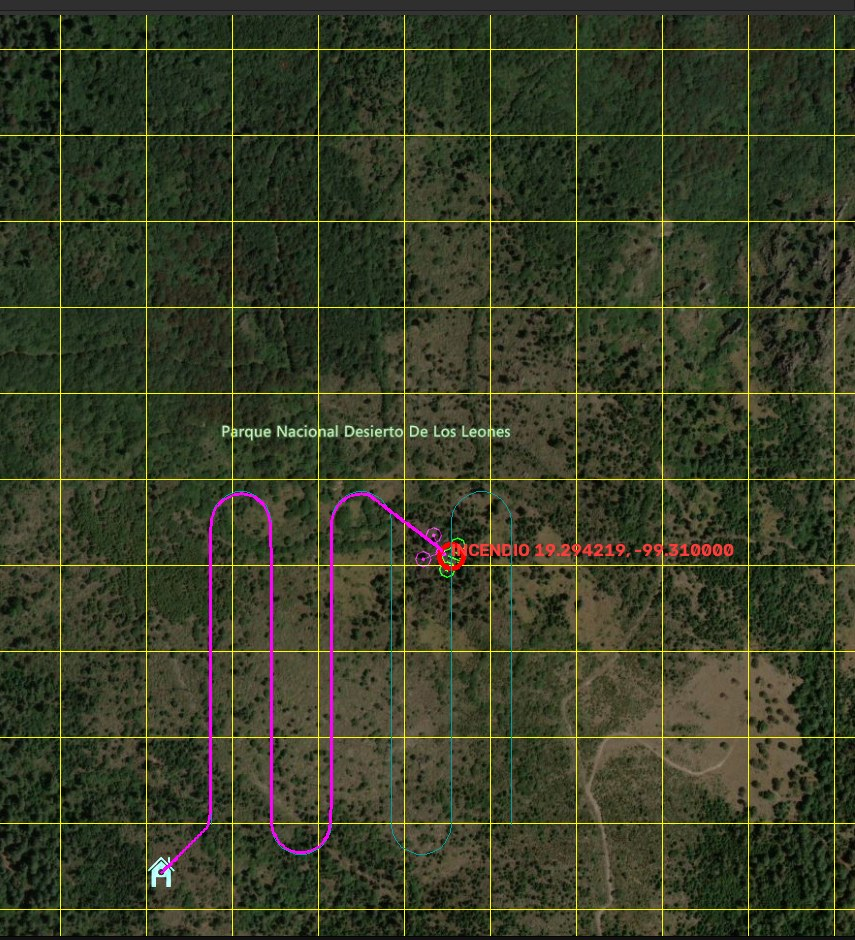
\includegraphics[width=0.6\textwidth]{mapa_trayectoria.jpg}
\caption{Mapa de MAVProxy al final de la búsqueda: trayectoria recorrida desde la base (H), ruta
planeada y foco confirmado.}
\end{figure}

\section{Cierre limpio}

Al cerrar el \emph{launch} con Ctrl-C, un manejador \cod{OnShutdown} termina lo que no se cierra
solo: el \cod{gz sim} que queda detrás del envoltorio de ruby (que no reenvía la señal) y, con
ArduPilot, MAVProxy y ArduCopter, que sim\_vehicle no cierra cuando se cierra su terminal.


\part{Manos a la obra}
\chapter{Tu primer vuelo, paso a paso}
\label{cap:primer-vuelo}

\begin{enpocas}
Un recorrido guiado: despegar y mantener el dron en el aire, mirar qué pasa por dentro, hacer una
órbita con viento y medirla, lanzar la búsqueda autónoma del incendio y, al final, volar con ArduPilot
y darle órdenes desde MAVProxy. Supone que la instalación (capítulo~\ref{cap:instalacion}) ya está hecha.
\end{enpocas}

\section{Paso 0: preparar la terminal}

Abre una terminal y escribe:
\begin{lstlisting}[style=bash]
source /opt/ros/jazzy/setup.bash
source ~/ros2_ws/install/setup.bash
\end{lstlisting}
Hazlo en \emph{cada} terminal nueva (o agrégalo a \cod{~/.bashrc}).

\section{Paso 1: despegar}

\begin{lstlisting}[style=bash]
ros2 launch cuadrirotor_sim simulacion.launch.py vehiculo:=tarot650 mundo:=bosque_grande controlador:=sta mision:=hover
\end{lstlisting}

Se abre Gazebo. El Tarot aparece sobre la base, despega suavemente y se queda a 3~m. A los 12 segundos
la cámara de la ventana empieza a seguirlo. En la terminal verás mensajes de los nodos.

\begin{figure}[H]
\centering
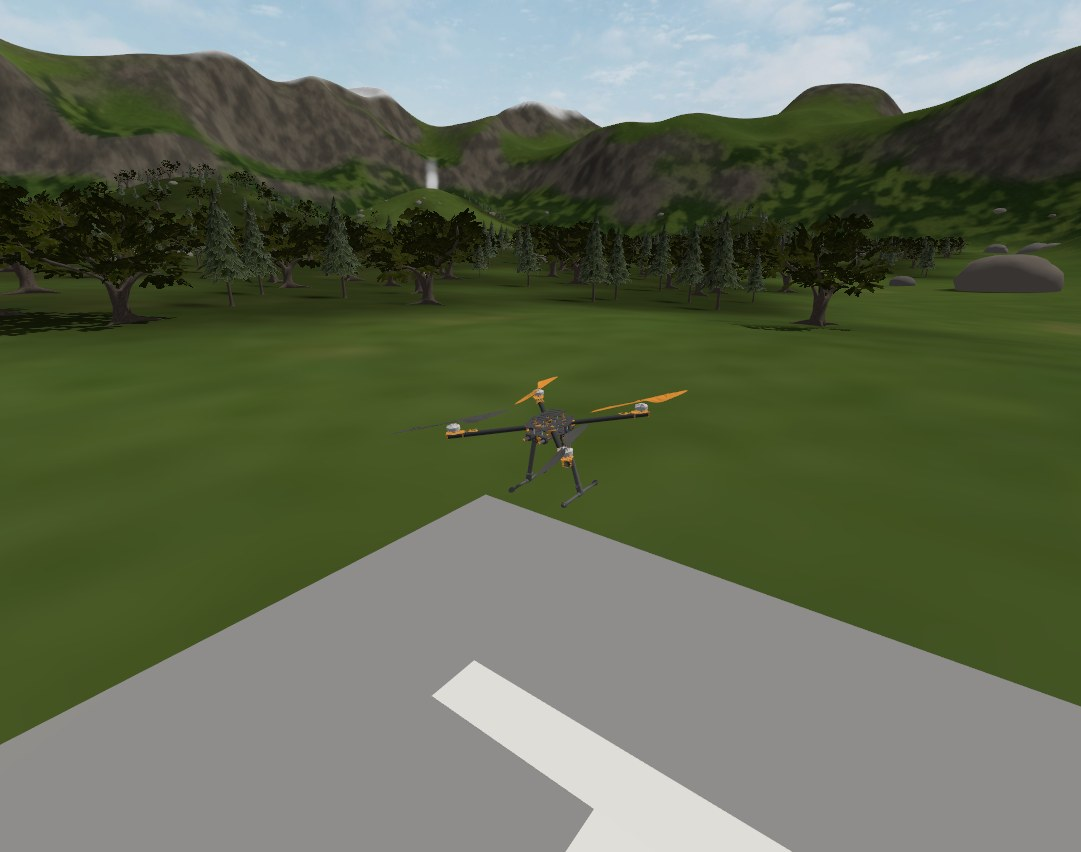
\includegraphics[width=0.75\textwidth]{gz_tarot_cerca.jpg}
\caption{Lo que debes ver: el Tarot en vuelo estacionario sobre la base.}
\end{figure}

\begin{consejo}
En Gazebo: rueda del ratón = acercar; botón izquierdo arrastrando = girar la vista; botón derecho
(o Shift + izquierdo) = desplazar. El botón ``play/pausa'' de abajo a la izquierda congela la física.
\end{consejo}

\section{Paso 2: mirar por dentro}

Abre una segunda terminal (con el Paso~0) y explora:
\begin{lstlisting}[style=bash]
ros2 node list                                                 # ¿quién está corriendo?
ros2 topic list                                                # ¿qué datos circulan?
ros2 topic echo /cuadrirotor/odometria --field pose.pose.position   # la posición del dron
ros2 topic echo /cuadrirotor/error                             # el error de seguimiento
ros2 run rqt_image_view rqt_image_view /cuadrirotor/camara     # lo que ve la cámara
\end{lstlisting}

\begin{figure}[H]
\centering
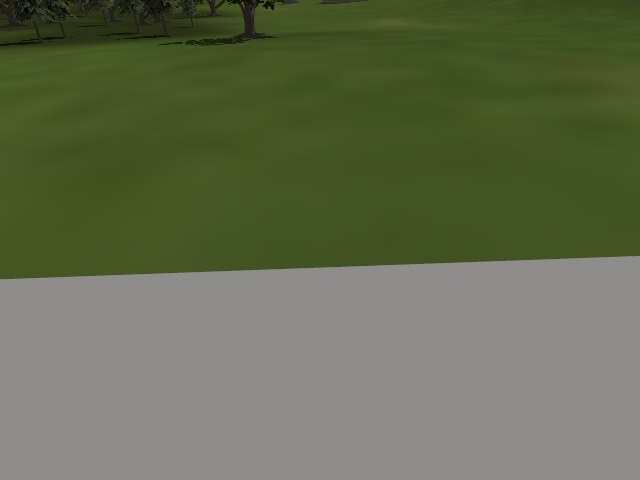
\includegraphics[width=0.6\textwidth]{gz_camara_dron.jpg}
\caption{La imagen de la cámara del dron sobre la base: el borde de la losa y el pasto.}
\end{figure}

Para cerrar la simulación, regresa a la primera terminal y presiona \textbf{Ctrl+C}.

\section{Paso 3: una órbita con viento, y medirla}

\begin{lstlisting}[style=bash]
ros2 launch cuadrirotor_sim simulacion.launch.py vehiculo:=tarot650 mundo:=bosque \
    controlador:=sta esquema:=implicito mision:=orbita viento:=true csv:=$HOME/mi_orbita.csv
\end{lstlisting}

El dron despega, va junto al foco del incendio y le da vueltas a 4~m de radio mirándolo; a los 15~s
empieza a soplar viento. Déjalo un par de minutos, ciérralo con Ctrl+C y mide:
\begin{lstlisting}[style=bash]
python3 ~/ros2_ws/src/cuadrirotor_sim/scripts/metricas.py ~/mi_orbita.csv
\end{lstlisting}
Verás el error RMS sin viento y con viento (unos 3 y 5~cm con el STA). Repite con
\cod{controlador:=pd} y compara: es el experimento central del proyecto.

\begin{ejercicio}
Abre \cod{~/mi_orbita.csv} en una hoja de cálculo o con Python y grafica \cod{x} contra \cod{y}: verás
el círculo de la órbita. Las columnas \cod{sx}, \cod{sy}, \cod{sz} son la variable deslizante y
\cod{k1x}, \cod{k1y}, \cod{k1z}, la ganancia adaptativa.
\end{ejercicio}

\section{Paso 4: la búsqueda autónoma del incendio}

\begin{lstlisting}[style=bash]
ros2 launch cuadrirotor_sim simulacion.launch.py vehiculo:=tarot650 mundo:=bosque_grande \
    controlador:=sta mision:=busqueda
\end{lstlisting}

Ahora el dron va solo:
\begin{enumerate}
  \item despega a 30~m sobre el suelo;
  \item recorre el bosque en serpentina (en la terminal: \emph{[patrulla] Recorriendo el bosque});
  \item cuando YOLO ve humo, se dirige hacia él (\emph{[hacia\_humo]});
  \item estima dónde está el foco y se acerca (\emph{[aproximacion]});
  \item al confirmarlo con las llamas, baja y empieza a orbitar, y escribe el aviso:
\end{enumerate}
\begin{lstlisting}
INCENDIO CONFIRMADO 2026-10-23 04:26:47
  GPS: 19.294219, -99.310000  (19°17'39.2"N 99°18'36.0"W)
  Mapa: https://www.google.com/maps?q=19.294219,-99.310000
\end{lstlisting}
Tarda entre uno y tres minutos según dónde esté el fuego. En la ventana de Gazebo, el panel
``Detección YOLO'' muestra lo que ve la red neuronal.

\begin{figure}[H]
\centering
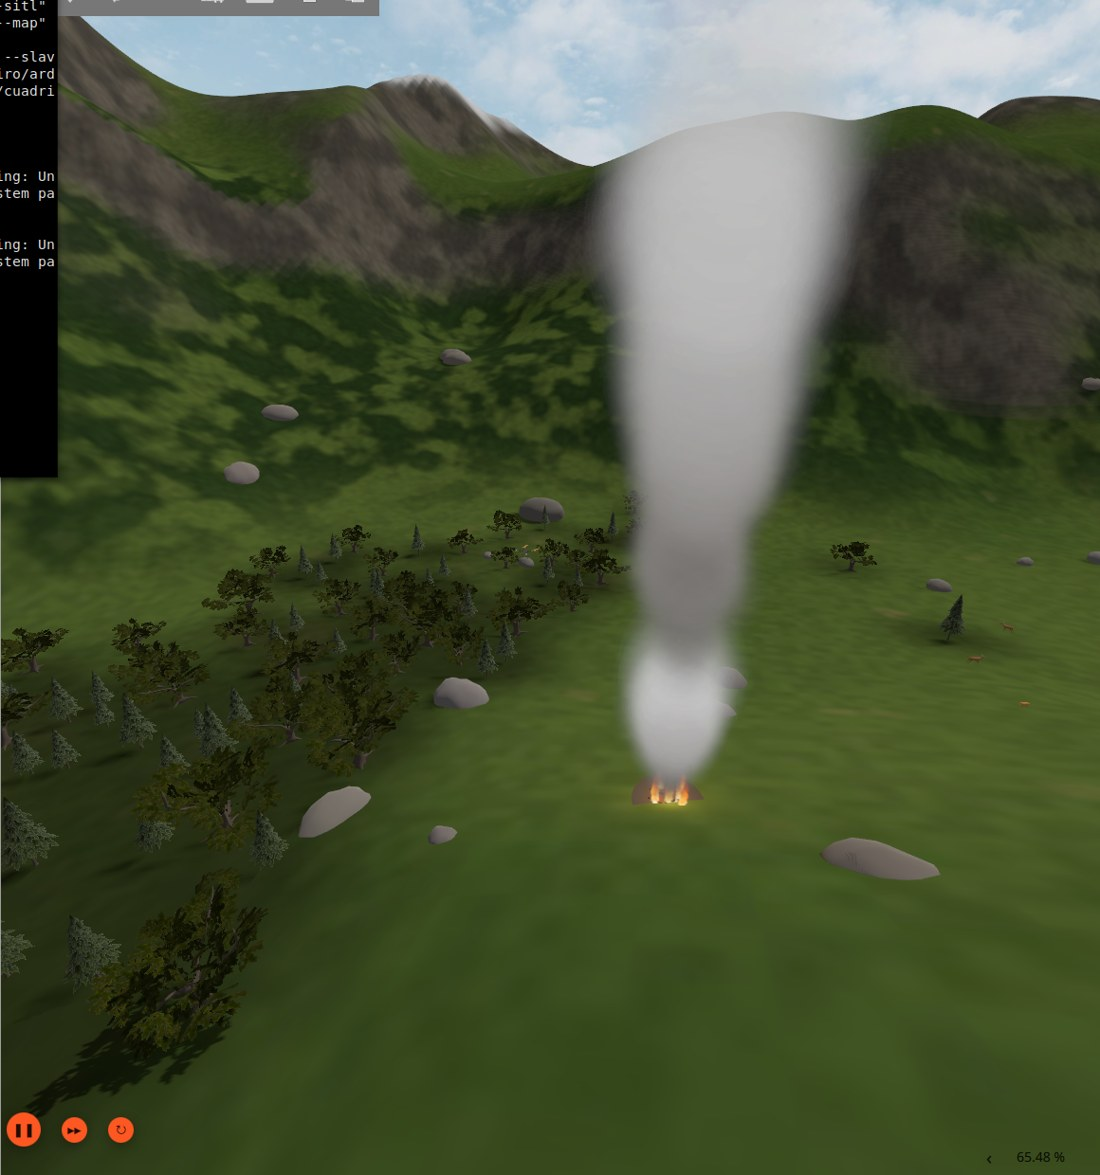
\includegraphics[width=0.6\textwidth]{gazebo_humo.jpg}
\caption{El dron llegando al incendio.}
\end{figure}

\begin{ejercicio}
Pon el incendio en otro lugar y observa cuánto tarda en encontrarlo:
\begin{lstlisting}[style=bash]
ros2 launch cuadrirotor_sim simulacion.launch.py vehiculo:=tarot650 mundo:=bosque_grande \
    controlador:=sta mision:=busqueda foco_x:=-150 foco_y:=60
\end{lstlisting}
Desde otra terminal: \cod{ros2 topic echo /cuadrirotor/busqueda/cobertura} muestra qué porcentaje del
bosque ya vio.
\end{ejercicio}

\section{Paso 5: volar con ArduPilot y darle órdenes}

\begin{lstlisting}[style=bash]
ros2 launch cuadrirotor_sim simulacion.launch.py vehiculo:=tarot650 mundo:=bosque_grande \
    controlador:=ardupilot mision:=busqueda
\end{lstlisting}

Se abren cinco ventanas acomodadas solas: arriba a la izquierda la terminal \textbf{MAVProxy}, debajo
la consola y la terminal de ArduCopter, Gazebo al centro y el mapa a la derecha. Tras $\approx$30~s de
revisiones, ArduPilot arma, despega y sigue la misma búsqueda. En el mapa verás la ruta planeada en
cian y lo recorrido en magenta.

\begin{figure}[H]
\centering
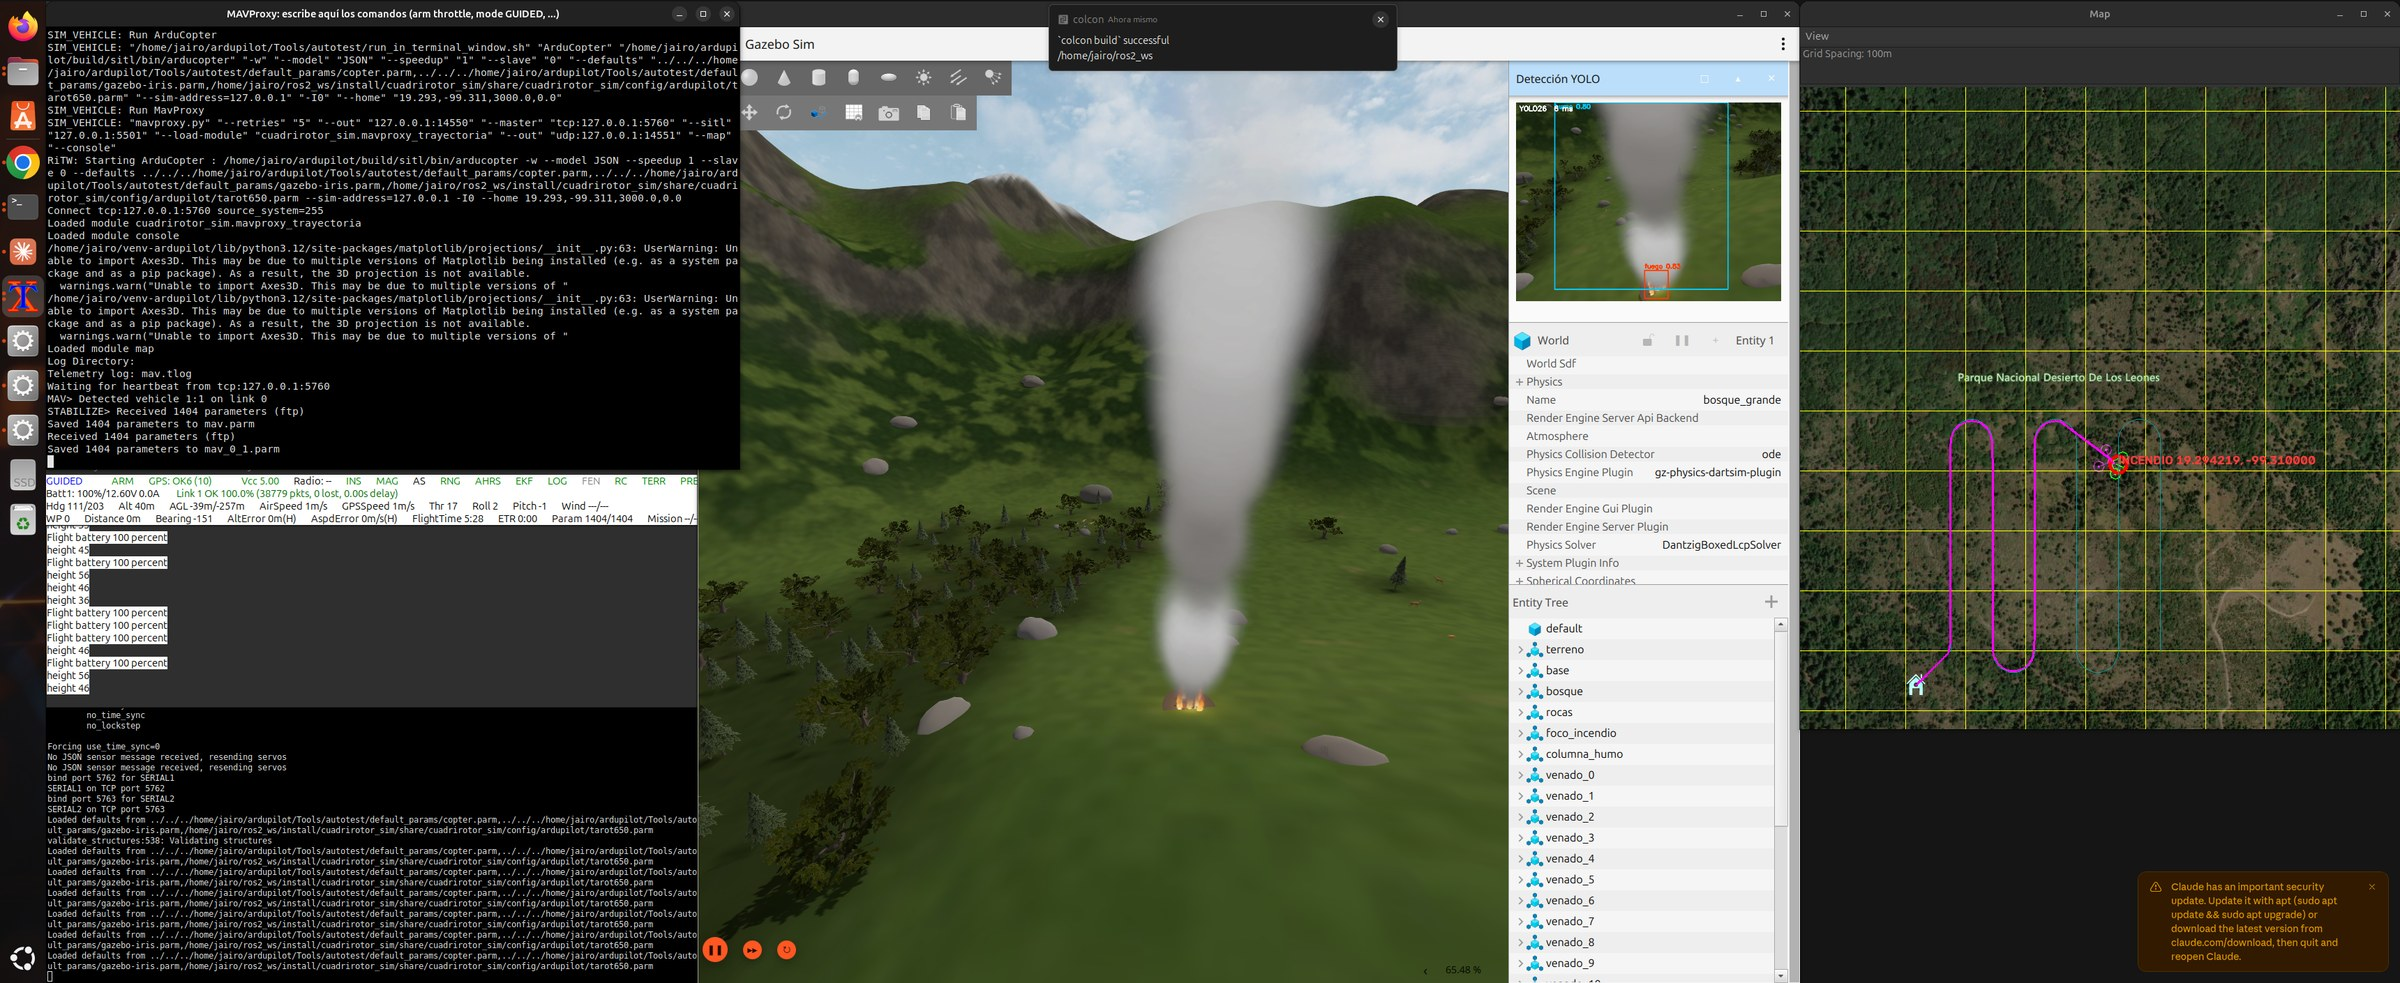
\includegraphics[width=\textwidth]{sitl_pantalla.jpg}
\caption{La pantalla con ArduPilot al confirmarse el incendio.}
\end{figure}

Escribe en la terminal MAVProxy (donde dice \cod{MAV>} o \cod{GUIDED>}):
\begin{lstlisting}
mode LOITER          # el dron se detiene donde está
mode GUIDED          # retoma la búsqueda
mode RTL             # regresa a la base y aterriza
trayectoria borrar   # limpia la línea magenta del mapa
\end{lstlisting}

\begin{aviso}
Si tomas el control con un modo distinto de GUIDED, la misión no puede mover al dron hasta que
regreses a \cod{mode GUIDED}. Y si aterriza con RTL y se desarma, hay que reiniciar la simulación.
\end{aviso}

\section{Qué hacer si algo falla}

\begin{longtable}{>{\raggedright\arraybackslash}p{5.5cm}p{9.5cm}}
\toprule
\textbf{Síntoma} & \textbf{Qué revisar} \\ \midrule \endhead
\emph{Package 'cuadrirotor\_sim' not found} & Falta \cod{source ~/ros2_ws/install/setup.bash} en esa terminal. \\
Gazebo abre pero el dron no aparece & Mira la terminal: un error en rojo del \emph{launch} dice qué falló. \\
La simulación va muy lenta & Cierra otros programas; prueba \cod{gui:=false}. Revisa el factor de tiempo real abajo a la derecha de Gazebo. \\
YOLO no detecta nada & ¿Existe \cod{~/.venvs/yolo}? ¿Tiene GPU? Mira los mensajes de \cod{detector_yolo}. \\
Quedan procesos de una simulación anterior & Ciérrala con Ctrl+C y espera unos segundos; si algo queda, búscalo con \cod{ps aux | grep gz} y termínalo por su número (PID). \\
ArduPilot no arma & Espera: el EKF tarda $\approx$30~s. La consola de MAVProxy dice qué revisión falla. \\
\bottomrule
\end{longtable}

\chapter{Referencia de uso}

\begin{enpocas}
Todas las órdenes, argumentos y tópicos en un solo lugar, para consultar.
\end{enpocas}

\section{Antes de lanzar}

\begin{lstlisting}[style=bash]
cd ~/ros2_ws
colcon build --symlink-install      # solo si se agregaron ejecutables o se cambió C++
source install/setup.bash
\end{lstlisting}

\section{Órdenes de lanzamiento}

\begin{lstlisting}[style=bash]
# Cuadrirrotor genérico: despegue y hover a 3 m
ros2 launch cuadrirotor_sim simulacion.launch.py

# Órbita alrededor del foco con viento, guardando un CSV
ros2 launch cuadrirotor_sim simulacion.launch.py mision:=orbita viento:=true csv:=$HOME/corrida.csv

# STA implícito, Tarot, bosque
ros2 launch cuadrirotor_sim simulacion.launch.py vehiculo:=tarot650 mundo:=bosque \
    controlador:=sta esquema:=implicito mision:=orbita viento:=true

# Sin interfaz y con otro periodo de muestreo
ros2 launch cuadrirotor_sim simulacion.launch.py gui:=false Ts:=0.01

# Búsqueda autónoma del incendio en el valle (STA)
ros2 launch cuadrirotor_sim simulacion.launch.py vehiculo:=tarot650 mundo:=bosque_grande \
    controlador:=sta mision:=busqueda
#   ... con el foco en otro lugar
ros2 launch cuadrirotor_sim simulacion.launch.py vehiculo:=tarot650 mundo:=bosque_grande \
    controlador:=sta mision:=busqueda foco_x:=-150 foco_y:=60

# La misma búsqueda pilotada por ArduPilot SITL
ros2 launch cuadrirotor_sim simulacion.launch.py vehiculo:=tarot650 mundo:=bosque_grande \
    controlador:=ardupilot mision:=busqueda
\end{lstlisting}

\section{Argumentos del \emph{launch}}

\begin{longtable}{>{\raggedright\arraybackslash}p{2.6cm}>{\raggedright\arraybackslash}p{2.6cm}p{9.8cm}}
\toprule
\textbf{Argumento} & \textbf{Por omisión} & \textbf{Valores} \\ \midrule \endhead
\cod{vehiculo} & cuadrirotor & \cod{cuadrirotor}, \cod{tarot650} \\
\cod{mundo} & incendio & \cod{incendio}, \cod{bosque}, \cod{bosque_grande} \\
\cod{controlador} & pd & \cod{pd}, \cod{sta}, \cod{ardupilot}, \cod{ninguno} (para lanzarlo aparte con \cod{ros2 run}) \\
\cod{esquema} & implicito & STA: \cod{explicito}, \cod{semi_implicito}, \cod{implicito} \\
\cod{mision} & hover & \cod{hover}, \cod{orbita}, \cod{busqueda} \\
\cod{gui} & true & mostrar la interfaz de Gazebo (y las ventanas del SITL) \\
\cod{Ts} & 0.005 & periodo de muestreo del controlador [s] \\
\cod{viento} & false & aplicar la perturbación de viento \\
\cod{csv} & & ruta del CSV de registro \\
\cod{foco_x}, \cod{foco_y} & & \cod{bosque_grande}: posición del incendio [m] \\
\cod{x0}, \cod{y0} & & posición inicial del dron [m] \\
\cod{modelo_yolo} & & pesos de YOLO (.pt) en lugar de \cod{yolo/incendio_yolo26n.pt} \\
\bottomrule
\end{longtable}

\section{Tópicos}

\begin{longtable}{>{\raggedright\arraybackslash}p{5.4cm}>{\raggedright\arraybackslash}p{6.6cm}p{3cm}}
\toprule
\textbf{Tópico} & \textbf{Tipo y contenido} & \textbf{Publica} \\ \midrule \endhead
\cod{/cuadrirotor/odometria} & \cod{nav_msgs/Odometry} (velocidades en el cuerpo) & Gazebo \\
\cod{/cuadrirotor/imu} & \cod{sensor_msgs/Imu} & Gazebo \\
\cod{/cuadrirotor/camara} & \cod{sensor_msgs/Image} 640$\times$480, 15~Hz & Gazebo \\
\cod{/cuadrirotor/lidar/points} & \cod{sensor_msgs/PointCloud2}, 10~Hz & Gazebo \\
\cod{/cuadrirotor/motores} & \cod{actuator_msgs/Actuators} [rad/s] & controlador \\
\cod{/cuadrirotor/viento} & \cod{geometry_msgs/Vector3} [N] & \cod{viento} \\
\cod{/cuadrirotor/referencia}, \cod{/cuadrirotor/error} & \cod{PoseStamped}, \cod{Vector3Stamped} & controlador \\
\cod{/cuadrirotor/consigna} & \cod{MultiDOFJointTrajectoryPoint} & planificador \\
\cod{/cuadrirotor/detecciones} & \cod{vision_msgs/Detection2DArray} & detector \\
\cod{/cuadrirotor/camara_yolo} & imagen con las cajas & detector \\
\cod{/cuadrirotor/foco_estimado} & \cod{geometry_msgs/PointStamped} & planificador \\
\cod{/cuadrirotor/busqueda/estado} & \cod{std_msgs/String} & planificador \\
\cod{/cuadrirotor/busqueda/cobertura} & \cod{std_msgs/Float32} (\% visto) & planificador \\
\cod{/cuadrirotor/busqueda/mapa_cobertura} & \cod{nav_msgs/OccupancyGrid} & planificador \\
\cod{/cuadrirotor/busqueda/ruta} & \cod{nav_msgs/Path} & planificador \\
\cod{/cuadrirotor/evasion/obstaculos} & \cod{sensor_msgs/PointCloud2} (marco \cod{world}) & planificador \\
\cod{/cuadrirotor/incendio/gps} & \cod{sensor_msgs/NavSatFix} (transient local) & planificador \\
\cod{/cuadrirotor/incendio/alerta} & \cod{std_msgs/String} (transient local) & planificador \\
\bottomrule
\end{longtable}

\section{Herramientas de visualización}

\begin{lstlisting}[style=bash]
ros2 topic echo /cuadrirotor/incendio/alerta          # el aviso con las coordenadas
ros2 topic echo /cuadrirotor/busqueda/estado
ros2 run rqt_image_view rqt_image_view /cuadrirotor/camara_yolo
ros2 run plotjuggler plotjuggler                      # señales en tiempo real
rviz2                                                 # marco 'world': mapa de cobertura, ruta, obstáculos
\end{lstlisting}

\section{Campañas y métricas}

\begin{lstlisting}[style=bash]
src/cuadrirotor_sim/scripts/corrida.sh ~/corridas/imp.csv 50 esquema=implicito Ts=0.02 k1_0=4.0 adaptativo=false
src/cuadrirotor_sim/scripts/metricas.py ~/corridas/*.csv
\end{lstlisting}
\cod{metricas.py} reporta el error RMS sin y con viento, el máximo con viento, el
\emph{chattering} y la ganancia $k_1$ final.

\section{Regenerar los recursos}

\begin{lstlisting}[style=bash]
cd ~/ros2_ws/src/cuadrirotor_sim
python3 scripts/generar_modelo.py                         # vehículos y sus YAML
python3 scripts/generar_fuego.py                          # fuego y humo
python3 scripts/generar_bosque.py worlds/bosque.sdf       # mundo bosque
~/.venvs/cad/bin/python scripts/preparar_fauna.py ~/Descargas/fauna   # animales
~/.venvs/cad/bin/python scripts/generar_bosque_grande.py  # mundo grande
\end{lstlisting}

\chapter{Cómo se verificó, qué falló y qué falta}

\begin{enpocas}
Las pruebas automáticas, los resultados de las búsquedas, la lista de problemas que aparecieron durante el desarrollo y lo que queda por hacer.
\end{enpocas}

\section{Pruebas unitarias}

\begin{lstlisting}[style=bash]
cd ~/ros2_ws/src/cuadrirotor_sim && python3 -m pytest -q test/
...............................                                     [100%]
31 passed
\end{lstlisting}

\begin{longtable}{>{\raggedright\arraybackslash}p{3.5cm}p{11.6cm}}
\toprule
\textbf{Archivo} & \textbf{Qué comprueba} \\ \midrule \endhead
\cod{test_dinamica.py} & mezclador, rotaciones, referencia de las misiones \\
\cod{test_sta.py} & solución implícita, convergencia de los tres esquemas, banda con perturbación \\
\cod{test_terreno.py} & interpolación del DEM, corte de rayos, rutas de barrido (franjas y serpentina), cobertura \\
\cod{test_geo.py} & conversión ENU $\rightarrow$ WGS84 (origen, distancias norte y este, altura, grados-minutos-segundos) \\
\cod{test_evasion.py} & camino libre sin cambios, descarte del suelo, rodear un árbol, cruzar entre árboles, subir sin salida, no bajar dentro de las copas, olvidar lo lejano \\
\bottomrule
\end{longtable}

\section{Resultados de la búsqueda}

Todas con el Tarot 650, sin viento y con el YOLO reentrenado. Altura sobre el suelo durante el
vuelo con el STA: mediana 30.3~m, mínima 13.9~m (sobre la ladera del anillo de órbita); error de
seguimiento 5~cm RMS (máximo 22~cm).

\begin{table}[H]
\centering\small
\begin{tabular}{llllll}
\toprule
\textbf{Control} & \textbf{Foco} & \textbf{Ruta} & \textbf{Estimación final} & \textbf{Patrulla $\rightarrow$ órbita} & \textbf{Cobertura} \\ \midrule
STA & $(105, 135)$ & franjas & $(105.1, 135.0)$ & 2 min 42 s & 60\,\% \\
STA & $(-150, 60)$ & franjas & $(-150.0, 59.9)$ & 1 min 8 s & 29\,\% \\
STA + LiDAR & $(105, 135)$ & franjas & $(105.2, 135.0)$ & --- & 53\,\% \\
ArduPilot & $(105, 135)$ & serpentina & $(105.1, 135.0)$ & --- & 79\,\% \\
\bottomrule
\end{tabular}
\caption{Búsquedas en \cod{bosque_grande} (23 de octubre). En el mundo \cod{bosque} la búsqueda
estima $(8.3, 5.2)$ con el foco en $(8,5)$.}
\end{table}

\section{Problemas encontrados}

\begin{longtable}{>{\raggedright\arraybackslash}p{5cm}p{10cm}}
\toprule
\textbf{Síntoma} & \textbf{Causa y solución} \\ \midrule \endhead
Gazebo se cae (\emph{segfault} en \cod{OdeMesh::fillArrays}) &
Mallas OBJ de colisión sin normales. Exportarlas con normales. \\
YOLO detecta ``fuego'' en una roca oscura &
El modelo solo conocía el bosque plano. Dataset del mundo grande con tomas de rocas y animales;
reentrenar con los dos. \\
La primera estimación del foco se va hasta 50~m &
De lejos el rayo de las llamas roza el suelo. Usar solo cortes a menos de 100~m. \\
Con ArduPilot, humo en rumbos extraños y choque contra un cerro &
Se restaba el punto de salida a consignas que ya estaban en el marco del mundo. Medir el desfase
con MAVLink; \emph{home} = origen del mundo. \\
Se confirma un foco a 70~m del verdadero &
Bastaba la triangulación del humo. Estado \emph{verificacion}: solo con llamas se confirma. \\
La terminal de comandos de MAVProxy no se ve &
Quedaba tapada por las demás ventanas. \cod{ventanas_sitl.py} las acomoda. \\
Tras Ctrl-C quedan \cod{gz sim}, MAVProxy y ArduCopter &
El envoltorio de ruby no reenvía la señal. Manejador \cod{OnShutdown} en el \emph{launch}. \\
La evasión oscila cada 20~ms entre desviarse y no &
Sin histéresis. Volver al tramo recto solo con $1.4\,r$ libre. \\
Conversión del STEP muy lenta &
\emph{gmsh} tardaba más de 15~min. \cod{cascadio} + \cod{trimesh}. \\
\bottomrule
\end{longtable}

\begin{aviso}
Al detener simulaciones a mano no se debe usar \cod{pkill -f} con un patrón que también aparezca en
la propia orden: el comando se mata a sí mismo. Es mejor listar los procesos y terminarlos por PID.
Y matar \cod{gz sim} en general cierra también cualquier otra simulación abierta.
\end{aviso}

\section{Pendientes}

\begin{enumerate}
  \item \textbf{Datos reales del Tarot}: masa con batería, inercias, $k_f$, $k_m$ (KV del motor,
        hélice, celdas) y retardos. Hoy son supuestos (tabla~\ref{tab:tarot}).
  \item Modelo del error de detección, métricas de banda y de energía, y barridos de $T_s$ y
        de $k$.
  \item Probar la evasión con obstáculos más altos que la altura de búsqueda y con viento.
  \item Reentrenar YOLO con imágenes reales (por ejemplo, D-Fire) antes de volar el dron físico.
\end{enumerate}


\appendix
\chapter{Glosario}

\begin{description}[style=nextline,leftmargin=0.6cm]
  \item[Actitud] Orientación del dron: alabeo, cabeceo y guiñada.
  \item[Alabeo (roll)] Giro alrededor del eje que va al frente.
  \item[ArduPilot / ArduCopter] Piloto automático de código abierto; ArduCopter es su versión para multirrotores.
  \item[Armar] Habilitar los motores para que puedan girar.
  \item[Batería LiPo] Batería de polímero de litio, ligera y de mucha energía.
  \item[Brushless] Motor eléctrico sin escobillas, el que usan los drones.
  \item[Cabeceo (pitch)] Giro alrededor del eje lateral; con él el dron avanza o retrocede.
  \item[Caja (bounding box)] Rectángulo que marca dónde está un objeto en una imagen.
  \item[Campo de visión (FOV)] Ángulo que abarca una cámara.
  \item[Chattering] Vibración de alta frecuencia del control por modos deslizantes.
  \item[colcon] Herramienta que compila los paquetes de ROS~2.
  \item[Consigna / referencia] Lo que se quiere que haga el sistema (posición, velocidad).
  \item[Control en cascada] Un lazo de control dentro de otro: posición afuera, actitud adentro.
  \item[Convolución] Operación que desliza un filtro pequeño sobre una imagen; base de las redes para imágenes.
  \item[Cuaternión] Cuatro números que representan una rotación sin singularidades.
  \item[Dataset] Conjunto de ejemplos para entrenar una red neuronal.
  \item[DEM] Modelo digital de elevación: tabla con la altura del terreno en una malla.
  \item[Discretización] Convertir una ley continua en pasos que una computadora puede ejecutar.
  \item[EKF] Filtro de Kalman extendido: combina sensores para estimar posición y orientación.
  \item[Empuje] Fuerza hacia arriba que produce una hélice; crece con el cuadrado de su velocidad.
  \item[ENU / NED] Marcos de referencia: Este-Norte-Arriba (ROS, Gazebo) y Norte-Este-Abajo (aviación).
  \item[Época] Una pasada completa por todos los datos de entrenamiento.
  \item[Error RMS] Raíz del promedio de los errores al cuadrado: resume qué tan bien sigue una trayectoria.
  \item[ESC] Controlador electrónico de velocidad de un motor.
  \item[Explícito / implícito] Formas de discretizar: con el valor actual o con el futuro.
  \item[Gazebo] Simulador de robots con física, render y sensores.
  \item[GCS] Estación de tierra: programa para ver y mandar al dron (MAVProxy, QGroundControl).
  \item[GUIDED] Modo de ArduPilot en el que obedece órdenes de una computadora.
  \item[Guiñada (yaw)] Giro alrededor del eje vertical; cambia hacia dónde mira el dron.
  \item[Hover] Vuelo estacionario: quieto en el aire.
  \item[IMU] Unidad de medición inercial: acelerómetros y giroscopios.
  \item[IoU] Intersección sobre unión: qué tanto coinciden dos cajas.
  \item[Lazo cerrado] Control que mide el resultado y corrige (retroalimentación).
  \item[Launch] Archivo que arranca varios nodos de ROS con sus parámetros.
  \item[LiDAR] Sensor que mide distancias con pulsos láser; produce nubes de puntos.
  \item[mAP] Precisión media promedio: métrica principal de un detector.
  \item[MAVLink] Protocolo de mensajes entre el dron y la estación de tierra.
  \item[MAVProxy] Estación de tierra de texto, con consola y mapa.
  \item[Mezclador] Convierte empuje y pares en velocidades de cada motor.
  \item[Modos deslizantes (SMC)] Control robusto que lleva al sistema a una superficie y lo hace deslizarse por ella.
  \item[Momento de inercia] Resistencia de un cuerpo a cambiar su giro.
  \item[Nodo] Programa de ROS que hace una tarea.
  \item[Nube de puntos] Conjunto de puntos 3D, como los que da un LiDAR.
  \item[Odometría] Estimación de la posición y velocidad del robot.
  \item[Par (torque)] Lo que hace girar un cuerpo: fuerza por distancia.
  \item[Parámetro] Ajuste de un nodo de ROS, normalmente en un archivo YAML.
  \item[Periodo de muestreo ($T_s$)] Tiempo entre dos cálculos del controlador.
  \item[Perturbación] Lo que empuja al sistema fuera de lo deseado (viento, carga).
  \item[PID] Controlador proporcional, integral y derivativo.
  \item[Píxel] Cada punto de una imagen digital, con su valor de rojo, verde y azul.
  \item[Planta] El sistema que se controla (aquí, el dron).
  \item[Plugin] Programa que se carga dentro de Gazebo para agregar un comportamiento.
  \item[Precisión / recall] De lo detectado, cuánto es correcto / de lo que hay, cuánto se detecta.
  \item[QoS] Calidad de servicio de un tópico de ROS (por ejemplo, guardar el último mensaje para quien llegue tarde).
  \item[ROS 2] Conjunto de herramientas para que los programas de un robot se comuniquen.
  \item[RTF] Factor de tiempo real: velocidad de la simulación respecto al reloj.
  \item[SDF] Formato de archivo con el que Gazebo describe robots y mundos.
  \item[Servicio] Comunicación de pregunta y respuesta en ROS.
  \item[SITL] El software del piloto automático corriendo en la computadora contra un dron simulado.
  \item[Sobreajuste] Cuando una red memoriza los ejemplos en lugar de aprender el concepto.
  \item[Super-twisting (STA)] Modo deslizante de segundo orden con señal de control continua.
  \item[Superficie deslizante] Conjunto donde $s = 0$; estando en él, el error se va a cero solo.
  \item[Tópico] Canal con nombre por donde viajan mensajes en ROS.
  \item[Triangulación] Ubicar un punto cruzando direcciones vistas desde lugares distintos.
  \item[UAV] Vehículo aéreo no tripulado.
  \item[VFH] Histograma de campo vectorial: método de evasión que elige un sector libre.
  \item[WGS84] Modelo de la Tierra que usa el GPS.
  \item[Workspace] Carpeta donde viven y se compilan los paquetes de ROS (\cod{~/ros2_ws}).
  \item[YAML] Formato de texto para archivos de configuración.
  \item[YOLO] Familia de redes neuronales para detectar objetos en tiempo real.
\end{description}

\chapter{Referencia rápida}

\begin{lstlisting}[style=bash]
# Preparar la terminal
source /opt/ros/jazzy/setup.bash && source ~/ros2_ws/install/setup.bash

# Búsqueda autónoma con el STA / con ArduPilot
ros2 launch cuadrirotor_sim simulacion.launch.py vehiculo:=tarot650 mundo:=bosque_grande controlador:=sta mision:=busqueda
ros2 launch cuadrirotor_sim simulacion.launch.py vehiculo:=tarot650 mundo:=bosque_grande controlador:=ardupilot mision:=busqueda

# Aviso del incendio y estado
ros2 topic echo /cuadrirotor/incendio/alerta
ros2 topic echo /cuadrirotor/busqueda/estado
cat ~/incendios_detectados.csv

# Pruebas
cd ~/ros2_ws/src/cuadrirotor_sim && python3 -m pytest -q test/
\end{lstlisting}

\chapter{Configuración del mundo grande}

\cod{config/mundo_bosque_grande.yaml}:
\begin{lstlisting}
# Búsqueda en el mundo 'bosque_grande' (valle de 420 x 420 m con lomas y cerros).
# El launch agrega 'terreno' (el DEM); las alturas son sobre el suelo.
busqueda_incendio:
  ros__parameters:
    zona: [-210.0, 210.0, -210.0, 210.0]   # xmin, xmax, ymin, ymax del bosque [m]
    patron: serpentina        # avanza hacia el frente del dron (franjas: boustrophedon)
    separacion: 70.0          # entre barridos [m]
    altura_busqueda: 30.0     # sobre el suelo; los árboles miden hasta ~8 m
    anticipacion: 50.0        # mira el relieve esta distancia hacia adelante [m]
    velocidad: 5.0
    velocidad_vertical: 3.0
    aceleracion: 1.5
    alcance_vision: 150.0     # para el mapa de cobertura y el corte del rayo [m]
    # Órbita por encima de las copas (el planificador no sabe dónde hay árboles).
    altura_orbita: 18.0
    altura_minima_copas: 14.0
    radio: 14.0
    omega: 0.12
    # Evasión: no avanza a menos de 10 m sobre el relieve que tiene adelante
    # (primero sube); el LiDAR rodea lo que esté a menos de 3 m del camino.
    altura_seguridad: 10.0
    radio_evasion: 3.0
    alcance_evasion: 20.0
\end{lstlisting}

\chapter{YAML del Tarot generado}

\cod{config/vehiculo_tarot650.yaml} (lo escribe \cod{generar_modelo.py}):
\begin{lstlisting}
/**:
  ros__parameters:
    masa: 2.2
    inercia: [0.03412, 0.03609, 0.06596]
    rotores_xy: [0.2198, -0.212, 0.2198, 0.212, -0.2198, 0.212, -0.2198, -0.212]
    rotores_sentido: [1, -1, 1, -1]
    kf: 4.24e-05
    km: 0.016
    w_max: 680.0
    kr_att: [3.4, 3.6, 1.65]
    kw_att: [0.55, 0.58, 0.59]
    z_inicial: 0.235
    camara_xyz: [0.12, 0.0, -0.06]
    camara_pitch: 0.5236
    camara_hfov: 1.3
    camara_ancho: 640
    camara_alto: 480

controlador_sta:
  ros__parameters:
    mu: [0.3, 0.3, 0.03]
    k1_max: 3.0
\end{lstlisting}

\chapter{Créditos de los recursos}

\begin{itemize}
  \item Tarot Ironman 650: modelo CAD de GrabCAD,
        \url{https://grabcad.com/library/tarot-ironman-650-2}.
  \item Pino y roble: OpenRobotics en Gazebo Fuel (CC0).
  \item Venado (crownjoshua), zorro y lobo (Quaternius): OpenGameArt, CC0.
        \url{https://opengameart.org/content/cc0-3d-animals-creatures},
        \url{https://opengameart.org/content/deer-low-poly-rigged},
        \url{https://opengameart.org/content/5-low-poly-animals},
        \url{https://opengameart.org/content/animated-animales-low-poly}.
  \item YOLO26: Ultralytics. ArduPilot y \cod{ardupilot_gazebo}: proyecto ArduPilot (GPLv3).
  \item Imagen satelital del mapa de MAVProxy: la que descarga MAVProxy para la ubicación
        supuesta.
\end{itemize}


\end{document}
